%% For double-blind review submission, w/o CCS and ACM Reference (max 
%%submission space)
\documentclass[sigplan,review,anonymous,10pt]{acmart}\settopmatter{printfolios=true,printccs=false,printacmref=false}
%% For double-blind review submission, w/ CCS and ACM Reference
%\documentclass[sigplan,review,anonymous]{acmart}\settopmatter{printfolios=true}
%% For single-blind review submission, w/o CCS and ACM Reference (max 
%%submission space)
%\documentclass[sigplan,review]{acmart}\settopmatter{printfolios=true,printccs=false,printacmref=false}
%% For single-blind review submission, w/ CCS and ACM Reference
%\documentclass[sigplan,review]{acmart}\settopmatter{printfolios=true}
%% For final camera-ready submission, w/ required CCS and ACM Reference
%\documentclass[sigplan]{acmart}\settopmatter{}

\usepackage{soul}

\usepackage{color, colortbl}

%\usepackage{booktabs} % For formal tables
%\documentclass{article}
%\usepackage{floatrow}
\usepackage{rotating}
\usepackage{graphicx}
\usepackage{multirow}
%\usepackage[dvipsnames]{xcolor}
\usepackage{amsfonts}
\usepackage{amsmath}
\usepackage{amssymb}
\usepackage{mathtools}
\usepackage{wrapfig}
\usepackage{listings}
\usepackage{graphicx}
\usepackage{caption}
\usepackage{tabularx}
\usepackage{fontawesome}
\usepackage{pifont}
%\usepackage{amsthm}
%\usepackage[section]{placeins}
\usepackage{enumitem}
%\usepackage[a4paper, total={7in, 10.5in}]{geometry}
\usepackage[font={small}]{caption}
%\usepackage[font={bf,sf,small}]{caption}
%\usepackage[linesnumbered,ruled]{algorithm2e}
\usepackage{algpseudocode}
\captionsetup{labelfont=bf,textfont=bf}
\usepackage[font={bf,sf,scriptsize}]{subfig} 
\usepackage{amsthm}
\usepackage{placeins}

%
%\usepackage[utf8]{inputenc}
%\usepackage{url}
%\usepackage{amsmath,amsthm,amssymb,amsfonts}
\usepackage{algorithm}
\usepackage{algpseudocode}
\usepackage{algorithmicx}
%\usepackage{graphicx}
%\usepackage{caption}
%\usepackage[thinlines]{easytable}
%\usepackage{pdfpages}
%\usepackage{fancyhdr}
%\usepackage{booktabs}
%\usepackage{footnote}
%\usepackage{footmisc}
%\usepackage{mathtools}
%\usepackage{multirow}
%%\usepackage{siunitx}
%%\usepackage{booktabs}
%%\usepackage{blindtext}
%%\usepackage[pdfencoding=auto,psdextra]{hyperref}
%
%\fancyhf{}
%\renewcommand{\headrulewidth}{0pt}
%\renewcommand{\footrulewidth}{0pt}
%
%\DeclarePairedDelimiter\abs{\lvert}{\rvert}
%
%\makeatletter
%\let\oldabs\abs
%\def\abs{\@ifstar{\oldabs}{\oldabs*}}
%\makeatother
%\def\E{\mathbb{E}}
%
%\makeatletter
%\g@addto@macro \normalsize {%
%	\setlength\abovedisplayskip{5pt plus 2pt minus 2pt}%
%	\setlength\belowdisplayskip{5pt plus 2pt minus 2pt}%
%}
%\makeatother
\usepackage{xr}
\externaldocument[a-]{appendix}


\renewcommand{\algorithmicrequire}{\textbf{Input:}}
\renewcommand{\algorithmicensure}{\textbf{Output:}}

\newcommand\numberthis{\addtocounter{equation}{1}\tag{\theequation}}
\def\NoNumber#1{{\def\alglinenumber##1{}\State #1}\addtocounter{ALG@line}{-1}}



%\usepackage[demo]{graphicx}
%\setlength{\footskip}{15pt}
%\usepackage[utf8]{inputenc}
%\usepackage[english]{babel}
\newtheorem{theorem}{Theorem}[section]
\newtheorem*{corollary*}{Corollary}
\newtheorem{corollary}{Corollary}[theorem]
%\newtheorem{lemma}[theorem]{Lemma}
\newcommand\todo[1]{\textcolor{red}{#1}}
\newcommand\greg[1]{\textcolor{blue}{[Greg: #1]}}
\newcommand\toskip[1]{\textcolor{green}{[possibly to skip: #1]}}
\newcommand\mac[1]{\textcolor{red}{[Mac: #1]}}

\newcommand*\diff{\mathop{}\!\mathrm{d}}
\newcommand*\Diff[1]{\mathop{}\!\mathrm{d^#1}}

\DeclareMathOperator*{\argmax}{arg\,max}
\DeclareMathOperator*{\argmin}{arg\,min}

%  \lstset{language=C,
%    keepspaces=true,
%    frame=tb,
%    basicstyle=\ttfamily,
%    columns=fixed,
%    morekeywords={enddo},
%    mathescape}

\definecolor{darkgrey}{RGB}{70,70,70}
\definecolor{lightgrey}{RGB}{200,200,200}

\lstset{language=C,
        escapechar=|,
        keepspaces=false,
        frame=tb,
        framexleftmargin=1.5em,
        basicstyle=\tt\scriptsize,
        columns=fixed,
        %otherkeywords={enddo,forall,bool,true,false, int64_t, MPI_Op, in, 
        %parallel, function},
        otherkeywords={enddo,end,forall,bool,true,false, int64_t, MPI_Op, 
        function},
        tabsize=2,
        breaklines=true,
        captionpos=b,
        %aboveskip=-1.5em,
        %belowskip=-0.5em,
        numbers=left,
        xleftmargin=1.5em,
        keywordstyle=\bfseries\color{black!400!black},
        stringstyle=\color{orange},
        commentstyle=\color{darkgrey},
        numberstyle=\scriptsize,numbersep=3pt,mathescape}


\usepackage[font={bf,sf,scriptsize}]{caption}
%\usepackage[font={bf,sf,scriptsize}]{subfig}

\usepackage{cleveref}
\usepackage[utf8]{inputenc}
\crefname{section}{§}{§§}
\Crefname{section}{§}{§§}

\newtheorem{defn}{Definition}
\newtheorem{thm}{Theorem}
\newtheorem{clm}{Claim}
\newtheorem{crl}{Corollary}
\newtheorem{lma}{Lemma}
%\newtheorem{proof}{Proof}
%\newtheorem*{proof*}{Proof}
\newtheorem{observation}{Observation}

\newcommand{\macb}[1]{\textbf{\textsf{#1}}}

\DeclareSymbolFont{matha}{OML}{txmi}{m}{it}% txfonts
\DeclareMathSymbol{\varS}{\mathord}{matha}{83}

\acmConference[PPoPP'19]{ACM SIGPLAN Annual Symposium on Principles and 
Practice of Parallel Programming}{February 16--20, 2019}{Washington DC, USA}
% \acmYear{}
% \acmISBN{} 
% \acmDOI{}
\startPage{1}

%% Copyright information
%% Supplied to authors (based on authors' rights management selection;
%% see authors.acm.org) by publisher for camera-ready submission;
%% use 'none' for review submission.
\setcopyright{none}
%\setcopyright{acmcopyright}
%\setcopyright{acmlicensed}
%\setcopyright{rightsretained}
%\copyrightyear{2018}           %% If different from \acmYear

%% Some recommended packages.
\usepackage{booktabs} 
\usepackage{makecell}
\hypersetup{draft}

\usepackage{pifont}

\begin{document}

%% Title information

\title[I/O-Optimal Dimensionless Matrix Multiplication]{\vspace{-1em}Breaking 
The 
Monopoly of Dimensions: Towards I/O-Optimal Matrix Multiplication}


\author{First1 Last1}
\authornote{with author1 note}          %% \authornote is optional;
                                        %% can be repeated if necessary
\orcid{nnnn-nnnn-nnnn-nnnn}             %% \orcid is optional
\affiliation{
  \position{Position1}
  \department{Department1}              %% \department is recommended
  \institution{Institution1}            %% \institution is required
  \streetaddress{Street1 Address1}
  \city{City1}
  \state{State1}
  \postcode{Post-Code1}
  \country{Country1}                    %% \country is recommended
}
\email{first1.last1@inst1.edu}          %% \email is recommended

%% Author with two affiliations and emails.
\author{First2 Last2}
\authornote{with author2 note}          %% \authornote is optional;
                                        %% can be repeated if necessary
\orcid{nnnn-nnnn-nnnn-nnnn}             %% \orcid is optional
\affiliation{
  \position{Position2a}
  \department{Department2a}             %% \department is recommended
  \institution{Institution2a}           %% \institution is required
  \streetaddress{Street2a Address2a}
  \city{City2a}
  \state{State2a}
  \postcode{Post-Code2a}
  \country{Country2a}                   %% \country is recommended
}
\email{first2.last2@inst2a.com}         %% \email is recommended
\affiliation{
  \position{Position2b}
  \department{Department2b}             %% \department is recommended
  \institution{Institution2b}           %% \institution is required
  \streetaddress{Street3b Address2b}
  \city{City2b}
  \state{State2b}
  \postcode{Post-Code2b}
  \country{Country2b}                   %% \country is recommended
}
\email{first2.last2@inst2b.org}         %% \email is recommended



\begin{abstract}
%
We propose COMM: a parallel matrix-matrix multiplication (MMM) algorithm that 
achieves provably optimum communication volume with respect to all constant 
factors for all combinations of parameters, such as matrix dimension sizes. The 
key 
idea behind COMM is to move away from fixing process domain decomposition 
upfront, as done in 2D or 3D algorithms. Instead, we first derive a tight 
optimal sequential schedule of MMM and only then parallelize it, preserving 
optimality in communication volume. To achieve this, we 
employ the I/O complexity machinery: we use the red-blue pebble game to 
precisely model MMM dependencies, which allows us to derive the tight 
constructive I/O lower 
bound proof. The final design of COMM facilitates the overlap of computation 
and communication, ensuring speedups and applicability of modern mechanism such 
as RDMA for even more performance, outperforming the established ScaLAPACK, 
CARMA, and CTF algorithms by \greg{Missing}. Our work can be used to accelerate 
dense MMM 
for virtually any matrix sizes without the need for hand tuning of parameters. 
COMM can be extended to enhance other related schemes, such as graph processing 
or machine learning.
%
%Based on an existing pebble game abstraction, we come to fundamental
%observations about parallel scheduling and data reuse, deriving new tiling
%scheme for Matrix-Matrix Multiplication, achieving a tight bound of
%$\frac{2mnk}{\sqrt{S}}$ I/O operations. We show the new NP-hardness proof for
%I/O optimal scheduling.
%
\end{abstract}


% \keywords{I/O complexity, scheduling, pebble games}

%% \maketitle
%% Note: \maketitle command must come after title commands, author
%% commands, abstract environment, Computing Classification System
%% environment and commands, and keywords command.
\maketitle


\section{Introduction}
\label{sec:intro}



%To-G: One paragraph must serve *one* specific goal that one must be able to
%state in one short (~10 words at most) sentence. The previous intro was one
%large bulk of text - not good. I split into paragraphs below. Double check if
%you understand *exactly* why the division into paragraphs is like 
%this.
%\begin{figure*}[!tbp]
%  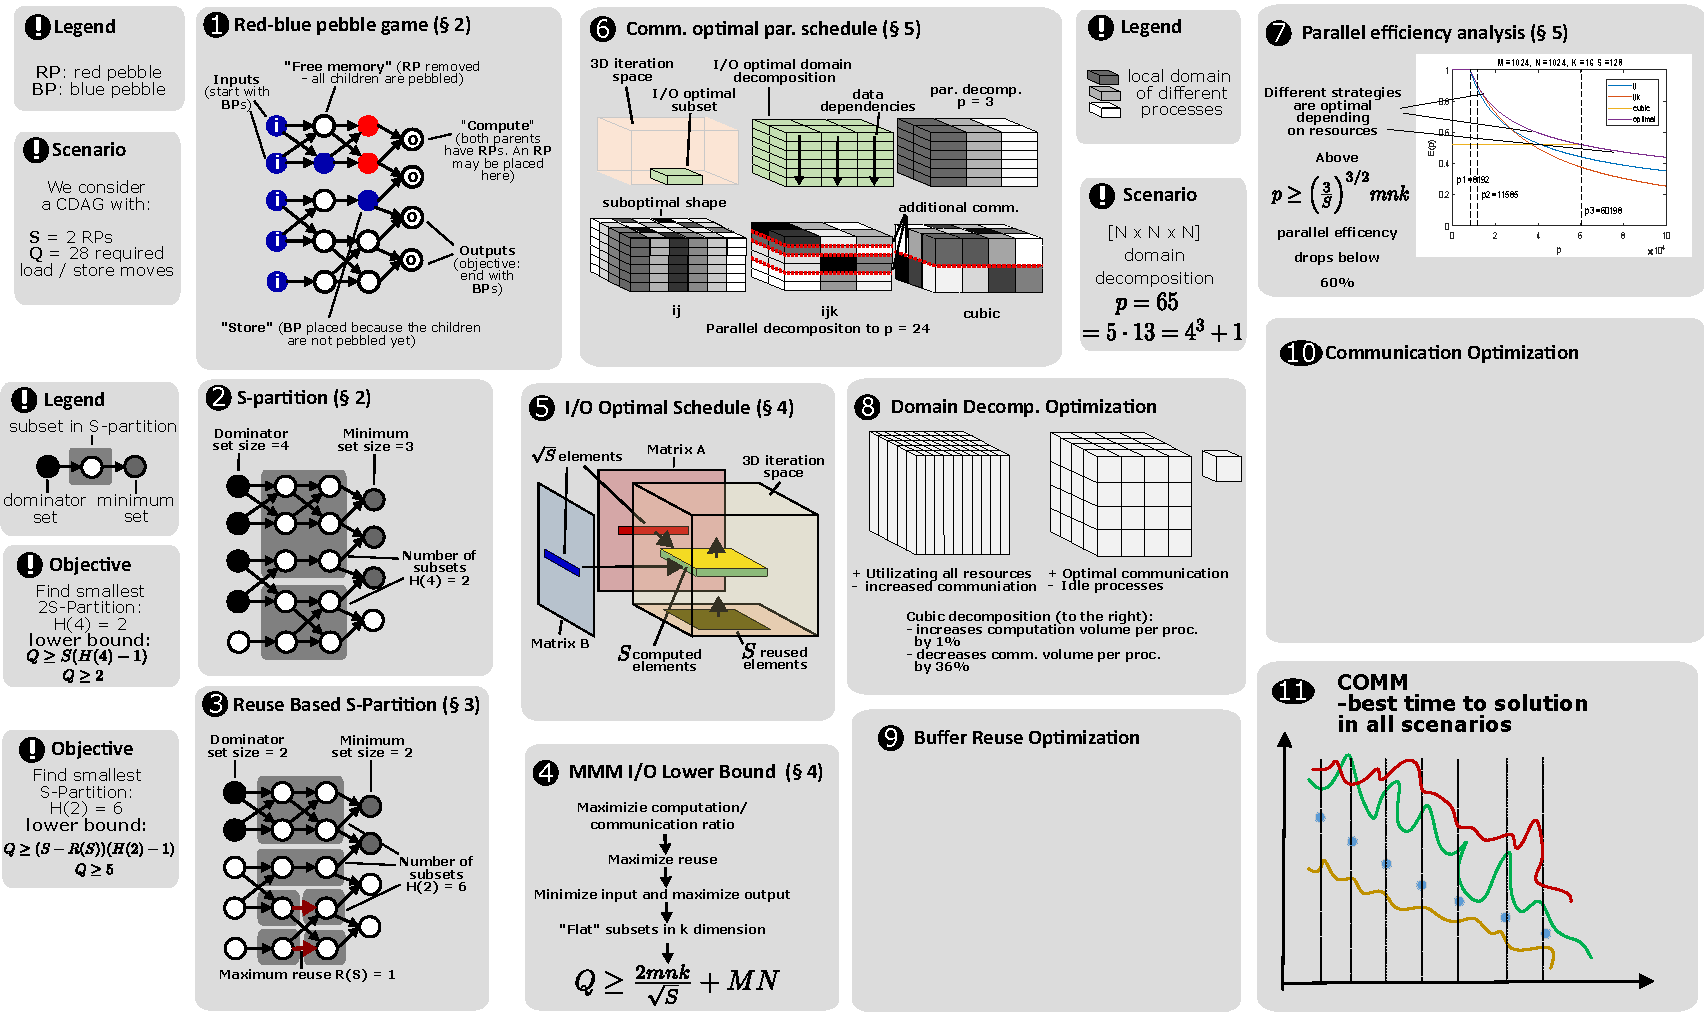
\includegraphics[width=\textwidth]{figures/paperOrganization}
%  \caption{Achieving data movement optimal MMM in eleven simple 
%    steps: (I) I/O lower bounds and red-blue pebble game, (II) 
%    $2S$-partition lemma, (III) reuse-based lemma, (IV) MMM I/O 
%    lower 
%    bound, (V) I/O optimal schedule, (VI) communication optimal 
%    parallel schedule, (VII) parallel efficiency analysis, (VIII) 
%    buffer optimization, (IX) communication optimization, (X) 
%    process 
%    decomposition optimization, (XI) best time-to-solution 
%    result. }
%  %
%  \label{fig:paperOrganization}
%\end{figure*}
% OLD long MMM par below
%
%     Matrix-matrix multiplication (MMM) is one of the most fundamental building
%     blocks in scientific computing. It is widely used not only in virtually 
%all
%     linear algebra algorithms (Cholesky and LU
%     decomposition~\cite{meyer2000matrix}, eigenvalue
%     factorization~\cite{chatelin2012eigenvalues}, triangular
%     solvers~\cite{linearAlgebraLAPACK}), but also in numerous graph 
%algorithms such
%     as Breadth-First Search (BFS)~\cite{cormen2009introduction} or Triangle
%     Counting~\cite{azad2015parallel} through efforts such as
%     GraphBLAS~\cite{kepner2016mathematical}. Other use cases include spectral
%     clustering~\cite{ng2002spectral} or machine
%     learning~\cite{abadi2016tensorflow}.  Thus, accelerating MMM routines is 
%of
%     great significance for many domains.

Matrix-matrix multiplication (MMM) is one of the most fundamental building
blocks in scientific computing, used in linear algebra algorithms (Cholesky and
LU decomposition~\cite{meyer2000matrix}, eigenvalue
factorization~\cite{chatelin2012eigenvalues}, triangular
solvers~\cite{linearAlgebraLAPACK}), machine
learning~\cite{abadi2016tensorflow}, graph
processing~\cite{cormen2009introduction, azad2015parallel,
kepner2016mathematical, ng2002spectral, slimsell, maciejBC}, or computational 
chemistry~\cite{joost}. Thus, accelerating MMM routines is 
of great significance for many domains. 
Minimizing the amount of transfered data is essential for high--performance 
and  power--efficient MMM.
%Due to the relative increase of 
%input-output (I/O) cost compared to computation, I/O-minimizing techniques are 
%essential to increase performance of those routines on modern architectures.
In this paper we use the term I/O both for data transfers across the memory 
hierarchy (\emph{vertical I/O}) and between processes in a distributed machine 
(\emph{horizontal I/O}).

Modern parallel machines with deep memory hierarchies offer high performance 
for highly regular computations, such as ``classical'' MMM algorithms which 
perform 
$n^3$ multiplications. Another class of algorithms
are Strassen-like routines~\cite{Strassen}, which asymptotically reduce the
number of multiplications. However, in practice they are often 
slower~\cite{strassenVsClassic}. Therefore, in this work, we focus only on a 
former class.
%
%\greg{revert. Start with architectures, Modern parallel machines with deep 
%memory hierarchies offer premises of high performance. Unfortunanately, 
%strassen are slow }
%In this work, we focus only on the ``classical'' MMM algorithms which perform 
%$n^3$ multiplications. 


\begin{table*}
	%	\vspace{-1em}
	%
%	\setlength{\tabcolsep}{4pt}
%	\renewcommand{\arraystretch}{1}
	\centering
	%\footnotesize
	\fontsize{0.26cm}{0.4cm}\selectfont
%	\scriptsize
	\sf
	\hskip-0.5em
	\begin{tabular}{lllll}
		%
		\multicolumn{5}{c}{$C=AB, A \in \mathbb{R}^{m \times k}$ and $ B \in 
			\mathbb{R}^{k \times n}$} \\
		%\vspace{-0.5em}
		%
		\toprule
		& \textbf{2D~\cite{summa}} & \textbf{2.5D~\cite{25d}} & 
		\textbf{recursive~\cite{CARMA}} & \textbf{COMM} \\
		%
		\midrule
		Input:
		%\textbf{Input}
		&
		User--specified grid
		&
		\makecell[l] {
			Available
			memory
		}
		&
		\makecell[l] {
			Available memory, 
			matrix dimensions}
		& 
		\makecell[l] {
			Available memory, 
			matrix dimensions}
		\\
		%
		%	\rowcolor{gray}
		\textbf{Step 1}
		%		\makecell[l]{\textbf{process} %\\
		%			\textbf{decomposition} \\
		%			$\left[p_m \times p_n \times p_k\right]$}
		&
		Split $m$ and $n$
		&
		Split $m$, $n$, $k$
		& 
		\makecell[l] {
			Split recursively the largest dimension
		}
		& 
		\makecell[l] {
			Find the optimal
			sequential schedule
		}
		\\
		%	\midrule
		\textbf{Step 2}
		&
		\makecell[l] {
			Map matrices 
			to process grid
		}
		&
		\makecell[l] {
			Map matrices 
			to process grid
		}
		&
		\makecell[l] {
			Map matrices 
			to recursion tree
		}
		& 
		\makecell[l] {
			Map sequential 
			domain to matrices
		}
		\\
		\midrule
	%	\textbf{Observations:}
		&
		\makecell[l] {
			\faThumbsDown Requires manual tuning  \\
			\faThumbsDown Asymptotically
			more comm.  
		}
		&
		\makecell[l] {
			\faThumbsOUp Optimal for $m=n$  \\
			\faThumbsDown Inefficient for 
			$m \ll n$ 
			or $n \ll m$  \\
			\faThumbsDown Inefficient for some $p$
		}
		&
		\makecell[l] {
			\faThumbsOUp Asymptotically 
			optimal 
			for all  $m,n,k,p$  \\
			\faThumbsDown Up to $\sqrt{3}$ more comm.\\
			\faThumbsDown $p$ must be 
			a power of 2  
		}
		& 
		\makecell[l] {
			\faThumbsOUp ~ ~Optimal for 
			all $m,n,k$  \\
			\faThumbsOUp ~ ~Optimal for
			all $p$  \\
			\faThumbsOUp \faThumbsOUp ~Highest performance
		}
		\\
		\bottomrule
		%
	\end{tabular}
	%
	\caption{Intuitive comparison between the COMM algorithm and the 
		state-of-the-art 2D, 2.5D, and recursive decompositions.
	}
	%
	\vspace{-0.5em}
	%
	\label{tab:intro}
\end{table*}


\begin{figure}
%	\vspace{-3em}
	\centering
	%
	\subfloat[square matrix]{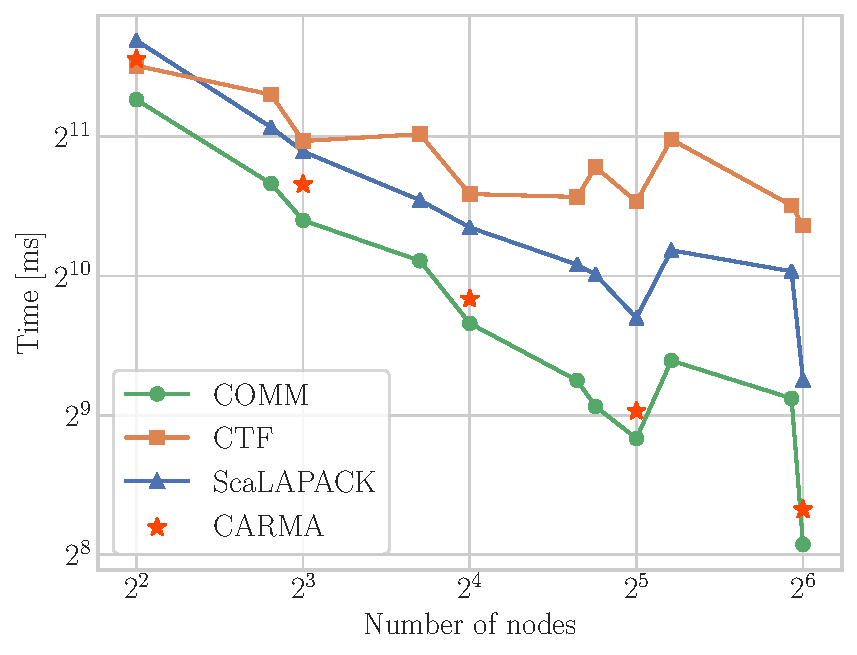
\includegraphics[width=0.23\textwidth]
		{results/square_strong_scaling}\label{fig:introPlot:f1}}
	%
	\hfill
	%
	\subfloat["skinny" matrix]{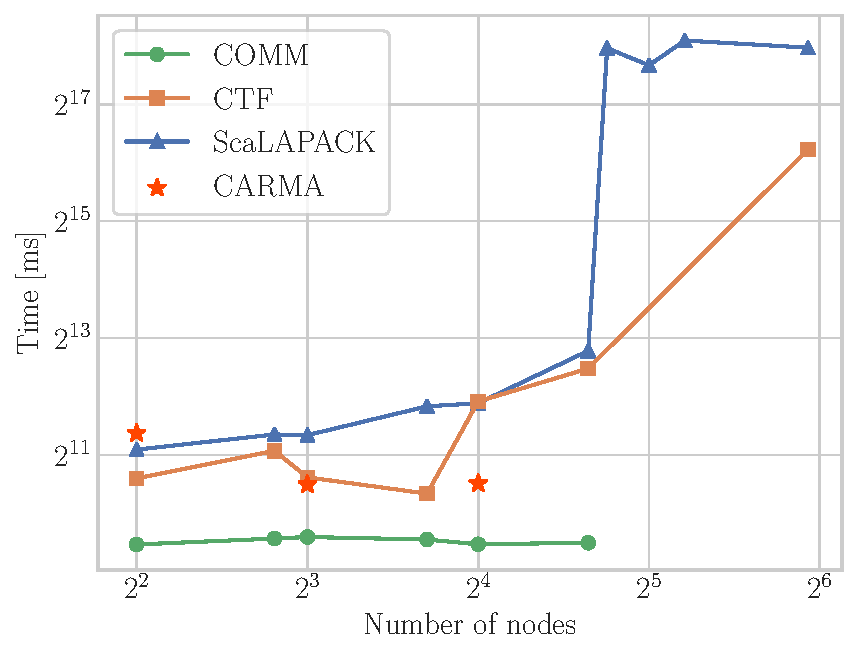
\includegraphics[width=0.23\textwidth]
		{results/thin_strong_scaling}\label{fig:introPlot:f2}}
	%
	\vspace{-0.5em}
	\caption{Total MMM runtime of ScaLAPACK~\cite{scalapack} (2D 
	decomposition), CTF~\cite{cyclops} (2.5D decomposition),  
	CARMA~\cite{CARMA} (recursive)  COMM (this paper) algorithms. 
	See~\cref{sec:evaluation} for our evaluation 
	methodology. }
	\label{fig:introPlot}
	\vspace{-1em}
\end{figure}

The analysis of I/O--minimizing MMM algorithms has been an active topic of 
research 
for a 
long time. 
A first I/O lower bound in a two-level 
memory
model, $\Omega\left({n^3}/{\sqrt{S}}\right)$, where $S$ is the size of the fast
memory\footnote{Throughout this paper we use the original notation from Hong
and Kung to denote the memory size $S$. In literature, it is also common to use
the symbol $M$~\cite{externalMem,IronyMMM, parallelExMem}.} and $n$ is the
number of rows of a square matrix, was proven nearly 40 years ago by
Hong and Kung~\cite{redblue}.
%
%	and denote the memory size $M$. Hong and Kung used the symbol $S$.}. 
%
Irony et al.~\cite{IronyMMM} extended this
result to a parallel machine with $p$ processes,
each having a fast private memory of size~$S$, proving the
$\frac{n^3}{2\sqrt{2}p\sqrt{S}} - S$ 
%$\Omega\left({n^3}/{p\sqrt{S}}\right)$ 
lower bound on the communication volume 
per 
process.
%
%Various optimizations 
%Ever since then, those bounds serve as a
%driving force in developing better algorithms. \mac{This sounds a bit weird -
%why are the bounds a driving force? You can also see them as, well, bounds? I
%would probably remove it} This evolution includes optimizations like
%parallelization~\cite{parallelMMM}, tiling~\cite{tiling}, 2D~\cite{summa} and
%3D~\cite{summa3d} domain decomposition or data layout
%optimization~\cite{scalapackLayout}.
%
If $S$ is bounded by the input size ($pS \in \Theta(n^2)$), the bound
$\Omega\left({n^2}/{\sqrt{p}}\right)$  is asymptotically attainable by
algorithms such as Cannon's~\cite{Cannon} or SUMMA~\cite{summa}. In the
presence of extra memory ($pS \in \Theta(p^{1/3} n^2)$), the 3D
decomposition~\cite{summa3d} yields a better asymptotic bound
$\Omega\left({n^2}/{p^{2/3}}\right)$. The 2.5D algorithm by Solomonik
and Demmel~\cite{25d} effectively interpolates
between those two results, depending on the available
memory.

Recent efforts focus on accelerating 
non-square matrices. Such matrices are common in many
relevant areas, for example in machine learning
\cite{rectangularML} or computational chemistry~\cite{rectangularChemistry}.
%
Yet, Demmel et al.~\cite{CARMA} showed
that algorithms optimized for squared matrices often perform poorly
when matrix dimensions vary significantly~\cite{CARMA}. They introduced CARMA, 
a recursive algorithm that achieves asymptotic lower bounds for all
configurations of dimensions and memory sizes.  

%\mac{You must mention CTF after
%this e-mail exchange with Edgar} \greg{I need results from Marko}

%
%\mac{This ``intra-node memory sizes'' comes out of the blue - why do we care?
%So far, you only motivated shapes. If this memory size parameter is crucial
%for later sections, I would also suggest a small paragraph for this, with
%concrete examples on why it matters}\greg{changed to just "memory" and there
%are referenced to this}

%
%\begin{table}
%	%	\vspace{-1em}
%	%
%	\setlength{\tabcolsep}{4pt}
%	\renewcommand{\arraystretch}{1}
%	\centering
%	%\footnotesize
%	\scriptsize
%	\sf
%	%
%	%		\begin{tabular}{llll}
%	%		%
%	%		\toprule
%	%		%\vspace{-0.5em}
%	%		%
%	%		& \textbf{Step 1} & \textbf{based on...} & \textbf{Step 2} \\
%	%		%
%	%		\midrule
%	%		%
%	%		\textbf{2D~\cite{summa}}
%	%		%		\makecell[l]{\textbf{process} %\\
%	%		%			\textbf{decomposition} \\
%	%		%			$\left[p_m \times p_n \times p_k\right]$}
%	%		&
%	%		split $m$ and $n$
%	%		&
%	%user provided grid
%	%		& 
%	%
%	%\makecell[l] {
%	%	map problem \\
%	%	to process grid
%	%}
%	%		\\
%	%		\textbf{2.5D~\cite{25d}}
%	%		&
%	%				split $m$, $n$, and $k$
%	%		&
%	%		available memory
%	%		&		
%	%		\makecell[l] {
%	%			map problem \\
%	%			to process grid
%	%		}
%	%		\\
%	%%		\midrule
%	%				\textbf{recursive~\cite{CARMA}}
%	%		&
%	%				\makecell[l] {
%	%			split recursively\\ largest dimension
%	%		}
%	%		&
%	%		\makecell[l] {
%	%			available memory, \\
%	%			matrix dimensions}
%	%		&
%	%		\makecell[l] {
%	%			map problem \\
%	%			to recursion tree
%	%		}
%	%	%
%	%	\\
%	%  \textbf{COMM (this paper)}
%	%	&
%	%		\makecell[l] {
%	%		find optimal\\
%	%		sequential schedule
%	%	}
%	%	&
%	%\makecell[l] {
%	%	available memory, \\
%	%	matrix dimensions}
%	%			& 
%	%	\makecell[l] {
%	%		map sequential \\
%	%		domain to problem
%	%	}
%	%		\\
%	%		\bottomrule
%	%		%
%	%	\end{tabular}
%	%
%	%
%	%
%	%
%	%	\hspace{-2em}
%	\hskip-3em
%	\begin{tabular}{lllll}
%		%
%		\multicolumn{5}{c}{$A \in \mathbb{R}^{m \times k}$ and $ B \in 
%			\mathbb{R}^{k \times n}$} \\
%		%\vspace{-0.5em}
%		%
%		& \textbf{2D~\cite{summa}} & \textbf{2.5D~\cite{25d}} & 
%		\textbf{recursive~\cite{CARMA}} & \textbf{COMM} \\
%		%
%		\midrule
%		%
%		%	\rowcolor{gray}
%		\textbf{Step 1}
%		%		\makecell[l]{\textbf{process} %\\
%		%			\textbf{decomposition} \\
%		%			$\left[p_m \times p_n \times p_k\right]$}
%		&
%		split $m$ and $n$
%		&
%		split $m$, $n$, $k$
%		& 
%		\makecell[l] {
%			split recursively\\ largest dimension
%		}
%		& 
%		\makecell[l] {
%			find optimal\\
%			sequential schedule
%		}
%		\\
%		\textbf{based on:}
%		&
%		user input
%		&
%		\makecell[l] {
%			available\\
%			memory
%		}
%		&
%		\makecell[l] {
%			available memory, \\
%			matrix dimensions}
%		& 
%		\makecell[l] {
%			available memory, \\
%			matrix dimensions}
%		\\
%		%	\midrule
%		\textbf{Step 2}
%		&
%		\makecell[l] {
%			map matrices \\
%			to process grid
%		}
%		&
%		\makecell[l] {
%			map matrices \\
%			to process grid
%		}
%		&
%		\makecell[l] {
%			map matrices \\
%			to recursion tree
%		}
%		& 
%		\makecell[l] {
%			map sequential \\
%			domain to matrices
%		}
%		\\
%		\midrule
%		\textbf{results in:}
%		&
%		\makecell[l] {
%			\faThumbsODown Requires user
%			\\ input  \\
%			\faThumbsODown Asymptotically \\
%			more comm.  
%		}
%		&
%		\makecell[l] {
%			\faThumbsOUp Optimal for $m=n$  \\
%			\faThumbsODown Bad for $m \ll n$ \\
%			or $n \ll m$  \\
%			\faThumbsODown Bad for some $p$
%		}
%		&
%		\makecell[l] {
%			\faThumbsOUp Asymptotically \\
%			optimal for all $m,n,k,p$  \\
%			\faThumbsODown Up to $\sqrt{3}$ more comm.\\
%			\faThumbsODown $p$ must be \\
%			a power of 2  
%		}
%		& 
%		\makecell[l] {
%			\faThumbsOUp Optimal for \\
%			all $m,n,k$  \\
%			\faThumbsOUp Optimal for \\
%			all $p$  
%		}
%		\\
%		\bottomrule
%		%
%	\end{tabular}
%	%
%	\caption{Intuitive comparison between the COMM algorithm and the 
%		state-of-the-art 2D, 2.5D, and recursive decompositions.
%	}
%	%
%	\vspace{-0.5em}
%	%
%	\label{tab:intro}
%\end{table}


Unfortunately, we observe several problems with state-of-the art
algorithms, including ScaLAPACK~\cite{scalapack} (an implementation of
SUMMA), Cyclops Tensor Framework (CTF)~\cite{cyclops} (an implementation of the 
2.5D MMM algorithm), or CARMA~\cite{CARMA}. ScaLAPACK supports
only the 2D~decomposition, which is communication--inefficient in a presence of 
extra memory. Also, it requires a 
user to
fine-tune parameters such as block sizes or a process
grid size. The available CARMA specification supports only scenarios when the 
number of
processes is a power of two, a serious limitation, as the number of processes 
is usually determined by the available
hardware resources.
%  For example, Piz Daint, the
%third fastest supercomputer in 2017, has 1,813 CPU nodes, which are
%impossible to arrange in a cubic grid. 
CTF can utilize any number of processes, but its decompositions may be far from 
optimal~(\cref{sec:results}). We also emphasize that 
\emph{asymptotic 
complexity is an insufficient measure of speedup}. For instance, the
Coppersmith--Winograd algorithm~\cite{coppersmith} achieves computational
complexity of $\mathcal{O}(n^{2.376})$, but its constant terms are 
prohibitively big and
make it slower in practice than the classical $\mathcal{O}(n^{3})$ algorithms. 
We later (\cref{sec:evaluation}) identify similar overheads in CARMA. Our 
observations are summarized in Table~\ref{tab:intro}. Their practical 
implications are shown in the Figure~\ref{fig:introPlot}, where we see that all 
the discussed algorithms perform poorly for some configurations. 




%%
%, a common case in practice
%\mac{Again, at least one sentence to this. Why not suitable? What happens?
%'Unsuitable - extremely confusing word...}. For example, Del Ben et
%al.~\cite{joost} used the "tall and skinny" matrices to simulate water
%molecules' interaction \mac{This sentence is completely out of the place. You
%just finished writing about why CARMA and others are bad. And suddenly an
%example of using tall and skinny matrices. Must go elsewhere}. Matrix dimension
%sizes are determined by their number - e.g., for 64 molecules, M=n=8704 and
%k=933888 \mac{Some comment as above - this must go elsewhere}. The number of
%processes, on the other hand, is often determined by available resources and is
%rarely a divisor of the problem size. 

In this work, we present COMM (Communication Optimal Matrix Multiplication): 
an algorithm that takes a new approach to multiplying
matrices and alleviates the above issues. COMM is I/O optimal \emph{with regard 
to all constant factors}
for \emph{all combinations of parameters}. The driving idea is to start with 
the optimal sequential schedule, which we then parallelize, deriving a process 
grid. This is in contrast with the other discussed algorithms, which fix the 
process grid upfront and then map it to a sequential schedule for each 
process.   We outline the
algorithm in~\cref{sec:commDescr}.
%
To prove its optimality,  we first provide a new 
constructive proof of a sequential I/O lower bound~(\cref{sec:seqScheduling}),  
then we
derive the communication cost of  
parallelizing the sequential
schedule~(\cref{sec:parStrategies}), and finally we construct an I/O optimal 
parallel 
schedule~(\cref{sec:parScheduling}). 
The detailed communication analysis of COMM, 2D, 3D, and 
recursive decompositions is
presented in Table~\ref{tab:summary}. Our algorithm reduces the data 
movement volume by a factor of up to $\sqrt{3} \approx 1.73$x compared to 
the 
asymptotically optimal recursive decomposition and up to 
$\max\{n,m,k\}$ times compared to the 2D
algorithms, like Cannon's~\cite{generalCannon} or SUMMA~\cite{summa}.


Unlike CARMA, which is based on recursive data layout, our implementation
enables transparent integration with the ScaLAPACK
format~\cite{scalapackLayout} and delivers near-optimal computation throughput.
%
We later (\cref{sec:implementation}) show that the obtained schedule 
naturally expresses
computation--communication overlap, 
%
%\mac{if it's true, I would also add here
%``unlike the existing approaches''}\greg{not sure about this part}
%
enabling even higher speedups
using Remote Direct Memory Access (RDMA).
%
%We further motivate our work in Figure~\ref{fig:motivation-page-1} that shows
%the advantages of our algorithm over the state of the art \greg{what do you 
%want to put here?}.
%%
% Other incorporated techniques include buffer and layout optimization to 
%further
% accelerate the execution time. 
%
Finally, our I/O optimal approach is
easily generalizable to other linear algebra kernels. 
%
We provide the following contributions:

\begin{itemize}[leftmargin=1em]
%
\item We propose COMM: a distributed MMM algorithm that is I/O optimal for 
\emph{any combination of parameters}. 
%
%the algorithm achieving up to ?? speedup (?? on average) in
%the total runtime of the MMM scheme over the existing state-of-the-art 
%implementations,
%
\item Based the red-blue pebble game 
abstraction~\cite{redblue}, we provide a new proof (constructive) of
the sequential MMM I/O lower bound.  The proof delivers tight
constant factors (\cref{sec:seqOpt}). We extend this proof to parallel machines 
(\cref{sec:parScheduling}).
%
%\item we \mac{We} confront the parallel efficiency of our schedule with 
%existing state-of-the art 2D and 3D matrix
%multiplication variants \mac{state what is the outcome of this confrontation,
%we must contribute sth!} (~\cref{sec:parOptimality} \mac{use cref}),
%
\item We reduce memory footprint for communication buffers and guarantee
minimal reshuffling of input data by using a block-cyclic data layout
(\cref{sec:datalayout}) and a static buffer pre-allocation
(\cref{sec:bufferReuse}), providing compatibility with the
ScaLAPACK format~(\cref{sec:implementation}).
% Our design provides better compatibility with the
%ScaLAPACK format than CARMA (\cref{sec:implementation}).
%
\item We utilize the computation--communication overlap, which enables
even higher speedups with RDMA (\cref{sec:implementation}),
%
\item We evaluate the performance of COMM, ScaLAPACK, CARMA and CTF on the CSCS 
Piz 
Daint supercomputer for an
extensive selection of problem dimensions, memory sizes, and numbers of
processes, showing the speedup of up to \greg{Missing} (\greg{Missing} on 
average) 
(~\cref{sec:results}).
%
\end{itemize}

%
%%
%\mac{Also, see the long comment on top-down above. These 3 reasons here are not
%enough to understand why this thing is called bottom-up.}.
%%
%Our schedule is based on the ``S--partitioning'' concept from the Hong and 
%Kung's 
%red--blue
%pebble game~\cite{redblue} to derive the best (i.e., optimal) partitioning
%routine that minimizes data movement for a given MM product in a parallel
%setting. The model is simplistic and it transparently applies both to 
%distributed and shared memory machines for all possible combinations of 
%parameters.
%%
%We illustrate an intuitive comparison of our bottom-up approach versus the
%classic top-down schemes in Figure~\ref{fig:topdown-vs-bottomup}.

%
%  - \mac{Using such dashes
%is a bad idea in papers, reads bad and informal. Colons are better} it 
%minimizes both the number of I/O 
%operations (vertical data movement across the memory hierarchy) and 
%communication between processes in distributed setting (horizontal data 
%movement) \mac{I thought at this point it's somewhat weird that you combine 
%these two
%and name them in this way. I
%mean, distributed *IS* actually I/O, right? Not disk I/O, but still I/O (NIC, 
%network).
%I would (1) think how to maybe name it a bit better, and (2) investigate
%thoroughly the connection and the overlapping papers}. Our key idea is to 
%``invert'' the traditional ``top-down''
%approach for multiplying matrices, shared by all the mentioned state-of-the-art
%algorithms, that fix the domain partitioning in some predefined fashion
%(2D~\cite{Cannon}, 2.5D~\cite{25d}, or
%recursive~\cite{CARMA}) \mac{The word ``invert'' and ``top-down'' is confusing.
%You just write it down like sth obvious, but it's not obvious (calling all 
%these
%schemes top-down is not obvious). I would suggest to maybe first provide 1-3 
%sentences
%that will straightforwardly explain on why all these schemes are called 
%``top-down'',
%focusing (in this explanation) ALSO on the downsides of this approach. Only 
%after, 
%I would state that we do bottom-up, and invert the top-down, but write it in 
%such
%a way that it is clear WHAT EXACTLY is inverted in the top-down approach}.
%

%
% \mac{Do *not* refer to this figure here. This figure is very very complex and
% long. If you want a simple top-down VS bottom-up figure, it MUST focus ONLY
% on top-down vs bottom-up. Not on everything in the paper...}


%
%The overview of the paper's organization is presented in 
%Figure~\ref{fig:paperOrganization}.
%\mac{I would provide at least 2-3 sentences here (if you want to make it a 
%separate
%paragraph), OR merge this one sentence in some other paragraph.}

\vspace{-1em}
\section{Background}

In this section, we first describe our parallel machine 
model~\cref{sec:machineModel}, that transparently applies to both shared and 
distributed memory machines. We then define our optimization 
goal~\cref{sec:optGoals} in this model: ~\emph{the I/O cost}. 
In~\cref{sec:state-of-the-artAlgs} we provide a brief description and 
assumptions of the other state-of-the-art algorithms. Finally, the computation 
model~\cref{sec:compModel} 
introduces necessary concepts for our theoretical results: proofs of the I/O 
optimality of our sequential and parallel schedules. The most important symbols 
are gathered 
in 
Table~\ref{tab:symbols}.


\begin{table}[h]
\vspace{-0.5em}
\setlength{\tabcolsep}{2pt}
\renewcommand{\arraystretch}{0.7}
%
	\centering
	%\footnotesize
	\scriptsize
	%\ssmall
	\sf
	\begin{tabular}{@{}l|ll@{}}
		\toprule
		\multirow{5}{*}{\begin{turn}{90}\textbf{MMM}\end{turn}}
		& $m, n, k$& Matrix dimensions \\
		& $A, B$& Input matrices $A \in \mathbb{R}^{m \times k}$ and $ B \in 
		\mathbb{R}^{k \times n}$ \\
		& $C = AB$& Output matrix $C \in \mathbb{R}^{m \times n}$ \\
		& $p,S$& The number of processes and the memory size per process \\
		\midrule
		\multirow{13}{*}{\begin{turn}{90}\textbf{I/O complexity}\end{turn}}
		& $G$&A directed acyclic graph $G=(V,E)$\\
		%& $n,m$&Numbers of vertices and edges in $G$; $|V| = n, |E| = m$.\\
		& $S$ & The number of red pebbles (size of the fast memory)\\
		& $V_i$ & An $i$-th subcomputation of an $S$-partition \\
		& $Dom(V_i), Min(V_i)$ & Dominator and minimum sets of subcomputation 
		$V_i$\\
		& $V_{R,i}$ & \makecell[l]{The \emph{reuse set}: a set of vertices 
		containing red pebbles\\(just before $V_i$ starts) and used by $V_i$} \\
		& $H(S)$ & The smallest cardinality of a valid $S$-partition \\
		& $R(S)$ & The maximum size of the reuse set \\
		& $Q$ & The I/O cost of a schedule (a number of I/O operations) \\
		& $\rho_i$ & The computational intensity of $V_i$\\
		& $\rho = \max_i\{\rho_i\}$ & The maximum computational intensity\\
		\midrule
		\multirow{10}{*}{\begin{turn}{90}
				%
				%\makecell[l]{\textbf{parallel} 
				%	\\ \textbf{scheduling}}
				%
				\textbf{Scheduling}
			\end{turn}} 
		& $\mathcal{V}$ & The 3D iteration space of MMM 
		(\cref{sec:iterationSpace})\\         
		& \textbf{i},\textbf{j},\textbf{k} & Orthonormal vectors spanning 
		$\mathcal{V}$\\
		& \textbf{uv} & The plane spanned by vectors \textbf{u} and \textbf{v}\\
		& $\phi_{uv}(V)$ & The projection of subspace $V$ onto plane 
		\textbf{uv}\\
		& $\mathcal{S} = \{V_i\}$ & The sequential schedule (an ordered set of 
		 $V_i$) \\ 
		& $\mathcal{P} = \{\mathcal{S}_j\}$ & The parallel schedule (a set of 
		sequential schedules $\mathcal{S}_j$) \\
		& $\mathcal{D}_j = \bigcup_{V_i \in \mathcal{S}_j}V_i $ & The local 
		domain 
		(a set of vertices 
		of the sequential schedule $\mathcal{S}_j$ \\
		& $a,b$ &  Sizes of a local domain: $|\mathcal{D}_j| = a^2b$\\
		
		%\multirow{1}{*}{\begin{turn}{90}\textbf{.}\end{turn}}
		%                    & $S$ & The number of .\\
		\bottomrule
	\end{tabular}
	%\vspace{-0.5em}
	%
	%\vspace{-0.5em}
	%
	\caption{The most important symbols used in the paper.}
\vspace{-1em}
%
	\label{tab:symbols}
\end{table}
\vspace{-0.5em}


\subsection{Machine Model}
\label{sec:machineModel}

We model a parallel machine with $p$
processes, each with local memory of size $S$ words.
A process can send and receive from any other process up to $S$ words at 
a time.
To perform any computation, all the operands must reside in a process' local 
memory.
We assume a fully connected network. Furthermore, we assume that 
a computation is performed in synchronous rounds: in each round, processes 
first 
communicate with each other, then conduct computations on their local data.
Shared memory, if present, is modeled by an additional $(p+1)$-st process with  
unlimited local storage, that does not perform any computation. A communication 
between it and the remaining $p$ processes correspond to loading and storing 
from shared memory. Then, $S$ corresponds to a fast, private memory of each 
$p$ (e.g., a processor's cache), and the unlimited memory of $(p+1)$-st process 
is the shared storage.

This model is a generalization of established distributed machine 
models~\cite{CARMA,25d}, as it is applicable to shared memory and sequential 
machines (with $p=1$ and shared memory present). It is also an extension of a 
concurrent-read concurrent-write (CRCW) PRAM machine~\cite{pram}, as it allows 
processes to communicate not only through the shared memory, but also between 
one another.

%\mac{No other model details? Cost of operations, what about synchronization, 
%etc?} \greg{do you think it should be merged with "optimization goals" ? or to 
%keep it separated as it is}
%
%In addition to the \emph{I/O cost} $Q$, that is, a 
%maximum number of
%words communicated by any process, and the \emph{latency cost} $C_L$, 
%which is a number of
%required data transfers. A schedule is I/O optimal, if $W = Q$.


\subsection{Optimization Goals}
\label{sec:optGoals}
%
Throughout this paper we focus on the \emph{input/output (I/O) cost} $Q$ and 
the \emph{I/O optimality} of an algorithm.
%
The 
I/O cost~$Q$ is a number of words transferred during the execution 
of a schedule. On a sequential or shared memory machine equipped 
with small-and-fast and slow-and-big memories, these transfers are load 
and store operations from and to the slow memory (also called the 
\emph{vertical 
	I/O}). For a distributed machine with a limited memory per node, 
the 
transfers are communication operations between the nodes (also called the
\emph{horizontal I/O}). A schedule is \emph{I/O optimal} if it minimizes the 
I/O cost among all schedules of a given CDAG. 
The 
\emph{I/O complexity} of a 
CDAG is a lower bound of the I/O cost of a valid schedule.
%
Besides the I/O cost, we also model a \emph{latency cost} $L$, which is the 
minimal number of rounds necessary to perform al I/O operations.

%\greg{Not sure should we add this.}
%The shared and distributed machines may be nested of combined to model, e.g., 
%a 
%distributed machine with a local memory hierarchy per node. We then have two 
%I/O costs, vertical $W_v$: a total number of elements loaded from/stored to 
%the 
%nodes' memories, and horizontal $W_h$: a total number of elements communicated 
%between the nodes. of A schedule in this 
%model may be horizontally \emph{and/or} vertically optimal, if it minimizes 
%the 
%communication and/or load and store operations among all schedules.


\subsection{State-of-the-Art MMM Algorithms}
\label{sec:state-of-the-artAlgs}

Here, we briefly describe strategies of the existing MMM algorithms.
Throughout the whole paper, we consider matrix multiplication $C = 
AB$, where $A \in \mathbb{R}^{m \times k}, B \in \mathbb{R}^{k \times n},  C 
\in \mathbb{R}^{m \times 
	n}$, where $m$, $n$, and $k$ are matrix dimensions. Furthermore, we assume 
that the size of each element of matrices is one word, and that $S < 
\min\{mn, mk, nk\}$, that is, none of the matrices can entirely 
fit into single process' fast memory. 

We compare our algorithm with the 2D, 2.5D, and recursive 
decompositions. We assume a square process grid $[\sqrt{p}, \sqrt{p}, 1]$ 
for the 2D variant, analogously 
to the Cannon's algorithm~\cite{Cannon}, and a cubic grid $[\sqrt{p/c}, 
\sqrt{p/c}, c]$ for the 2.5D 
variant~\cite{25d}, where $c$ is the amount of the ``extra'' memory $c = 
pS/(mk 
+ nk)$. For the recursive decomposition, we assume that in each recursion level 
we split the largest dimension $m,n,$ or $k$ in half, until the local domain 
per 
process fits into the memory.
	The detailed complexity analysis of these decompositions is 
presented in 
Table~\ref{tab:summary}.
We note that ScaLAPACK or CTF can handle non-square 
decompositions. However, for ScaLAPACK this must be manually specified by a 
user, while CTF may find a suboptimal process decomposition if a number of 
processes has few factors, as discussed in~\cref{sec:decompArbitrary}. 
Moreover, 
in~\cref{sec:results} we compare the 
performance of COMM with the currently-newest implementations of ScaLAPACK, 
CARMA,  
and CTF, and measure a significant speedup in \emph{all} scenarios. 

\subsection{Computation Model}
\label{sec:compModel}

We now briefly specify a model of a \emph{general} computation; we use this
model in both the sequential and parallel setting.
An algorithm is modeled with the \emph{computational directed acyclic graph} 
(CDAG)
$G=(V,E)$~\cite{completeRegisterProblems,pebblegameregister,
registerpebblecolor}. A vertex $v \in V$ represents one
elementary operation in the given computation. An edge $(u,v) \in E$
represents that an operation $v$ depends on $u$. We call a set of all
immediate predecessors (or successors) of a vertex its \emph{parents} (or
\emph{children}).  Two selected subsets $I, O \subset V$ are \emph{inputs} and
\emph{outputs}, that is, sets of vertices that have no parents (or no children,
respectively).

\macb{Red-Blue Pebble Game} Hong and Kung's red-blue pebble game~\cite{redblue} 
is an abstraction modeling
an execution of an algorithm in a two-level memory structure with a
small-and-fast as well as large-and-slow memory. A red (or a blue) pebble
placed on a vertex of a CDAG denotes that a result of a corresponding 
elementary computation is inside
a fast (or slow) memory. 
In the initial/terminal configuration, only inputs/outputs of the CDAG have
blue pebbles.
%
There can be at most $S$ red pebbles used at any given time. A complete 
CDAG computation is a
sequence of moves that lead from the initial to the terminal pebble
configuration.
%
The allowed moves are:  placing a red pebble on any
vertex with a blue pebble (load),  placing a blue pebble on any
vertex with a red pebble (store),  placing a red pebble on a vertex
whose parents have all red pebbles (compute), removing any pebble, 
red or blue, from any vertex (freeing memory).
%  \mac{This definition does *not* what what red blue pebble game *is*.}
%  \greg{how should it look like?}
%\end{defn}

An I/O optimal execution (schedule) of a CDAG corresponds to a sequence of 
moves (called 
\emph{pebbling} of a graph) which minimizes load and store moves.
%
%A \emph{sequential schedule} $\mathcal{S}$ is a dependency-preserving sequence 
%of elementary operations
%(an ordering of the vertices of the CDAG). One schedule corresponds to one 
%topological
%ordering of $G$. 
In the MMM context, it is an order in which all $n^3$
multiplications in MMM are performed. A \emph{parallel schedule} $\mathcal{P} = 
\{\mathcal{S}_j\}$ is a collection of sequential schedules, such that each 
process $j = 1, \dots, p$ executes domain $\mathcal{S}_j$.

\section{COMM: High-Level Description}
\label{sec:commDescr}
%/
%\mac{The title is bad, you want sth like ``Optimal Matrix Products with COMM''}
%
%\mac{Greg, remember classes in Polish on writing essays and other literary
%forms?  How do we start? Usually in general, with some intro. Start with sth
%like ``'''}

\begin{figure}[!tbp]
	\centering
	%
	\subfloat[3D domain
	decomposition]{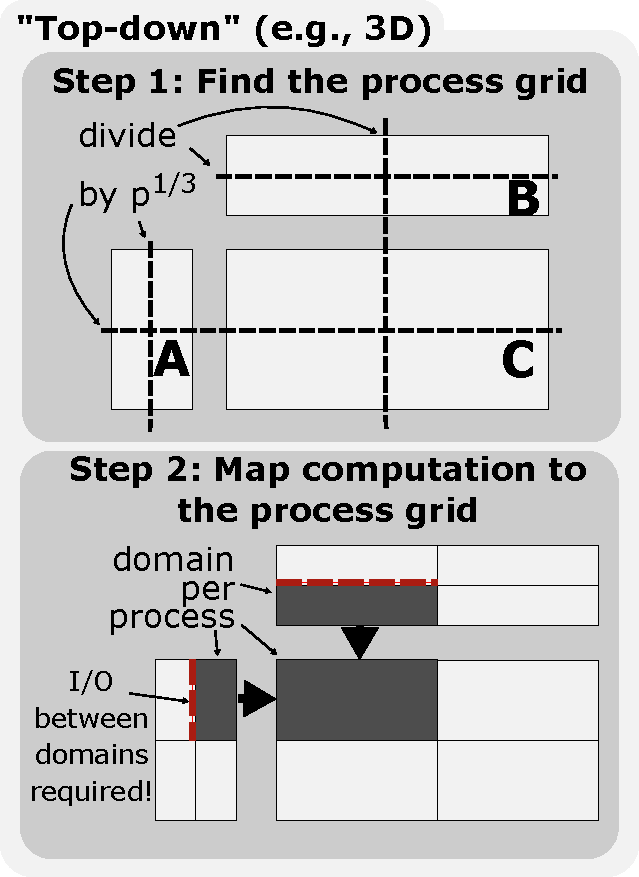
\includegraphics[width=0.23\textwidth]
		{figures/top-down-bottom-up-1}\label{fig:f1}}
	%
	\hfill
	%
	\subfloat[COMM decomposition]{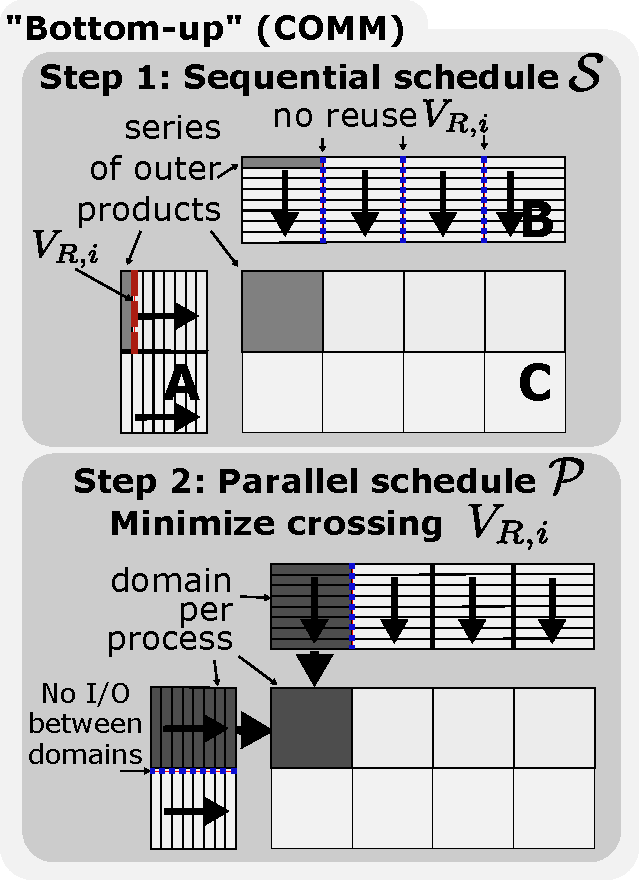
\includegraphics[width=0.23\textwidth]
		{figures/top-down-bottom-up-2}\label{fig:f2}}
	%
	\vspace{-1em}
	%
	\caption{Domain decomposition
		using $p=8$  processes. In the scenario (a), a straightforward 3D 
		decomposition
		divides every dimension in $p^{1/3}=2$. In the scenario (b), COMM 
		starts by
		finding an optimal sequential schedule and then parallelizes it 
		minimizing
		crossing data reuse $V_{R,i}$ (~\cref{sec:seqSched}). The total 
		communication volume is reduced by 17\%
		compared to the former strategy.}
	%
	\label{fig:topdown-vs-bottomup}
		\vspace{-1.5em}
\end{figure}

We now provide a high-level description of COMM, an algorithm that enables 
communication--optimal MMM.
COMM  decomposes processes by parallelizing the optimal sequential schedule
under given constraints: equal work distribution and memory size per process.
Such a local sequential schedule is independent of matrix dimensions.  Thus,
intuitively, instead of dividing  the global domain among $p$ processes (the
\emph{top-down} approach), we start from deriving an I/O optimal
\emph{sequential} schedule. We then parallelize it, minimizing the I/O and
latency costs $Q$, $L$ (the \emph{bottom-up} approach)
(Figure~\ref{fig:topdown-vs-bottomup}).
%This direction enables proving the optimality of the data movement, both
%horizontally and vertically (i.e., I/O) in our schedule, deriving all constant
%factors 
%(Figure~\ref{fig:topdown-vs-bottomup}).
Our experiments 
(\cref{sec:results}) confirm the theoretical analysis: COMM outperforms
all considered state-of-the-art algorithms.

The sketch of COMM is presented in Algorithm~\ref{alg:comm}.
In
Line~\ref{alg:line:findOptDomain} 
we derive an 
I/O--optimal sequential schedule for each process~(\cref{sec:parScheduling}). 
Each one of them is responsible for a subset 
of 
computation called a \emph{local domain} $\mathcal{D}$. $a_{opt}$ and 
$b_{opt}$ define the 
optimal size of $\mathcal{D}$, that is each $\mathcal{D}$ contains $a_{opt} 
\times a_{opt} 
\times b_{opt}$ vertices (multiplications to be performed).
%Lines~\ref{alg:line:aopt} and~\ref{alg:line:bopt}, we derive a 
%I/O--minimizing work distribution among $p$ 
%processes (\cref{sec:parScheduling}). Each process is responsible for a subset 
%of 
%computation called a \emph{local domain} $\mathcal{D}$ of. $a$ and $b$ are 
%optimal sizes of $\mathcal{D}$, such that $\mathcal{D}$ contains $a \times a 
%\times b$ vertices (multiplications to be performed).
 In 
Line~\ref{alg:line:fitranks}, we 
find a process
grid~$\mathcal{G}$ that evenly distributes this domain by the matrix dimensions 
$m,n$,
and $k$. If the dimensions are not divisible by $a_{opt}$ or $b_{opt}$, this
function also evaluates new values of $a$ and $b$ by fitting the best matching
decomposition, possibly discarding some processes~(\cref{sec:decompArbitrary}).
In Line~\ref{alg:line:datadecomp}, 
we decompose matrices $A, B$, and $C$ to the submatrices $A_l, B_l, C_l$ that 
are 
local for 
each process.
This decomposition is either  
%
%the local distribution of
%matrices $A_l$, $B_l$ and $C_l$ \mac{What are these matrices about?  Why use
%them? In the high-level description, this should be provided...} 
determined by a fixed input data layout, or redistributed using an optimal 
block-recursive
one~(\cref{sec:datalayout}). 
%Also, we compute a structure $Map$, which holds 
%the information about the decomposition of $A,B$ and $C$ to the local subsets.
%translates global matrix indices to a current owning process and a local offset
%in its memory.  
In Line~\ref{alg:line:stepsize} we compute a size of a 
communication step, that is, how many subcomputations 
(\cref{sec:seqSched}) are computed in a single round.
% Therefore, a size of a 
%local view $A_l$ 
%and $B_l$ is $a \times s$ (a size local view of $C_l$ is $a \times a$).
In Line~\ref{alg:line:steps} we 
compute the number of
sequential steps (Lines~\ref{alg:line:innerloopStart}
to~\ref{alg:line:innerLoopEnd}) in which every process: (1) distributes its
local data $A_l$ and $B_l$  among the grid $\mathcal{G}$ 
(Line~\ref{alg:line:distrData}),
% based on the $Map$ structure, 
and (2) multiplies locally $A_l$ and $B_l$
(Line~\ref{alg:line:compute}). Finally, the local partial results $C_l$ are
reduced over the grid $\mathcal{G}$ (line~\ref{alg:line:reduce}).

%\macb{I/O Complexity of COMM}
%We now analyze the complexity of COMM. 
%Lines~\ref{alg:line:findOptDomain}--\ref{alg:line:steps} require no 
%communication 
%(assuming that problem 
%parameters $m, n, k, p, S$ are already distributed at the start of the 
%program).
%The loop in Lines~\ref{alg:line:innerloopStart}--\ref{alg:line:innerLoopEnd} 
%executes $2ab/(S-a^2) = 
%\left\lceil{\min\{b, 2a^2/(S-a^2) \}} \right \rceil$ times. In 
%Line~\ref{alg:line:distrData}, each process receives $|A_l| + |B_l| = 
%\linebreak
%\left\lceil{\min\{2a, (S-a^2)/(2a) \}} \right \rceil$ elements, yielding in 
%total \linebreak$\left\lceil{\min\{2mnk/(p\sqrt{S + 1} - 1), 2(mnk/p)^{2/3} 
%\}} 
%\right 
%\rceil$ elements received throughout the loop. Sending the partial results in 
%Line~\ref{alg:line:reduce} adds $a^2 = \left\lceil{\min\{\sqrt{S+1} - 1, 
%(mnk/p)^{2/3}\}}\right\rceil$ communicated elements.
\macb{I/O Complexity of COMM}
We now analyze the complexity of COMM. 
Lines~\ref{alg:line:findOptDomain}--\ref{alg:line:steps} require no 
communication 
(assuming that problem 
parameters $m, n, k, p, S$ are already distributed at the start of the program).
The loop in Lines~\ref{alg:line:innerloopStart}-\ref{alg:line:innerLoopEnd} 
executes $\left\lceil{2ab/(S-a^2)}\right \rceil$ times. In 
Line~\ref{alg:line:distrData}, each process receives $|A_l| + |B_l|$ elements.
Sending the partial results in 
Line~\ref{alg:line:reduce} adds $a^2$ communicated elements. 
In~\cref{sec:parScheduling} we derive the optimal values $a_{opt} = 
\left\lceil{\min\{\sqrt{S}, 
(mnk/p)^{2/3}\}}\right\rceil$ and  $b_{opt} = 
\left\lceil{\max\{\frac{mnk}{pS}, 
(mnk/p)^{2/3}\}}\right\rceil$, which yields a total of 
$\min \Big\{S + 2 \cdot \frac{mnk}{p\sqrt{S}}, 3 
\left(\frac{mnk}{P}\right)^{2/3} \Big\}$ elements communicated.
%
% \linebreak$\left\lceil{\min\{2mnk/(p\sqrt{S + 1} - 1), 2(mnk/p)^{2/3} \}} 
%\right 
%\rceil$ elements received throughout the loop. 
%
%
%$|A_l| + |B_l| = \linebreak
%\left\lceil{\min\{2a, (S-a^2)/(2a) \}} \right \rceil$
%
%
%$a^2 = \left\lceil{\min\{\sqrt{S+1} - 1, 
%	(mnk/p)^{2/3}\}}\right\rceil$
%\begin{figure}
\begin{algorithm}
	\small
\caption{COMM} \label{alg:comm}
\begin{algorithmic}[1]
\Require $\text{matrices } A \in \mathbb{R}^{m \times k}, B \in 
\mathbb{R}^{k \times n}$,
\Statex {number of processes:  $p$, memory size: $S$}
\Ensure $\text{matrix } C = AB \in \mathbb{R}^{m \times n}$
%
%\State $a \gets \left \lfloor \min\Big\{\sqrt{S + 1} - 1, 
%\Big(\frac{mnk}{p}\Big)^{1/3} \Big\} \right \rfloor$ 
%\Comment{ (Equation \ref{eq:optTileShape})} 
%\label{alg:line:aopt}
%\State $b \gets \left \lfloor \max\Big\{\frac{mnk}{p(\sqrt{S + 1} - 1)^2}, 
%\Big(\frac{mnk}{p}\Big)^{1/3} \Big\} \right \rfloor$ 
%\label{alg:line:bopt}
%
\State $(a_{opt}, b_{opt}) \gets FindOptimalDomain(S,m,n,k,p)$ 
%\Comment{ Parallelize optimal sequential schedule} 
\label{alg:line:findOptDomain}
%
\State $(\mathcal{G}, a, b) \gets FitRanks(m,n,k,a_{opt},b_{opt},p)$ 
\label{alg:line:fitranks}
\ForAll{$p_i \in \left\{1 \dots p \right\}$} \textbf{in parallel}
\label{alg:line:outerloopStart}
%
%\State $\mathcal{D} \gets GetLocalDom(Grid,p_i)$ 
%\Comment{get local domain}
%\label{alg:line:localDomain}
\State $(A_l, B_l, C_l) \gets GetDataDecomp(A,B, \mathcal{G}, p_i)$ 
\label{alg:line:datadecomp}
\State $s \gets \left \lfloor{\frac{S - a^2}{2a}}\right \rfloor$
\Comment{size of a step}
\label{alg:line:stepsize}
\State $t \gets \left \lceil{\frac{b}{s}}\right \rceil$ 
\Comment{number of steps}
\label{alg:line:steps}
\For{$j \in \{1 \dots t\}$} 
\label{alg:line:innerloopStart}
\State $(A_l, B_l) \gets DistrData(A_l,B_l,\mathcal{G}, j, p_i)$ 
%\Comment{distr. inputs A and B}
\label{alg:line:distrData}
\State $C_l \gets Multiply(A_l, B_l,j)$ 
\Comment{compute locally}
\label{alg:line:compute}
\EndFor
\label{alg:line:innerLoopEnd}
\State $C_l \gets Reduce(C_l,D)$ \Comment{Reduce the partial results}
\label{alg:line:reduce}
\EndFor
\label{alg:line:outerLoopEnd}
\end{algorithmic}
\end{algorithm}
%\caption{COMM algorithm}
%\label{alg:COMM}
%\end{figure}


\section{Optimal Sequential MMM}
\label{sec:seqScheduling}

We now summarize our most important results related to the sequential I/O
optimality, both in a general context and for MMM. The detailed analysis, 
together with a proof of
Lemma~\ref{lma:reuse} and Theorem~\ref{thm:seqlowbounds}, may be found in the
attached supplementary material.

\subsection{I/O Lower Bounds for Arbitrary CDAGs}
\label{sec:iolowerbounds}

We first need to introduce the $S$-partition abstraction~\cite{redblue}, as we 
build our analysis on top of it.

\macb{$S$-Partitions}
%
Given a subset $V_i \in V$, define a \emph{dominator set} $Dom(V_i)$ as a set 
of 
vertices in $V_i$, such that every path from any input of a 
CDAG to any vertex in $V_i$ must contain at least one vertex in $Dom(V_i)$. 
Define 
also a \emph{minimum set} $Min(V_i)$ as a set of all vertices in $V_i$ which do 
not 
have any children in $V_i$.

Given a CDAG $G = (V,E)$, let $V_1, V_2, \dots V_h \in V$ be a series of 
subsets (called \emph{subcomputations}), such that: they are 
pairwise disjoint ($\forall_{i,j, i \ne j}V_i \cap V_j = \emptyset )$, they 
cover the whole CDAG ($\bigcup_i V_i = V$),
there are no cyclic dependencies between them ($\forall_{(u_1,v_1) \in E}: (u_1 
\in V_i \land v_1 \in V_j  \land i \ne j) \implies \nexists_{(u_2,v_2) \in E}: 
u_2 \in V_j \land v_2 \in V_i$), and their dominator and minimum sets are 
smaller than $S$ ($\forall_i (|Dom(V_i)| \le S \land |Min(V_i)| \le S)$).
These subcomputations $V_i$ correspond to some execution order (a schedule) of 
a CDAG, such that at step $i$, only vertices in $V_i$ are pebbled. We call this 
series an \emph{$S$-partition} or a 
\emph{schedule} of a 
CDAG $\mathcal{S}(S) = \{V_1, \dots, V_h\}$.

We are now ready to present our key lemma that is later used to prove tight I/O 
lower 
bounds for 
MMM
(Theorem~\ref{thm:seqlowbounds}). 

\macb{General I/O Lower Bounds Lemma}
%
When a subcomputation $V_i$ ($i > 1$) begins, observe that some vertices may
already 
have red pebbles on them placed during some ``previous'' $V_j$ ($j < i$). 
Some 
of them may have children that are in $V_i$. Denote this set 
$V_{R,i}$. By 
definition, those vertices are inside the dominator set $V_{R,i} \subset 
Dom(V_i)$. We call 
these vertices a \emph{reuse set}, as they correspond to results from 
previous subcomputations that are reused by a subsequent computation without 
being stored and loaded from the slow memory. Denote the size of the largest 
reuse 
set as $R(S) = max_i|V_{R,i}|$. 
%Then, we have:

\begin{lma}
	\label{lma:reuse}
	%
	Denote $H(S)$ as the minimum number of subcomputations in any valid 
	$S$-partition of a CDAG $\ G=(V,E)$. Then,
	the minimal number $Q$ of I/O operations for any valid execution of $G$ 
	 is bounded by  
	
	\vspace{-1em}
	\begin{equation}
	%
	Q \ge (S - R(S)) \cdot (H(S) - 1)
	%
	\label{eq:reusebound} \end{equation}
	\vspace{-1em}
	
	\noindent
	Moreover: 
	
	\vspace{-1.5em}
	\begin{equation}\label{eq:reusebound-pmax}
	H(S) \ge \frac{|V|}{|V_{max}|}
	\end{equation}
	\vspace{-0.5em}
	
	\noindent
	where $V_{max} = \argmax_{V_i \in \mathcal{S}(S)}|V_i|$ is 
	the largest
	subset of vertices in $\mathcal{S}(S)$.
\end{lma}
 
From this lemma, we derive a following corollary that we use to prove a tight 
I/O lower bound for MMM (Theorem~\ref{thm:seqlowbounds}):

\begin{corollary*}[Computational intensity]
	\label{cor:q}
	Define the number of computations performed by $V_i$ for one loaded 
	element as the \emph{computational 
		intensity} $\rho_i = \frac{|V_i|}{S - V_{R,i}}$ of a subcomputation 
		$V_i$.
	Denote $\rho = \max_i(\rho_i) \le \Big(\frac{|V_{max}|}{S-R(S)}\Big)$ to be 
	the \emph{maximal computational intensity}.
	Then, the number of I/O operations $Q$ is bounded by:
	\begin{equation}
	Q \ge {|V|}/{\rho}
	\end{equation} 
\end{corollary*}

\subsection{Tight MMM I/O Lower Bound} 
\label{sec:seqOpt}
We first present our theorem of a tight sequential
MMM I/O lower bound. It provides an additive improvement over the bound $Q \ge 
\frac{2mnk}{S} - 2S$ by Smith and van de 
Gein~\cite{tightMMM}. Furthermore, the proof is constructive: it provides a 
corresponding schedule. In the proof ($\S$\textbf{B} included in the 
supplementary material), the \emph{largest reuse set size} $R(S)$ plays a 
fundamental 
role, as it precisely measures the number of elements that can be kept in a 
fast memory between the elementary subcomputations $V_i$.

\begin{thm}[Sequential MMM I/O lower bound] 
	%Multiplying matrices of sizes $m \times k$ and $k \times m $ in the 
	%computation 
	%model from Definition~\ref{df:redbluegame} requires a minimum number of 
	%I/O 
	%operations is $\frac{mnk}{\sqrt{S}} + mn$.
	Given a MMM CDAG of matrices of sizes $m \times k$ and $k \times m$,
	the minimum number of load and store operations in the red-blue pebble game 
	using $S$ red pebbles is $\frac{mnk}{\sqrt{S}} + mn$.
	\label{thm:seqlowbounds}
\end{thm}

This bound is achieved when the reuse set size is maximized $R(S) = (\sqrt{S + 
1} -1)^2$. This, in turn, requires that each subcomputation $V_i$ is formed by 
multiplying $\sqrt{S+1} -1$ elements of 
$A$ 
by $\sqrt{S+1} -1$ elements of $B$, resulting in $ (\sqrt{S + 1} -1)^2$ partial 
results of $C$, which form a reuse set $V_{R,i+1}$ for the next computation 
$V_{i+1}$.
 We then derive the maximum computational intensity 
$\rho = V_i/(S - R(S)) = 1 + S/2(\sqrt{S+1} - 1)$.
Throughout the paper, to simplify the formulas, we approximate $\sqrt{S + 1} -1 
\approx \sqrt{S}$.

\subsection{Optimal Sequential MMM Schedule} 
\label{sec:seqSched}
To generate a schedule based on the result from~\cref{sec:seqOpt}, we must 
express the MMM algorithm in a CDAG form. In a most straightforward 
implementation, the
cells of matrix $C$ are updated $k$ times. 
To remove the self loops corresponding to updating the values
of $C$, we express it in a Single Static Assignment (SSA) form~\cite{ssa}. This 
representation requires that each variable is assigned exactly once, forcing 
the updated values of $C$ to have $k$ \emph{versions}. Then, each of the $mnk$
updates of $C$ corresponds to a different vertex in a CDAG. We 
represent $C$ as a 3D array to keep track of all $mnk$ partial results, where 
the value of $C(x,y,z)$ is equal to the first $z$ updates of cell $(x,y)$.  
Then, the I/O optimal sequential schedule is presented in 
Listing~\ref{lst:pseudocode}:

%\mac{What is $V(x,y,z)$?}\greg{is it getting better?}

\begin{lstlisting}[float=h, caption={Pseudocode of the I/O optimal sequential 
MMM in
the Single 
Static Assignment (SSA) form.},label=lst:pseudocode]
for ($i_1 = 1;\quad i_1 \le m/\sqrt{S};\quad ++i_1$) 
	for ($j_1 = 1;\quad j_1 \le n/\sqrt{S};\quad ++j_1$)
		for ($r = 1;\quad r \le k;\quad ++r$) 
			// An elementary subcomputation $V_i$
			for ($i_2 = i_1 \cdot \sqrt{S};\quad i_2 < (i_1+1) \cdot  
			\sqrt{S};\quad ++i_2$)
				for ($j_2 = j_1 \cdot \sqrt{S};\quad j_2 < (j_1+1) \cdot 
\sqrt{S};\quad ++j_2$)
					$C(i_2,j_2,r) = C(i_2,j_2,r-1) + A(i_2,r) \cdot B(r,j_2)$
\end{lstlisting}
\noindent
We define that for all $i_1,i_2$, we have $C(i_2,j_2,0) = 0$, and that the 
$k$-th level 
of $C$ holds the final result:  $C(i_2, j_2, k) = AB(i_2,j_2)$.


%\macb{Discussion:} 
Theorem~\ref{thm:seqlowbounds} proves the (vertical) I/O 
optimality of 
the schedule presented in Listing~\ref{lst:pseudocode}. 
In~\cref{sec:parOptimality} we parallelize it with the minimal (horizontal) I/O 
cost, proving the optimality of COMM.
%
% and the
%optimal schedule (), where each each subcomputation 
%$V_i$ is formed :
%
%\begin{lstlisting}[float=h, caption=Pseudocode of the I/O optimal sequential 
%MMM, 
%label=lst:pseudocode]
%for ($i_1 = 1;\quad i _1 < m/\sqrt{S};\quad ++i_1$) 
%	for ($j_1 = 1;\quad n/\sqrt{S};\quad ++j_1$)
%		for ($r = 1;\quad r < k;\quad ++r$) 
%			// An elementary subcomputation $V_i$
%			for ($i_2 = i_1 \cdot \sqrt{S};\quad i_2 < (i_1+1) \cdot 
%			\sqrt{S};\quad ++i_2$)
%				for ($j_2 = j_1 \cdot \sqrt{S};\quad j_2 < (j_1+1) \cdot 
%				\sqrt{S};\quad ++j_2$)
%					$C(i_2,j_2) = C(i_2,j_2) + A(i_2,r) \cdot B(r,j_2)$
%\end{lstlisting}
%
%\mac{I would again provide a paragraph \macb{Discussion} that
%discusses insights in this subsection and from this theorem}
%\greg{i don't get it}

\section{Optimal Parallel Matrix Multiplication}
\label{sec:parOptimality}

We now derive a communication optimal parallel schedule from the results
derived in~\cref{sec:seqScheduling}. The key notion is the data reuse, that
determines not only the sequential execution, as discussed
in~\cref{sec:seqScheduling}, but also the parallel 
scheduling: if the data reuse spans across multiple local domains, then it has 
to be communicated, increasing the I/O cost 
(Figure~\ref{fig:topdown-vs-bottomup}).

\subsection{Iteration Space of MMM}
\label{sec:iterationSpace}
%
%In a most straightforward implementation of a classical MMM algorithm, the
%cells of matrix $C$ are updated $k$ times. To represent this algorithm as a
%CDAG, we express it in a Single Static Assignment (SSA) form~\cite{ssa} to 
%remove the self loops corresponding to updating the values
%of $C$. We use a 3D array $V$ to keep track of all $mnk$ partial results, 
%where 
%the value of $V(x,y,z)$ is equal to the first $z$ updates of cell $C(x,y)$.  
%Then, the algorithm may be written as a triple-nested loop:
%\mac{What is $V(x,y,z)$?}\greg{is it getting better?}
%
%\begin{lstlisting}[float=h!, caption={The pseudocode of a classical MMM using 
%the Single 
%Static Assignment (SSA) form.},label={lst:label}]
%for ($i_1 = 1;\quad i_1 < n;\quad ++i_1$)
%	for ($i_2 = 1;\quad j_2 < m;\quad ++i_2$) {
%		for ($i_3 = 1;\quad i_3 < k;\quad ++i_3$)
%			$V(i_1,i_2,i_3) = V(i_1,i_2,i_3 - 1) + A(i_1,i_3) \cdot B(i_3,i_2)$
%		$C(i_1,i_2) = V(i_1,i_2,k)$
%  }
%\end{lstlisting}

\begin{figure}
	\centering
	%
	\subfloat[MMM CDAG]{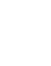
\includegraphics[width=0.168\textwidth]
		{figures/iterationSpace}\label{fig:f21}}
	%
	\hfill
	%
	\subfloat[cubic 
	decomposition]{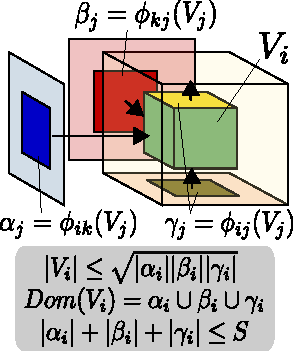
\includegraphics[width=0.15\textwidth]
		{figures/mmm_reuse_1}\label{fig:f22}}
	%
	\hfill
	%
	\subfloat["flat" 
	decomposition]{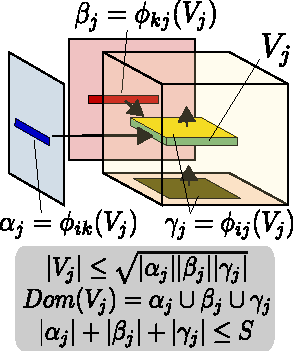
\includegraphics[width=0.15\textwidth]
		{figures/mmm_reuse_2}\label{fig:f23}}
	%
	% 
	%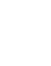
\includegraphics[width=0.26\textwidth]{figures/iterationSpace}
	\vspace{-1em}
		\caption{
			Case~\ref{fig:f21}:
		The MMM CDAG forming a 3D 
		iteration 
		space $\mathcal{V} \subset \mathbb{Z}^3$.
		Each 
		vertex 
		in $\mathcal{V}$
		(except of the vertices in the bottom layer) has 
		three parents - blue, 
		red, 
		and yellow, and one yellow child (except of vertices 
		in the top layer). 
		Case~\ref{fig:f22}: 
		Subcomputation $V_i$ with a maximum volume to surface ratio. Note that 
		in 
		a subsequent computation only one of the three planes 
		($\alpha_i$, $\beta_i$, or $\gamma_i$) 
		can 
		be reused. 
		Case~\ref{fig:f23}: Subcomputation $V_j$ with maximum computational 
		intensity $\rho_j$. Even though 
		$|V_i| > |V_j|$, we have
		$\rho_i = |V_i|/(|\alpha_i| + |\beta_i|) < \rho_j$.
	}
	\vspace{-1em}
%	\caption{
%		 An MMM CDAG forming a 3D 
%		iteration 
%		space $\mathcal{V} \subset \mathbb{Z}^3$. An input 
%		matrix A (blue 
%		vertices) 
%		is represented as 
%		its projection $\alpha = \phi_{ik}(\mathcal{V})$
%		on 
%		an \textbf{ik} plane - similarly, an input matrix B 
%		(red vertices) is a 
%		projection $\beta = \phi_{kj}(\mathcal{V})$ on the 
%		\textbf{kj} plane 
%		and an 
%		output 
%		matrix C (light yellow) 
%		is a 
%		projection $\gamma = \phi_{ij}(\mathcal{V})$ on the 
%		\textbf{ij} plane. 
%		Each 
%		vertex 
%		in this iteration space 
%		(except of the vertices in the bottom layer) has 
%		three parents - blue, 
%		red, 
%		and yellow and one yellow child (except of vertices 
%		in the top layer). 
%		$\alpha \cup \beta \cup \gamma$ form the dominator 
%		set $Dom(V_i)$.  
%		subcomputation $V_i \subset \mathcal{V}$ of an 
%		$S$-partition must 
%		satisfy 
%		$|Dom(V_i)| = |\alpha| + |\beta| + |\gamma| \le S$ 
%		(number of inputs 
%		must 
%		be 
%		smaller than $S$. \ref{fig:f22} 
%		optimal surface to volume subset shape. Note that in 
%		a subsequent 
%		subset computation only one of the three planes 
%		(blue, red or yellow) 
%		can 
%		be reused. \ref{fig:f23} the optimal subset shapes 
%		when 
%		data reuse is considered. Observe that even though 
%		$|V_i| > |V_j|$, but 
%		$|V_i|/(|\alpha_i| + |\beta_i|) < |V_j|/(|\alpha_j| + 
%		|\beta_j|)$.
%	}
	\label{fig:iterationSpace}
\end{figure}
%
%assuming that $C(i_1,i_2,0) = 0$ for all $i_1,i_2$. 

 Due to the
structure of the MMM algorithm (Listing~\ref{lst:pseudocode}), the 
corresponding 
CDAG can be represented as a 3D \emph{iteration
space} $\mathcal{V}$~\cite{tiling} (see Figure~\ref{fig:iterationSpace}). Let 
\textbf{i}, \textbf{j}, \textbf{k} be the orthonormal vectors spanning 
$\mathcal{V}$,
corresponding to the loops in Lines 1-3.  Denote a plane \textbf{uv} as a
plane spanned by vectors \textbf{u} and \textbf{v}, for some \textbf{u,v} $\in
\{\mathbf{i,j,k}\}$. Assume that $p = (i_1,i_2,i_3) \in \mathcal{V}$ is a point
in the iteration space. Then $\phi_{ij}(p) = (i_1,i_2)$ is a projection of this
point to the plane \textbf{ij}.

For each evaluation of Line 7, we map the elements \linebreak $C(i_2,j_2,r)$, 
$C(i_2,j_2,r-1)$, $A(i_2,r)$, and $B(r,j_2)$ to points in the iteration space 
$\mathcal{V}$. Elements from matrix $A$ lay on a plane \textbf{ik}. Similarly, 
elements from $B$ lay on a plane \textbf{kj} and the initial and final elements 
of $C$ lay on a plane \textbf{ij}. More formally, we map
$C(i_2,j_2,r)$ to a point
$v = (i_2,j_2,r) \in \mathcal{V}$, the element $C(i_2,j_2,r-1)$ to a point 
$\phi_{ij}(v) =
(i_2,j_2)$, $A(i_2,r)$ to a point $\phi_{ik}(v) = (i_2,r)$, and $B(r,j_2)$
to $\phi_{kj}(v) = (r,j_2)$.

The iteration space $\mathcal{V}$ contains $mnk$ integer points \linebreak
$(i_1,i_2,i_3) \in \mathcal{V}, i_1,i_2,i_3 \in \mathbb{Z}$ corresponding to 
$mnk$
elements of $V(i_1,i_2,i_3)$.  A whole computation of the MMM CDAG (and its
corresponding  $\mathcal{V}$) may be split into a series of subcomputations
(subsets $V_i \subset \mathcal{V}$), forming the schedule
$\mathcal{S} = \{V_i\}$ (\cref{sec:iolowerbounds}). Each $V_i$ of the optimal 
sequential schedule forms a cuboid in the iteration space $\mathcal{V}$ of 
size $\sqrt{S} \times \sqrt{S} \times 1$~(\cref{sec:seqOpt}). This size 
corresponds to the number of 
elements of $A$ and $B$ loaded in each $V_1$ . We use this 
fact in~\cref{sec:parOptimality} to analyze the parallelization strategies of 
the sequential schedule.

%Later in this paper we will 
%discuss 
%both sequential
%and parallel schedules, that is, series of subcomputations $V_i$ that are
%either evaluated sequentially by a single process, or in parallel by $p$
%processes. 
%As presented in~\cref{sec:seqOpt}, each subcomputation $V_i$
%A subcomputation may form a \emph{cuboid}, if its corresponding $V_i
%\subset \mathcal{V}$ has a geometrical shape of a cuboid in the 3D iteration
%space. 
%\mac{What's the point of mentioning this cuboid? Motivate it, you just throw
%another concept without motivation why it's needed}


\subsection{Sequential and Parallel Schedules}
\label{sec:seqpar}

We now briefly describe how a parallel schedule is formed from a sequential 
one. In the sequential
schedule~$\mathcal{S}$, the CDAG $G = (V,E)$ is partitioned into $H(S)$
subcomputations $V_i$. The parallel schedule $\mathcal{P}$ divides
$\mathcal{S}$ among $p$ processes $\mathcal{P} = \{\mathcal{D}_1, \dots
\mathcal{D}_p\}, \bigcup_{j=1}^p \mathcal{D}_j = \mathcal{S}$. The set
$\mathcal{D}_j$ of all $V_k$ assigned to process $j$ is called a \emph{local
domain} of $j$.

If two local domains $\mathcal{D}_k, \mathcal{D}_l$ are dependent, that is,
\linebreak $\exists_{u \in \mathcal{D}_k, v \in \mathcal{D}_l} : (u,v) \in E$,
then $u$ has to be \emph{communicated} from process $k$ to $l$. The total
number of vertices communicated between all processes is the \emph{I/O cost} of
a schedule $Q$.  Note that the dependencies between domains in a parallel
schedule $\mathcal{P}$ always increase the communication cost.
% However, the
%corresponding sequential schedule $\mathcal{S}$ may not increase the I/O cost,
%as during the pebbling of vertex $v$, vertex $u$ may already contain a red
%pebble due to the data reuse. 
 We say that the parallel schedule
$\mathcal{P}_{opt}$ is
\emph{communication--optimal} if $Q(\mathcal{P})$ is minimized among all
possible parallel schedules. 

%For a shared memory machine, a state of the slow memory is modeled as an
%additional domain $\mathcal{D}_{p+1} = \{ I, O \}$ containing all the inputs
%$I$ and outputs $O$ of a CDAG. Therefore, loading inputs and storing outputs by
%a process $j$ are modeled as a communication between domains $\mathcal{D}_j$
%and $\mathcal{D}_{p+1}$. In case of a distributed machine, $I$ and $O$ are
%initially/terminally distributed among all $p$ processes.

Recall that the CDAG may be represented as the 3D iteration space
$\mathcal{V}$ of size $[m \times n \times k]$. We call a schedule $\mathcal{P}$
\emph{parallelized in dimension} \textbf{d} if we ``cut'' the iteration space 
along \textbf{d}. More formally, each local domain $\mathcal{D}_j
\subset \mathcal{V}, j =\nobreak 1 \dots p$ is a cuboid of size either $[m/p 
\times
n \times k]$,  $[m \times
n/p \times k]$, or  $[m \times
n \times k/p]$. 
%%
%\mac{VERY unclear (parallelized in dimension d) - just throwing a bunch of such
%formal conditions is bad, provide some intuition}\greg{is it getting better?}
%%
The schedule may also be parallelized in two dimensions
($\mathbf{d}_1\mathbf{d}_2$) or three dimensions
($\mathbf{d}_1\mathbf{d}_2\mathbf{d}_3$) with a local domain size $[m / p_m 
\times
n / p_n \times k / p_k]$  for some $p_m, p_n, p_k$, such that
$p_m p_n p_k = \nobreak p$. We call $p_m, p_n, p_k$ the
\emph{process grid} of a schedule. E.g., Cannon's algorithm is parallelized in 
\textbf{ij} dimensions, with the process grid $[\sqrt{p}, \sqrt{p}, 1]$. COMM, 
on the other hand, may use any of the possible parallelizations, depending on 
the problem parameters.
%
%\greg{Not sure if this paragraph needed. For MMM it is obvious. This note is
%important only in general case of parallelizing different DAGs, where we
%cannot just blindly parallelize among the dependencies.} The important
%observation is that the parallelization of MMM in \textbf{k} dimension is
%possible only because the addition operation is associative, therefore
%processes may start the execution of local domains simultaneously- before
%receiving partial result inputs $\gamma$. We note that in general, one can
%only parallelize dependent domains $\mathcal{D}_j$ only if the operation
%induced by the dependencies is associative. Therefore, the parallelization
%requires additional knowledge about the CDAG, namely, which vertices
%correspond to associative operations.



%$\mathcal{S}$ 
%determines the maximum 
%degree 
%of parallelism of $\mathcal{P}_{opt}$ for which a \emph{communication parallel 
%	efficiency} $\frac{Q(\mathcal{S}_{opt})}{p Q(\mathcal{P}_{opt})}$ is equal 
%to 
%one.
%such that all local domains 
%$\mathcal{D}_j$ are independent.

\subsection{Parallelization strategies for MMM}
\label{sec:parStrategies}

Intuitively, the 
I/O optimal sequential schedule $\mathcal{S}$~(\cref{sec:seqOpt})
consists of $mnk/S$ elementary outer product calculations, arranged in
$\sqrt{S} \times \sqrt{S} \times k$ ``blocks'' 
(Figure~\ref{fig:mmmParallelization}). The number $p_1 = mn/\sqrt{S}$ of 
dependency-free subcomputations 
$V_i$
(i.e., having no parents except of input vertices) in 
$\mathcal{S}$ 
determines the maximum 
degree 
of parallelism of $\mathcal{P}_{opt}$ for which no reuse set $V_{R,i}$ crosses 
two local 
domains 
$\mathcal{D}_j$, $\mathcal{D}_k$. The optimal schedule 
is parallelized in dimensions \textbf{ij}. There is no communication between 
the 
domains (except of inputs and outputs), and all the I/O operations are 
performed inside each $\mathcal{D}_j$ according to the I/O optimal sequential 
schedule. Each process is  assigned to $p/p_1$ local domains
$\mathcal{D}_j$ of size 
$\big[\sqrt{S} \times \sqrt{S} \times k\big]$, each of which requires 
$2\sqrt{S}k + S$ I/O 
operations (Theorem~\ref{thm:seqlowbounds}), giving a total of $Q = 
2mnk/(p\sqrt{S})$ I/O operations per process.


\begin{figure}
	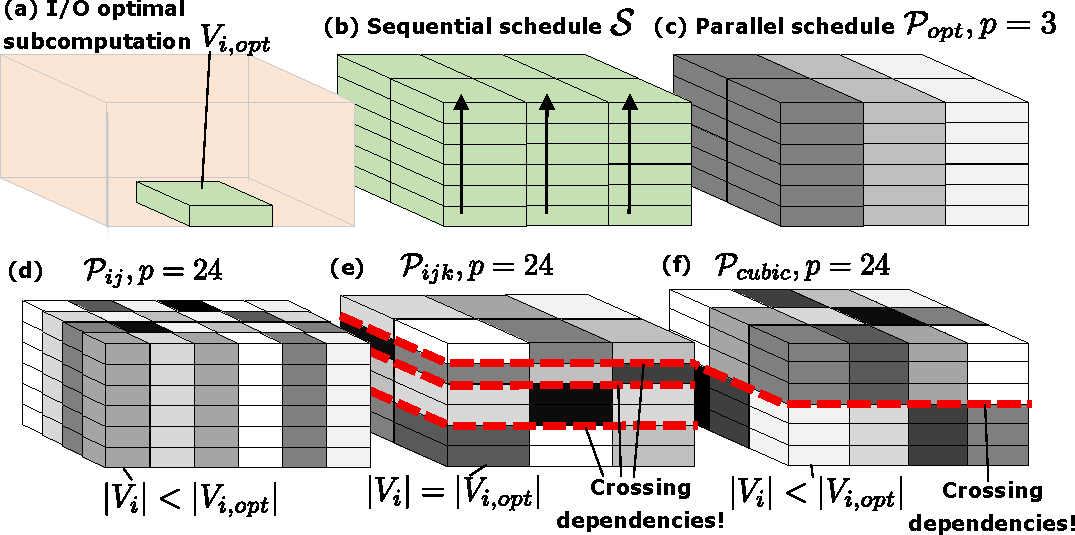
\includegraphics[width=\columnwidth]{figures/mmm_parallelization}
	\caption{Different parallelization schemes of I/O optimal sequential MMM 
	(3a). 
	Up to $p_1 = 6$ processes may 
		be 
		used without additional communication (3b). 
		Optimal 
		parallelization using $p=3$ processes (3c). 
		(3d-3f):  Parallelization strategies 
		using $p=24$ processes.} 
	\label{fig:mmmParallelization}
\end{figure}

When $p > p_1$, the size of local domains is reduced $\mathcal{D}_j < \sqrt{S} 
\times \sqrt{S} \times k $. There are two possibilities: first one is to 
parallelize in \textbf{k} dimension, breaking the data reuse and creating
dependencies between (resulting in additional communication, see
Figure~\ref{fig:mmmParallelization}e). The second possibility is to reduce the 
size of a domain in \textbf{ij} plane, not utilizing the whole available
memory, making the sequential schedule not I/O optimal and decreasing the
computational intensity $\rho$ (Figure~\ref{fig:mmmParallelization}d). We
  now analyze three possible parallelization
  strategies (Figure~\ref{fig:mmmParallelization}) that generalize 2D, 2.5D and 
  recursive decompositions' strategies:

%\mac{How about having a small table (one column) with various complexities of
%these following schedules?}
%\begin{enumerate}
%  \item \textbf{$\mathcal{P}ij$:} 

\macb{Schedule $\mathcal{P}ij$:} 
%
The schedule is parallelized in dimensions \textbf{i} and \textbf{j}. The
process grid is $[m/a , n/a, 1]$, where $a = \sqrt{\frac{mn}{p}}$.  Because all
dependencies are parallel to dimension \textbf{k}, there are no dependencies
between $\mathcal{D}_j$ except of the inputs and the outputs.  Because $a <
\sqrt{S}$, the corresponding sequential schedule $\mathcal{S}ij$ reduces the
computational intensity $\rho < \sqrt{S}/2$.

\macb{Schedule $\mathcal{P}ijk$}
%
The schedule is parallelized in all dimensions. The process grid is
$[m/\sqrt{S} , n/\sqrt{S}, mnk/(pS)]$.  The
computational intensity $\rho = \sqrt{S}/2$ is optimal. The parallelization in
\textbf{k} dimension creates dependencies between local domains, enforcing
communication and therefore increasing the I/O cost.

\macb{Schedule $\mathcal{P}cubic$} 
%
The schedule is parallelized in all dimensions. The process grid is $[m/a_c ,
n/a_c, mnk/a_c]$, where $a_c = \min\Big\{\big(\frac{mnk}{P}\big)^{1/3},
\sqrt{\frac{S}{3}}\Big\}$. Because $a_c < \sqrt{S}$, the corresponding
computational intensity $\rho < \sqrt{S}/2$.  Also,  the parallelization in
\textbf{k} dimension creates dependencies between local domains, introducing 
communication. 

\macb{Comparison with other algorithms: 
%	\mac{it could be combined in a
%suggested table, above}
}
%
If $m = n$, the $\mathcal{P}ij$ scheme is reduced to the classical 2D
decomposition (e.g., Cannon's algorithm~\cite{Cannon} or SUMMA~\cite{summa}).
If $m = n = k$, $\mathcal{P}ijk$ reduces to 2.5D decomposition~\cite{25d}.
Finally, CARMA~\cite{CARMA} asymptotically reaches $\mathcal{P}cubic$ scheme,
guaranteeing that the longest dimension of a local cuboidal domain is at most
two times larger than the smallest one. We present a detailed complexity 
analysis comparison for all algorithms in Table~\ref{tab:summary}.


\begin{table*}
	\vspace{-1em}
	%
	\setlength{\tabcolsep}{4pt}
	\renewcommand{\arraystretch}{1}
	\centering
	%\footnotesize
	\scriptsize
	\sf
	%
	\begin{tabular}{lllll}
		%
		\toprule
		%\vspace{-0.5em}
		%
		& \textbf{2D~\cite{summa}} & \textbf{2.5D~\cite{25d}} & 
		\textbf{recursive~\cite{CARMA}} & \textbf{COMM (this paper)} \\
		%
		\midrule
		%
		\makecell[l]{\textbf{process} %\\
			\textbf{decomposition} \\
			$\left[p_m \times p_n \times p_k\right]$}
		&
		$\left[\sqrt{p} \times \sqrt{p} \times 1\right]$
		&
		\makecell[l]{$\left[\sqrt{p/c} \times \sqrt{p/c} \times c\right]$; %\\
			$c = \frac{pS}{mk + nk}$}
		& 
		\makecell[l]{$\left[{2^{a_1}} \times {2^{a_2}} \times 
		{2^{a_3}}\right]$; %\\
			$a_1 + a_2 + a_3 = \log_2(p)$}
		& 
		\makecell[l]{$\left[\frac{m}{\sqrt{S}} \times \frac{n}{\sqrt{S}} \times 
			\frac{k}{d}\right]$; %\\
			$d = \frac{mnk}{pS}$}
		%
		%\vspace{1.0em}
		%
		\\
		%
		%\midrule
		%
		\textbf{domain size}
		&
		$\left[\frac{m}{\sqrt{p}} \times \frac{n}{\sqrt{p}} \times k\right]$ 
		&
		$\left[\frac{m}{\sqrt{p/c}} \times \frac{n}{\sqrt{p/c}} \times 
		\frac{k}{c}\right]$
		&
		$\left[\frac{m}{2^{a_1}} \times \frac{n}{2^{a_1}} \times 
		\frac{k}{2^{a_1}}\right]$
		& 
		$\left[{\sqrt{S}} \times {\sqrt{S}} \times {d}\right]$
		%
		%\vspace{0.5em}
		%
		\\
		\midrule
		%
		%\rowcolor{gray}
		\multicolumn{5}{c}{\textbf{``General case'':}} \\
		%\vspace{0.5em}
		%
		%\midrule
		%
		%   \makecell[l]{\textbf{``The easiest case'':}\\
		%   $m = n = k$,\\
		%   $S = 2\frac{n^2}{p}, p=2^{3n}$}
		%
		\textbf{I/O cost} $Q$
		&
		$\frac{1}{\sqrt{p}} \left(mk + nk\right)$
		&
		\makecell[l]{$(mk + nk)\sqrt{\frac{mn + mk + nk}{p^2S}} + \frac{MNS}{mn 
		+ mk + 
				nk}$; %\\
		} %$I = mn + mk + nk$}
		&
		\makecell[l]{$2\min \Big\{\sqrt{3} \frac{mnk}{p\sqrt{S}},
			\left(\frac{mnk}{P}\right)^{2/3} \Big\} $ %\\
			$ + \left(\frac{mnk}{P}\right)^{2/3}$}
		& 
		$\min \Big\{S + 2 \cdot \frac{mnk}{p\sqrt{S}}, 3 
		\left(\frac{mnk}{P}\right)^{2/3} \Big\}$
		%
		%\vspace{0.5em}
		%
		\\
		\textbf{latency cost} $L$
		&
		$2K/t$
		&
		to be filled
		&
		to be filled
		& 
		to be filled 
		\\
		%
		%\vspace{1.0em}
		%
		\midrule
		%
		%\rowcolor{gray}
		\multicolumn{5}{c}{\textbf{Square matrices, ``just enough memory'':} $m 
		= n = 
			k, S = 2{n^2}/{p}, p=2^{3n}$} \\
		%\vspace{0.5em}
		%
		%\midrule
		%
		%   \makecell[l]{\textbf{``The easiest case'':}\\
		%   $m = n = k$,\\
		%   $S = 2\frac{n^2}{p}, p=2^{3n}$}
		%
		\textbf{I/O cost} $Q$
		&
		${2N^2 }/{\sqrt{p}}$
		&
		${2N^2 }/{\sqrt{p}}$
		&
		$2N^2 \left(\sqrt{{3}/{2p}} + {1}/{2p^{2/3}} \right)$
		& 
		${2N^2 }/{\sqrt{p}}$
		%
		%\vspace{1.0em}
		%
		\\
		\textbf{latency cost} $L$
		&
		to be filled
		&
		to be filled
		&
		to be filled
		& 
		to be filled
		%
		%\vspace{1.0em}
		%
		\\
		%
		\midrule
		%
		%\rowcolor{gray}
		%\vspace{0.5em}
		\multicolumn{5}{c}{\textbf{``Tall'' matrices, ``extra'' memory 
		available:} $m = 
			n = \sqrt{p}, k = {p^{3/2}}/{4}, S = 2{nk}/{p^{2/3}}, p=2^{3n + 
			1}$} \\
		%
		%\midrule
		%
		%    \makecell[l]{\textbf{``the hardest case'':}\\
		%    $m = n = \sqrt{p}$,\\
		%    $k = \frac{p^{3/2}}{4}$,\\
		%    $S = 2\frac{nk}{p^{2/3}}, p=2^{3n + 1}$}
		%
		\textbf{I/O cost}
		&
		${p^{3/2}}/{2}$
		&
		${p^{4/3}}/{2} + p^{1/3}$
		&
		${3p}/{4}$
		& 
		$p\left({3-2^{1/3}}\right)/{2^{4/3}} \approx 0.69 p$
		%
		\\
		\textbf{latency cost} $L$
		&
		to be filled
		&
		to be filled
		&
		to be filled
		& 
		to be filled
		%
		%\vspace{1.0em}
		%
		\\
		%
		\bottomrule
		%
	\end{tabular}
	%
	\caption{The comparison of complexities of 2D, 2.5D, recursive, and COMM 
		algorithms. The 3D decomposition is a special case of 2.5D, and can be 
		obtained 
		by
		instantiating $c=p^{1/3}$ in the 2.5D case.
		%
		The most important symbols are described in Table~\ref{tab:symbols}. In 
		addition to the general analysis, we show two special cases. If the 
		matrices 
		are 
		square and there is no extra memory available, 2D, 2.5D and COMM 
		achieves tight 
		communication lower bound $2N^2/\sqrt{p}$, whereas CARMA performs 
		$\sqrt{3}$ 
		times more 
		communication. If one dimension is much larger than the others and 
		there is 
		extra memory available, 2D, 2.5D and CARMA decompositions perform 
		$\mathcal{O}(p^{1/2})$, $\mathcal{O}(p^{1/3})$, and 8\%  more 
		communication 
		than COMM, respectively. For simplicity, we assume that
		parameters are chosen such that all divisions have integer results.
		%
	}
	%
	\vspace{-2em}
	%
	\label{tab:summary}
\end{table*}

%\mac{It would be interesting to have some plot that shows a ``phase space''
%of these designs, with some points as 2D or 2.5D schemes, and your scheme
%as a ``region'' ?}

%-------------------------Old version starts here
%\greg{------------------ Old version starts here -------------------}
%

%In this section we show how to derive a communication optimal parallel 
%schedule 
%from the
%results derived in ~\cref{sec:seqScheduling}. The explicit notion of reuse 
%effects
%\mac{reuse affects?} not only sequential \mac{the sequential} execution, as
%discussed above, but also parallel scheduling \mac{the parallel scheduling}, as
%it determines data dependencies \mac{It's unclear why only affecting data
%dependencies have impact on the parallel schedule}.  Intuitively, the schedule
%consists of $mnk/S$ elementary outer product calculations, arranged in
%$\sqrt{S} \times \sqrt{S} \times k$ "blocks" (Figure
%\ref{fig:mmmParallelization}). The number of dependency-free subsets in the
%optimal S-partition determines the maximum degree of parallelism up to which no
%additional \mac{What does it mean ``additional''?} communication between
%processes is performed. Above this threshold, further parallelization requires
%either parallelizing dependent subsets \mac{How? Sounds very vague}, causing
%additional communication between processes, or by shrinking the size of
%subsets, reducing the effective memory size \mac{Why? And what is effective
%memory size?}.
%
%\macb{Note: shared vs distributed memory model}. \mac{``Note:'' sounds bad, 
%like
%you're writing some report as homework. Too unstructured. A paper must like the
%inside of a watch, everything strutured for one goal. No some weirdo ``notes''}
%%
%In our work we only evaluate the total data volume transfered \mac{This now
%sounds like you start Evaluation, but it's the algorithmic part - very
%confusing. Why?} \mac{``evaluate the total volume'' - sounds very limiting. It
%is stressed even more by adding: ``only'' - you're essentially telling yourself
%that the analysis here is very limited :)} (both horizontally and vertically).
%For distributed \mac{a distributed} machine \mac{Actually, instead of machine,
%I'd write ``For distributed environments'' - sounds better}, we assume that a
%network is fully connected \mac{All such assumtions should be a part of a
%separate section where the whole distirbuted setting is summarized and
%explained}. We furthermore omit the analysis of congestion or latency
%\mac{Without any citation and a brief statement that it's a common approach, it
%sounds like it sucks}. With those assumptions, our results hold for both shared
%and distributed memory machine \mac{machines? or even better, environments?} -
%one can view the former as the latter with $p + 1$ processes, where the
%$(p+1)$st process mimics the shared memory \mac{Huh? Completely unclear, how
%mimic? No reference to support, bad.} - it holds the initial data and performs
%no work \mac{No work? What does it mean? Also, suddenly work-depth is brough
%up? Extremely confusing}. To translate the shared memory results to a
%distributed machine, one needs to subtract the cost of transferring the initial
%data layout \mac{But you just swaid above that it ``mimics'' and one can view
%one as the other on some more processes - and now it's about some additional
%subtraction? Extremely confusing}. We note however, that this accounts for up
%to additive factor $(mk + nk)/p$ of total communication volume. \mac{Anyone is
%lost again here. All these statements above must be clarified, ordered, and
%placed in a separate section on distributed settings}
%
%We now analyze three possible parallelization strategies that trade I/O for 
%communication optimality \mac{Unclear what this means - trade I/O - put more
%details, and make it more precise - for example, ``increase the number of
%I/O operations in exchange for...''} (Figure~\ref{fig:mmmParallelization}):
%
%\begin{enumerate}
%  \item \textbf{par. in ij dim:} 
%  Parallelization is only on the \textbf{ij} plane \mac{Unclear, write more
%  precisely wht this means that parallelism is on some plane - actually,
%  this should be just mentioned in the associated background section on MM
%  (that parallelizing a given plane is paralelizing the corresponding 
%loop(s))}, therefore there is no 
%  reuse 
%  (no data sent) \mac{Such connections between the I/O and distributed world 
%  like reuse --- data sent should be gathered and explicitly discussed 
%somewhere I guess...} 
%  between the processes (communication optimality). The local domain size is 
%  $[a \times a \times k]$, where $a = \sqrt{\frac{mn}{P}} < \sqrt{S}$  (I/O 
%  optimality \mac{the I/O optimality} is broken \mac{Cars can be broken, 
%broken optimality sounds bad}).
%  \item \textbf{par. in ijk dim:} The subset's size is 
%  constant determined by 
%  Equation~\ref{eq:seqSolution} (I/O optimality). The 
%  parallelization is done 
%  in all 
%  three dimensions \mac{You sometimes mention parallelism in the context of 
%planes, and
%  sotimes dimentions - confusing}. The reuse crossing domains of parallel 
%processes in 
%  \textbf{k} 
%  requires sending data between them (communication optimality 
%  is broken).
%  \item \textbf{cubic} 
%  the local domain size is 
%  $[a_c \times a_c \times a_c]$, where $a_c = 
%  \min\Big\{\big(\frac{mnk}{P}\big)^{1/3}, 
%  \sqrt{\frac{S}{3}}\Big\}$ (both I/O and communication 
%  optimality is broken \mac{broken again}).
%\end{enumerate}
%
%\vspace{-3em}

\subsection{I/O Optimal Parallel Schedule}
\label{sec:parScheduling}

Observe that none of those schedules is optimal in the whole range of
parameters. As discussed in~\cref{sec:seqOpt}, in sequential scheduling, 
intermediate results of $C$ are not stored
to the memory: they are consumed (reused) immediately by the next
sequential step. Only the final result of $C$ in the local domain is sent.
Therefore, the optimal parallel schedule $\mathcal{P}_{opt}$ minimizes the
communication, that is, sum of the inputs' sizes plus the output size, under
the sequential I/O constraint on subcomputations $\forall_{V_i \in
\mathcal{P}_{opt}} |Dom(V_i)| \le S \land |Min(V_i)| \le S$.

The local domain $\mathcal{D}_j$ is a cuboid of size $[a \times a \times b]$. 
The optimization problem of finding $\mathcal{P}_{opt}$
using the 
computational intensity (~\cref{sec:iolowerbounds}) can be 
formulated as 
follows:
%\vspace{-1em}
\begin{gather}
\label{eq:tileEq}
\nonumber
\text{maximize } \rho = \frac{a^2b}{ab + ab + a^2}\\
\nonumber
\text{subject to: } \\
\nonumber
a + a + a^2 \le S \text{ (the I/O constraint)} \\
\nonumber
a^2b = \frac{mnk}{p} \text{ (the load balance constraint)} \\
a, b, m, n, k, p, S \in \mathbb{Z}_{> 0}
\end{gather}
%\vspace{-1em}
where $p$ is the number of processes. The I/O constraint $2a + 
a^2 \le 
S$ is tight (binding) for $p \ge \frac{mnk}{S^{3/2}}$. Therefore, the solution 
to this problem (using the 
approximation $\sqrt{S+1} - 1 \approx \sqrt{S}$):
%\vspace{-1em}
\begin{gather}
\nonumber
a = \min\Big\{\sqrt{S}, \Big(\frac{mnk}{p}\Big)^{1/3} \Big\}\\
b = \max\Big\{\frac{mnk}{pS}, \Big(\frac{mnk}{p}\Big)^{1/3} \Big\}
\label{eq:optTileShape}
%\end{cases}\\
\end{gather}
%\vspace{-1em}
\noindent
This can be intuitively interpreted geometrically as follows: if we 
imagine the 
optimal local domain "growing" with the decreasing number of processes, 
then it is 
cubic until it is still "small enough" (its side is smaller than 
$\sqrt{S}$). 
After that point, its face in \textbf{ij} plane stays constant 
$\sqrt{S} \times 
\sqrt{S}$ and it "grows" 
only in the \textbf{k} dimension. This schedule effectively switches 
from $\mathcal{P}ijk$ to $\mathcal{P}cubic$ once there is enough 
memory ($S \ge \big(\frac{mnk}{p}\big)^{2/3}$).

\begin{lma}
  \label{lma:parSchedule}
  Parallel schedule $\mathcal{P}_{opt} = \{\mathcal{D}_j\}$ composed of $p$ 
  local domains $\mathcal{D}_j$ of size 
  determined by Equation~\ref{eq:optTileShape} is asymptotically 
  communication optimal, that is, the communication volume is minimal across 
  all parallel schedules $\mathcal{P}$ with $p$ processes.
\end{lma}

\begin{proof}
The communication cost $Q$ of each local domain $\mathcal{D} \in 
\mathcal{P}_{opt}$ is the sum of communication costs of all subcomputations 
$V_i 
\in \mathcal{D}$. Each subcomputation $V_i$ requires $2a$ elements to be 
communicated (~\cref{sec:seqOpt}). The number of subcomputations is 
$|\mathcal{D}| = b$. Furthermore, the last subcomputation $V_b$ must 
communicate $a^2$ outputs. Therefore, the total communication cost $Q$ 
is: 
%the sum of communications of all processes:
\vspace{-1em}

$$Q = \max\Big\{\frac{2mnk}{\sqrt{S}} + 
S, 3\Big(\frac{mnk}{p}\Big)^{2/3}  \Big\}$$

This schedule is asymptotically communication optimal, as it reaches both 
memory-dependent and 
memory-independent lower bound~\cite{memIndependentBound}.
\end{proof}


\subsubsection{I/O-Latency Trade-off}
\label{sec:latencyTradeoff}
As showed in~\cref{sec:parScheduling}, the local domain $\mathcal{D}$ of the 
I/O optimal 
schedule $\mathcal{P}$ is a cuboid of size $[a \times a \times b]$, where $a, 
b$ are given by Equation~\ref{eq:optTileShape}. The I/O cost of each  
$\mathcal{D}$ is $2ab$ (size of the inputs) plus $a^2$ (output). 
 The corresponding sequential 
schedule $\mathcal{S}$ is a sequence of $b$ outer products of vectors of length 
$a$. Denote the size of the required inputs in each step by $I_{step} = 2a$. 
However, this corresponds to $b$ steps of communication ($L = b$).

The number of steps (latency) is equal to the communication volume divided by 
the volume per step $L = Q/I_{step}$. To reduce the latency, one 
either have to decrease $Q$ or increase $I_{step}$, under the memory 
constraint that $I_{step} + a^2 \le S$ (otherwise we cannot fit the inputs and 
the outputs in the memory). Express $I_{step} = a \cdot h$, where $h$ is the 
number of sequential subcomputations $V_i$ we merge in one communication. We 
can now express the I/O-latency trade-off:
\vspace{-0.5em}
\begin{gather}
\nonumber
Q = 2ab + a^2 \\
\nonumber
L = \frac{b}{h} \\
\nonumber
a^2 + 2ah \le S \text{ (I/O constraint)} \\
\nonumber
a^2b = \frac{mnk}{p} \text{ (load balance constraint)}
\end{gather}
Solving this problem, we have $Q = \frac{2mnk}{pa} + a^2$ and $L 
= 
\frac{mnk}{pa(S-a^2)}$, 
where $a \le \sqrt{S}$. Increasing $a$ we \emph{reduce} I/O cost 
$Q$ and \emph{increase} latency cost $L$. For minimal value of 
$Q$ (Lemma~\ref{lma:parSchedule}),  $L = \left \lceil{\frac{2ab}{S - 
a^2}}\right\rceil$, where $a = \min\{\sqrt{S}, (mnk/p)^{1/3} \}$ and \linebreak 
$b = 
\max\{\frac{mnk}{pS}, (mnk/p)^{1/3} \}$. Based on our 
experiments, we observe that the I/O cost is vastly greater than the 
latency cost, therefore our schedule by default minimizes $Q$ and uses 
extra memory (if any) to reduce $L$. However, we leave that as a tunable 
parameter dependent on the hardware parameters.

%
%\subsubsection{Parallel efficiency} 
%
%We now proceed to analyze the 
%communication's 
%\emph{parallel efficiency} of all parallelization schemes. We define it as a 
%ratio between  
%the total data movement required by the sequential processor (Theorem 
%\ref{thm:seqlowbounds}) and sum of data movements performed by all 
%parallel
%processes. More 
%formally, if $Q(p,S)$ is the data movement cost per process of the 
%algorithm 
%using $p$ 
%processes, each of local fast memory size $S$, then the parallel 
%efficiency 
%metric for communication is defined as $E(p,S) = 
%\frac{Q(1,S)}{pQ(p,S)}$.
%
%In the proof of Lemma~\ref{lma:parSchedule} we derive $pQ(p,S)$ for 
%$\mathcal{P}Copt$. Using the same technique, we obtain $pQ(p,S)$ for the 
%remaining schedules $\mathcal{P}ij$, $\mathcal{P}ijk$, and $\mathcal{P}cubic$.
%The results of our analysis is shown in Table \ref{tab:mmmEfficiency} 
%and 
%Figure \ref{fig:mmmScaling}.
%
%
%\begin{table*}[t]
%  \begin{tabular}{lllll}
%    \toprule
%    range & metric & par in \textbf{ij} dim & par. in 
%    \textbf{ijk} dim & 
%    cubic \\
%    \midrule 
%    %
%    \multirow{3}{*}{$p \le \frac{mn}{S}$}
%    %
%    & loc. dom. & $[\sqrt{S} \times \sqrt{S} \times k]$ & 
%    $[\sqrt{S} 
%    \times \sqrt{S} \times k]$ & $\Big[\sqrt{\frac{S}{3}} \times 
%    \sqrt{\frac{S}{3}} \times \sqrt{\frac{S}{3}}\Big]$ \\
%    \cline{2-5}
%    %
%    & $pQ(p,S)$ & 
%    $\frac{2mnk}{\sqrt{S}} + mn$ & 
%    $\frac{2mnk}{\sqrt{S}} + mn$ & 
%    $\frac{3\sqrt{3}mnk}{\sqrt{S}}$ \\
%    \cline{2-5}
%    %
%    & $E(p,S)$ & 1 & 1 &   $\frac{2K + 
%    \sqrt{S}}{3\sqrt{3}k}$ \\
%    \midrule 
%    %
%    \multirow{3}{*}{
%      \begin{tabular}{l}
%        $\frac{mn}{S} < p$ \\
%        $p \le \Big(\frac{3}{S}\Big)^{3/2}mnk$
%      \end{tabular}     
%    }
%    % 
%    & loc. dom. & $\Big[\sqrt{\frac{mn}{p}} \times 
%    \sqrt{\frac{mn}{p}} 
%    \times k\Big]$ & $\Big[\sqrt{S} 
%    \times \sqrt{S} \times \frac{mnk}{Sp}\Big]$ & 
%    $\Big[\sqrt{\frac{S}{3}} 
%    \times 
%    \sqrt{\frac{S}{3}} \times \sqrt{\frac{S}{3}}\Big]$ \\
%    \cline{2-5}
%    %
%    & $pQ(p,S)$ & $2K 
%    \sqrt{pmn} + mn$ & 
%    $\frac{2mnk}{\sqrt{S}} + pS$ & 
%    $\frac{3\sqrt{3}mnk}{\sqrt{S}}$ 
%    \\
%    \cline{2-5}
%    %
%    & $E(p,S)$ & $\frac{mnk(\frac{2}{\sqrt{S}} + 
%    \frac{1}{k})}{2K\sqrt{MNp} 
%    + mn}$ & $\frac{2mnk(1 + \frac{\sqrt{S}}{2K})}{2mnk + 
%    S^{3/2}p}$ &   
%    $\frac{2K + 
%      \sqrt{S}}{3\sqrt{3}k}$ \\
%    \midrule \\
%    %
%    \multirow{3}{*}{$p > \Big(\frac{3}{S}\Big)^{3/2}mnk$}
%    %
%    & loc. dom. & $\Big[\sqrt{\frac{mn}{p}} \times 
%    \sqrt{\frac{mn}{p}} 
%    \times k\Big]$ & $\Big[\sqrt{S} 
%    \times \sqrt{S} \times \frac{mnk}{Sp}\Big]$ & 
%    \begin{tabular}{l}
%$\Big[a 
%\times 
%a \times 
%a\Big]$ \\
%$a = \big(\frac{mnk}{p}\big)^{1/3}$
%    \end{tabular} 
%  \\
%  \cline{2-5}
%    %
%    & $pQ(p,S)$ & $2K 
%    \sqrt{pmn} + mn$ & 
%    $\frac{2mnk}{\sqrt{S}} + pS$ & 
%    $3p\big(\frac{mnk}{p}\big)^{2/3}$ 
%    \\
%    \cline{2-5}
%    %
%    & $E(p,S)$ & $\frac{mnk(\frac{2}{\sqrt{S}} + 
%    \frac{1}{k})}{2K\sqrt{MNp} 
%      + mn}$ & $\frac{2mnk(1 + \frac{\sqrt{S}}{2K})}{2mnk + 
%      S^{3/2}p}$ &   
%    $\frac{2mnk(1 + 
%    \frac{\sqrt{S}}{2K})}{3p^{1/3}\sqrt{S}(mnk)^{2/3}}$ \\
%  \end{tabular}
%  \caption{Total communication volume of MMM and its parallel 
%  efficiency of 
%  the 
%  different parallelization schemes. We assume that all the 
%  respective local 
%  domain sizes divide the global matrix sizes evenly (e.g., for 
%  cubic domain 
%  in range $p \le mn/S$, we assume that $\sqrt{S/3} = a_1M = a_2N = 
%  a_3K$ for 
%  $a_1, a_2, a_3 \in \mathbb{N}$). The optimal schedule 
%  (\cref{sec:parScheduling}) switches from \textbf{par. in ijk} to 
%  \textbf{cubic} when $p \ge \frac{mnk}{S^{3/2}}$.}
%  \label{tab:mmmEfficiency}
%\end{table*}
%
%
% \begin{figure*}[t]
%     \centering
%   %
%   \hspace{-1cm}
%   \subfloat["flat" matrices]{\includegraphics[width=0.33\textwidth]
%     {figures/efficiencyPlot11}\label{fig:effic1}}
%   %
% %\hfill
%   %
%   \subfloat[square matrices, small 
%   $S$]{\includegraphics[width=0.33\textwidth]
%     {figures/efficiencyPlot12}\label{fig:effic2}}
%   %
%  %\hfill
%   %
%   \subfloat[square matrices, large 
%   $S$]{\includegraphics[width=0.33\textwidth]
%     {figures/efficiencyPlot13}\label{fig:effic3}}
%   %
%   \hspace*{-1.5cm}
%   \caption{Parallel 
%   efficiency 
%   of different parallelization schemes. Three vertical dashed lines 
%   correspond to 
%     thresholds 
%     $p1 = mn/S$, $p2 = mnk/S^{3/2}$ and $p3 = 
%     (\frac{3}{S})^{3/2}mnk$ (Table \ref{tab:mmmEfficiency}). Note 
%     that for cases (b) and (c), increasing memory $S$ six times 
%     reduces the number of processes required to fully saturate it 
%     drops from $p2=741455$ to $p2=50449$. }
%   \label{fig:mmmScaling}
% \end{figure*}

\section{Implementation}
\label{sec:implementation}
We now present implementation optimizations that further 
increase the performance of COMM on top of the speedup due to our I/O optimal 
schedule. The algorithm is designed to facilitate the overlap of computation 
and communication~\cref{sec:compOverlap}. For this, to leverage the RDMA 
mechanisms of 
current high-speed network interfaces, we use the MPI one-sided 
interface~\cref{sec:rdma}. In addition, our implementation also offers 
alternative efficient two-sided communication backed that uses MPI collectives. 
We also use a block-cyclic data 
layout~\cref{sec:datalayout}, a grid-fitting 
technique~\cref{sec:decompArbitrary} and an optimized binary broadcast 
tree using static information about
the communication pattern~\cref{sec:commPattern} together with the buffer 
swapping~\cref{sec:bufferReuse}. For the local matrix operations, we use 
BLAS routines for highest performance. Together, those optimizations account 
for \greg{Missing} total runtime 
reduction. 

\subsection{Blocked Data Layout}
\label{sec:datalayout}
COMM schedule specifies what input data is required by each processes
independently of the initial data distribution. 
Therefore, having $c$ initial redundant copies of $A$ and $B$ reduce the 
communication up to $\sqrt{p}/(\sqrt{p} - c)$ times: if we allow $c = \sqrt{p}$ 
copies, then COMM does not require any communication at all. However, in 
practice we usually 
assume that $c=1$. In this 
case, COMM schedule induces the optimal initial data 
layout, since it specifies for each subset $I$ of a input matrices $A$ and $B$, 
which 
processes $\left\{ p_1, ... p_x\right\}$) requires it. 
However, the schedule does not specify how to distribute subsets $I$ further 
among these processes. Here we go a step further: we first split each of $I$ 
into $x$ smaller blocks $I_1, ... I_x$ and then aim to assign each 
block to a single process from $\left\{ p_1, ... p_x\right\}$ such that the 
data movements during communication are minimized. We achieve this by enforcing 
that consecutive blocks are assigned to processes that communicate first. By 
finding a mapping between processes and blocks that resembles the 
communication schedule, we guarantee that after each communication round, each 
process owns a consecutive block of initial matrix without any need of local 
data reshuffling. This property of owning a consecutive pieces of matrix is 
hence preserved both before and after each communication. This is unlike the 
distributed CARMA implementation~\ref{carma}, which uses the cyclic 
distribution among processes in the recursion base case and requires local data 
reshuffling after each communication round. Another advantage of our blocked 
data layout is a full compatibility with the block-cyclic data 
layout, that can be seen in e.g. ScaLAPACK. This offers a compatibility 
of our algorithm with other linear-algebra libraries.


\subsection{Process Grid Optimization}
\label{sec:decompArbitrary}
\begin{figure}[!tbp]
	\centering
	%
	\subfloat[$1 \times 3 \times 15$ 
	grid]{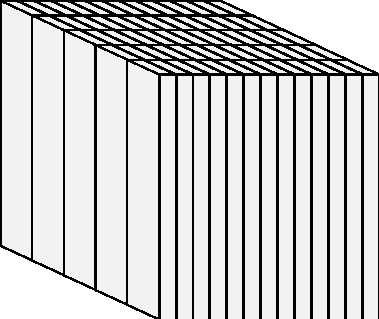
\includegraphics[width=0.18\textwidth]
		{figures/proc_decomp_problem_bad}\label{fig:decomp_left}}
	%
	\hfill
	%
	\subfloat[$4 \times 4 \times 4$ grid with one idle 
	process]{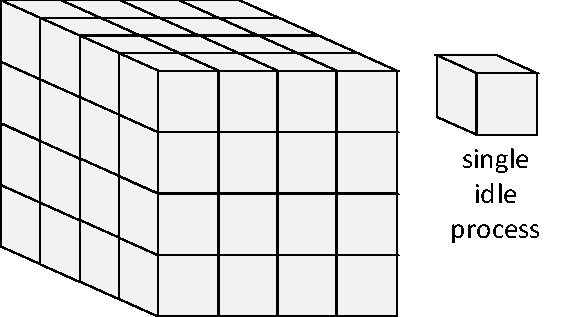
\includegraphics[width=0.27\textwidth]
		{figures/proc_decomp_problem_good}\label{fig:decomp_right}}
	%
	\caption{Process decomposition for square matrices and 65 
		processes. To utilize all resources, the local domain is 
		drastically stretched (a). Dropping one 
		process results in a symmetric grid (b) that 
		increases the computation per process only by 1\%, but reduces 
		the communication by 36\%.}
	\label{fig:decompProblem}
\end{figure}
Throughout the paper, we assume all operations required to 
assess the decomposition (divisions, roots, powers) result in natural 
numbers. We note that in practice it is rarely the case. E.g., the 
domain emerging from an exemplary 
water molecule simulation~\cite{joost}, when launched on the whole 
Piz Daint supercomputer with 1813 nodes, cannot be equally decomposed. 
Moreover, the memory size per 
node (64~GiB DDR, 90~MiB L3 cache) does not give the integer solution 
for the local domain size $a = \sqrt{S+1} -1$. One may use the straightforward 
approach to take  
the floor and ceiling
functions for non-natural numbers, but this may result in suboptimal 
results, as we demonstrate in the following example.

Assume that we multiply two square matrices with 65 
processes (Figure~\ref{fig:decompProblem}). We choose 65 as it easily 
visualizes our key observation here, but any number which is divisible by 
relatively large primes ($>11$) serves the case).
  The only integer factors 
of 65 are 1, 5 and 13. Therefore, to 
utilize all the resources, the processes must be arranged in a $[13 
\times 5 \times 1]$ grid (up to a permutation). On the other hand, if 
we decide \emph{not to utilize all resources} 
and drop one process, then we can arrange remaining 64 in a $[4 
\times 4 \times 4]$ grid. Such an arrangement \emph{trades communication 
	for computation:} it increases the number of arithmetic operations 
per process by 1\%, while decreasing the communication volume per 
process by 36\%. However, because the dense MMM is compute bound, the 
decision which arrangement is better is not obvious.
% In this extreme example the trade-off is clearly visible, but 
%In most real life scenarios it is a non-trivial decision 
%and depends on the computation and communication performance of a 
%machine. 
In most real life scenarios this trade-off may vary and the optimal 
decomposition depends on the computation and communication 
performance 
of a 
machine. 


%This gives $2.15\cdot10^9$ arithmetic operations 
%(only 1\% increase) and $3\cdot10^6$ elements communicated (36\% 
%decrease).
%This results in 
%$2.12\cdot10^9$ arithmetic operations and approx. $5\cdot10^6$ 
%elements communicated per process.

The existing algorithms cannot handle such case (CARMA), 
require a user to manually specify the decomposition (ScaLAPACK), or 
consider only the decompositions that utilize all processes
(CTF). Our algorithm balances this computation--communication 
trade-off by "stretching" the local domain size 
derived in ~\cref{sec:parScheduling} to fit the global 
domain by adjusting its width, height and length. The range of this 
tuning (how far the shape of the local domain is from the optimal one, 
increasing communication but utilizing more resources) 
depends on the hardware specification of the 
machine (peak FLOPS, memory and network bandwidth). For our 
experiments on Piz Daint we chose the maximal ratio between the 
optimal and applied size to be \greg{Missing}, accounting for up to 
\greg{Missing} speedup.

\subsection{Enchanced Communication Pattern}
\label{sec:commPattern}
As shown in Algorithm~\ref{alg:comm}, COMM by default executes in $t = 
\frac{2ab}{S - a^2}$ 
rounds. In each round, each process receives $s = ab/t = (S - a^2)/2$ 
elements of 
$A$ 
and 
$B$. Thus, the input matrices are broadcast among the \textbf{i} and \textbf{j} 
dimensions of the process grid. After the last round, the partial results of 
$C$ 
are reduced among the \textbf{k} dimension. The communication pattern is 
therefore similar to ScaLAPACK or CTF.

To accelerate the collective communication, we implement our own binary 
broadcast 
tree, taking advantage of a known data layout, process grid, and communication 
pattern.
 Knowing the initial data 
layout~\cref{sec:datalayout} and the process 
grid~\cref{sec:decompArbitrary}, we craft the binary reduction tree 
in all three dimensions \textbf{i}, \textbf{j} and \textbf{k} such that a 
distance in the grid between communicating processes is minimized. 

Given a $[g_M, g_N, g_K]$ process grid, we organize processes 
in a balanced binary tree with $g_i$ leaves ($i \in \{m,n,k\}$) in each 
dimension. The 
communication 
(either distributing inputs $A$ and $B$, or reducing output $C$) is performed 
in 
$\left \lceil{log_2(g_i)} \right \rceil$ steps, sending data of size $2^{r-1} 
D$, where $r$ is the step 
number, and $D$ is the local size of data to be distributed.

\subsection{Computation--Communication Overlap}
\label{sec:compOverlap}
The sequential rounds of the algorithm $t_i = 1, \dots, t$, 
naturally express 
computation--communication overlap. Using double buffering, at each round $t_i$ 
we issue an asynchronous communication (using either MPI\_Put or 
MPI\_Isend / MPI\_Irecv~\cref{sec:rdma}) of the data required at round 
$t_{i+1}$, 
while locally processing the data received in a previous round. We note that, 
by the construction of the local domains 
$\mathcal{D}_j$~\cref{sec:parScheduling}, the extra memory required for double 
buffering is rarely an issue. If we are constrained by the available memory, 
then the space required to hold the partial results of $C$, which is $a^2$, is 
much larger than the size of the receive buffers $s =(S - 
a^2)/2$. If not, then there is extra memory available for the buffering.

\macb{Number of rounds:} The minimum number of rounds, and therefore minimum 
latency, is $t= \frac{2ab}{S-a^2}$~\cref{sec:latencyTradeoff}. However, to 
exploit more computation--communication overlap, we can increase 
the number of rounds $t_2 > t$. In this way, in one round we communicate less 
data $s_2 = ab/t_2 < s$, allowing the first round of computation to start 
earlier.

\subsection{One-Sided vs Two-Sided Communication}
\label{sec:rdma}
To reduce the latency~\cite{fompi} we implemented communication 
using MPI RMA~\cite{mpi3-rma-overview}. This interface utilizes the 
underlying features of Remote Direct Memory Access (RDMA) mechanism, bypassing 
the OS on the receiver side and providing zero-copy communication: data sent is 
not buffered in a temporary address. Instead, it is written directly to its 
location).

All communication windows are 
pre-allocated using \linebreak MPI\_Win\_Allocate with the size of maximum 
message in the 
broadcast tree $2^{s-1} D$~\cref{sec:commPattern}. Communication in each 
step is performed using MPI\_Put with passive synchronization (MPI\_Lock / 
MPI\_Unlock).

For compatibility reasons, as well as for the performance comparison, we also 
implemented a communication back-end using MPI two-sided (the message passing 
abstraction). In our tests on Piz Daint, we observed that the two-sided version 
was \greg{Missing} faster/slower than the one-sided one.


\subsection{Communication Buffer Optimization}
\label{sec:bufferReuse}
The used binary broadcast tree pattern is a generalization 
of 
the recursive structure of CARMA. However, CARMA in each step of the 
recursion dynamically allocates new buffers of the increasing size to match the 
message sizes $2^{s-1} D$, causing an additional runtime overhead.

To alleviate this problem, we pre-allocate a 
single buffer per matrix A, B and C of the maximum size of the message $ab/t$, 
where $t = \frac{2ab}{S - a^2}$ is the number of steps in COMM 
(Algorithm~\ref{alg:comm}). Then, in each level $s$ of the communication tree, 
we  move the pointer in the receive buffer by $2^{s-1} D$ elements.

%We offer two versions of the algorithm: an \emph{asynchronous} 
%version using the one-sided communication backend and a 
%\emph{synchronous} version using the two-sided communication. The 
%choise of the version to be used can be made at the runtime of the 
%algorithm. In the asynchronous version, each rank has a read-only 
%buffer that holds the initial data and the data from this buffer can 
%be fetched by any processor at any time without any synchronization 
%between processors. This allows a natural separation of the logic 
%behind the initial data layout and the computation: what a processor 
%computes as the output might be independent of what data this 
%processor initially owns, thus allowing an overlap of communication 
%and computation. The drawback of this approach is that a processor 
%cannot use this initial buffer, they are read-only and they only 
%serve to allow the access to this data for any process that might 
%need it. In the two-sided version, the communication happens in 
%synchronously: whenever a processor has to compute some subproblem, 
%it will first collect all the necessary input data and then perform 
%the computation. Here, instead of always exchanging just the content 
%of the \emph{initial}, read-only buffers (as in the one-sided 
%version), the processors exchange the content of the current, 
%\emph{working} buffers, which they also actively use. For this 
%reason, we want to avoid the need of local data reshuffling in these 
%\emph{working} buffers which might be needed after the communication. 
%This can be achieved by carefully corellating the initial data layout 
%with the order of the data exchanges throughout the algorithm, which 
%is explained in the next section. 
%
%\greg{We use two buffers instead of $\log P$}

\section{Evaluation}
\label{sec:evaluation}

We evaluate COMM against other state-of-the-art implementations with various 
combinations of matrix dimensions and memory requirements. These scenarios 
include both synthetic square matrices, in which all algorithms achieve their 
peak performance, as well as real-world "tall-and-skinny" cases with uneven 
numbers of available processes. 
 
%\mac{My papers, for example, RMA Locks or Push Pull, or Slim NoC,
%contain good Evaluation sections, I'd suggest checking them in case
%of some doubts}

\macb{Comparison Targets}
%
As a comparison, we use the widely used ScaLAPACK library (commit number 
3287fdd 
on May 17, 2018), as well 
as Cyclops Tensor Framework (commit number 6aaf037 on February 16, 2018), and 
the original CARMA implementation (commit number 7589212 on July 19, 2013).

%\macb{Datasets}
%%
%\mac{What concrete datasets are used?}
\macb{Matrix Dimensions and Number of Processes}
We use both square ($m = n = k$) and "skinny" ($m = n \ll k$) matrices. Due to 
space constraints, we skip the ``flat'' case (e.g., $m \ll n = k$) as being 
``in between'', and limit 
ourselves to these two representative cases. The matrix dimensions and number 
of 
processes are (1) powers of 
two $m = 2^{r_1}, n = 2^{r_2}, m = 2^{r_3}$, (2) determined by the real-life 
simulations or hardware architecture (available nodes on a computer), (3) 
chosen adversarily, e.g, $n^3 + 1$. 
Skinny matrix dimensions were taken from an application benchmark, namely the 
calculation of the random phase approximation (RPA) energy of water 
molecules~\cite{joost}. There, to simulate $w$ molecules, the sizes 
of the 
matrices are $m=n=136w$ and $k = 228w^2$. We use $w=64$ as in the 
original paper, yielding $m=n=8704, k = 933888$.

\macb{Selection of Benchmarks}
%
We perform both strong scaling and \emph{memory scaling} experiments. 
The memory scaling scenario fixes the input size per process 
($\frac{pS}{I}, I = mn + mk + nk$), as opposed to the work per 
process ($\frac{mnk}{p} \ne const$). We evaluate two cases: (1) "just enough 
memory" ($\frac{pS}{I} = 1$), and (2) "extra memory"  ($\frac{pS}{I} = 
p^{1/3}$).
%
%\mac{Instead of this list, I'd suggest use a block of text (list in text)
%like in my Push Pull paper or in RMA Locks paper}
%%
%We chose our experiments to cover the whole spectrum of possible use 
%cases. We 
%compare
%\begin{itemize}
%  \item square ($m=n=k$) vs "skinny" ($m=n << k$) matrices,
%  \item different memory requirements: just enough memory to fit 
%  the inputs 
%  ($S = (mk + nk)/p$) vs enough memory for $p^{1/3}$ redundant 
%  copies of data,
%  \item weak vs strong scaling,
%  \item parameter values that are powers of two vs randomly chosen 
%  vs 
%  determined by real-life problem definition.
%\end{itemize}
%
%For our "skinny" matrix, as a use case we evaluate the problem of 
%water 
%molecules interaction in the DFT
%simulation\cite{joost}. There, to simulate $w$ molecules, the sizes 
%of the 
%matrices are $m=n=136w$ and $k = 228w^2$. We use $w=64$ as in the 
%original paper, yielding $m=n=8704, k = 933888$.
%
%\macb{Varied Parameters}
%%
%\mac{Are there any additional important parameters to be explicitly described?}

\macb{Programming Models}
%
As stated in~\cref{sec:rdma}, we use both the RMA and the Message Passing 
models. CTF also uses both models, whereas CARMA and ScaLAPACK use MPI 
two-sided (Message Passing).

\macb{Experimentation Methodology}
%
For each combination of parameters, we perform 20 runs. As all the algorithms 
use BLAS routines for local matrix computations, we discard the first run due 
to the BLAS setup overhead. We report median and 95\% confidence intervals of 
the runtimes.
%\mac{How is data gathered? What is considered? Info on statistical measures,
%confidence intervals, other statistical info}

\macb{Experimental Setup and Architectures}
%
We run our experiments on the CPU partition of the CSCS Piz Daint, which has 
1813 XC40 nodes with
dual-socket Intel Xeon E5-2695 v4 processors (3.30 GHz,45 MiB L3 shared cache, 
64 GiB DDR3 RAM),
interconnected with Cray Aries network.

\macb{Infrastructure and Implementation Details}
%
All implementations were compiled using the gcc 5.3.0 compiler with the -O3 
flag. We use 
Cray-MPICH 3.1 implementation of MPI. The intra-node parallelism is handled 
internally by the MKL BLAS version 2017.4.196. 
%\mac{Any information about, for example, version of MPI used, and/or
%things like PAPI, OpenMP? Also versions of used compilers, etc.}

\section{Results}
\label{sec:results}
We now present the experimental results comparing COMM with the existing 
algorithms. For each of the scenarios: strong, memory and size scaling, we test 
the runtime on both square and skinny matrices. As can be seen, COMM is always 
the fastest in \emph{all} scenarios. 
Furthermore, due to the process grid optimization~\ref{sec:decompArbitrary}, 
the performance is stable and does not suffer from bad combinations of 
parameters. For example, the total runtime of COMM for square matrices $m=n=k=$ 
\greg{Missing} on $p_1=$ \greg{Missing} is \greg{Missing}. Increasing number of 
processes to $p_2=$ \greg{Missing} reduces the runtime to \greg{Missing}. On 
the other hand, CTF for $p_1$ runs in \greg{Missing}, while for $p_2$ the 
runtime \emph{increases} to \greg{Missing}.

\subsection{Strong Scaling}
\macb{Square Matrices} In this scenario we fix the matrix sizes to $m=n=k=$ 
\greg{Missing}. 
\begin{figure}
	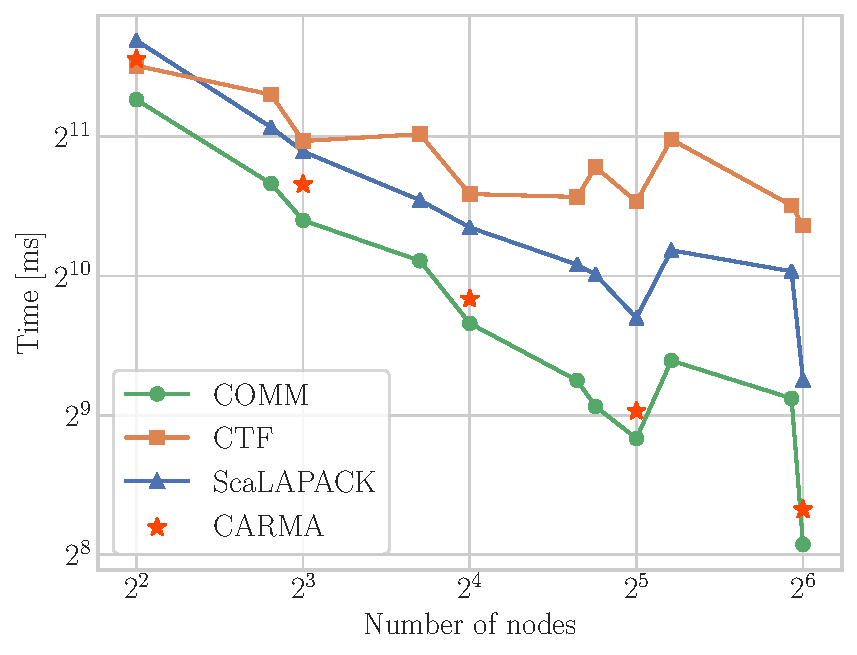
\includegraphics[width=\columnwidth]{results/square_strong_scaling}
	\caption{Square matrices, strong scaling. $n=m=k=$ \greg{Missing}} 
	\label{fig:mmmParallelization}
\end{figure}

\noindent
\macb{"Skinny" Matrices} Here we use the matrices used to simulate 
\greg{Missing} water molecules in the RPA scheme, resulting in $m=n=$ 
\greg{Missing}, and $k=$ \greg{Missing} 
\greg{Missing}. 
\begin{figure}
	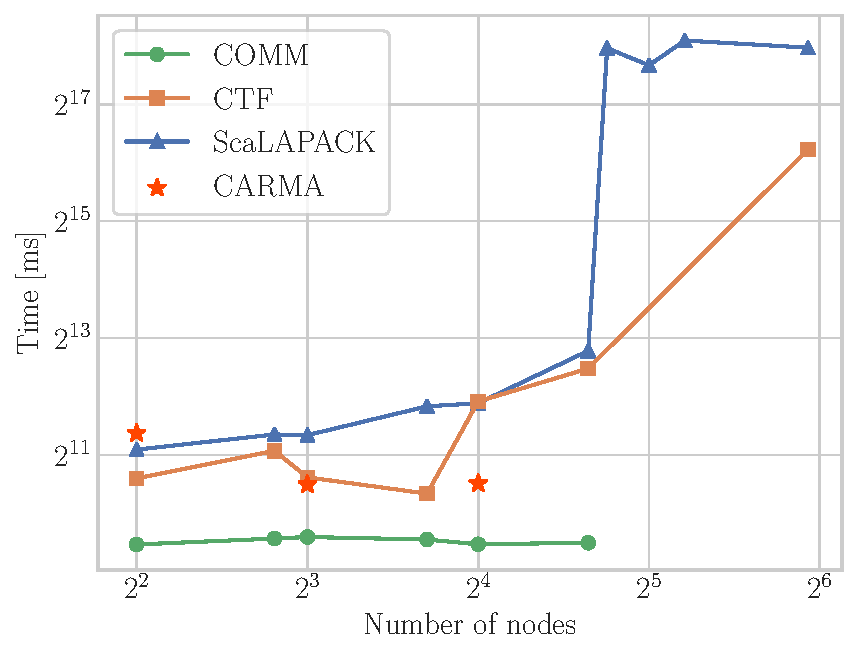
\includegraphics[width=\columnwidth]{results/thin_strong_scaling}
	\caption{"Skinny" matrices, strong scaling. $n=m=$ \greg{Missing}, $k=$ 
	\greg{Missing}} 
	\label{fig:mmmParallelization}
\end{figure}

\subsection{Memory Scaling}
For those tests, we scale the problem size so that the size of the input 
remains either constant $\frac{pS}{I} = 3$ (for ``just enough memory'' case) or 
to maintain a fixed replication factor $\frac{pS}{I} = p^{1/3}$.

%\macb{Square Matrices}
\begin{figure}
	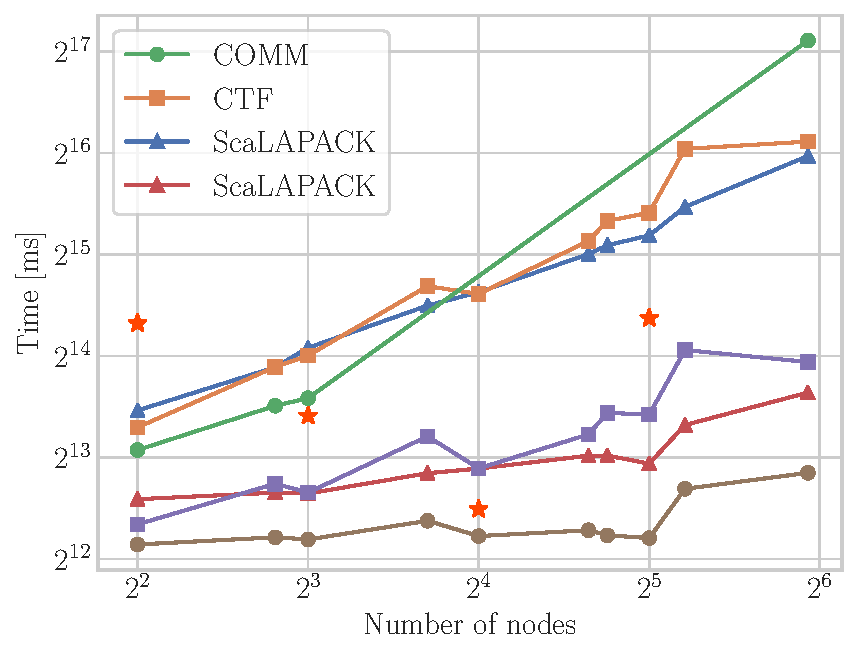
\includegraphics[width=\columnwidth]{results/square_weak_scaling}
	\caption{Square matrices, memory scaling. $n=m=k=$ \greg{Missing}} 
	\label{fig:mmmParallelization}
\end{figure}

%\macb{"Skinny" Matrices}
\begin{figure}
	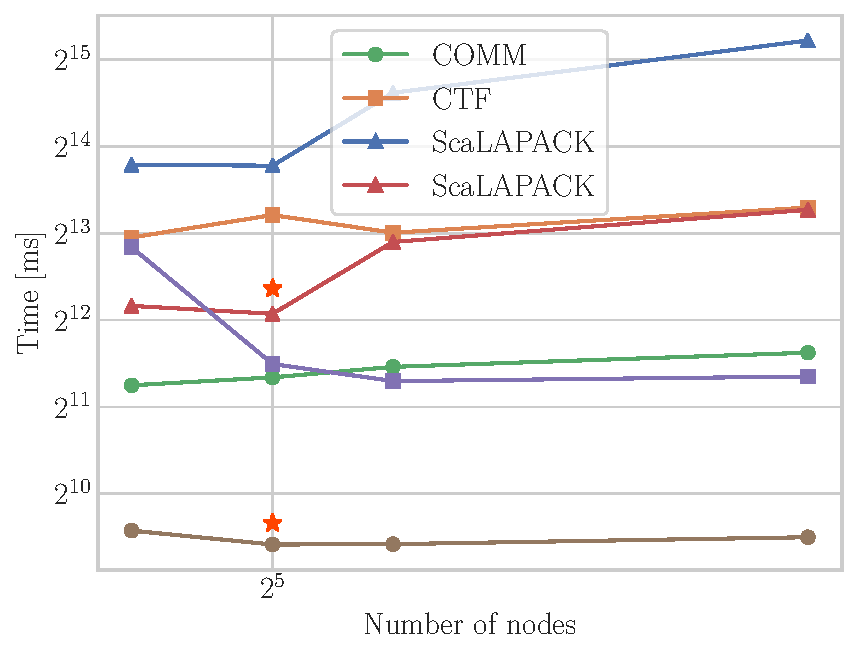
\includegraphics[width=\columnwidth]{results/thin_weak_scaling}
	\caption{"Skinny" matrices, strong scaling. $n=m=$ \greg{Missing}, $k=$ 
	\greg{Missing}} 
	\label{fig:mmmParallelization}
\end{figure}



%\begin{multline}
%\\
%G = (V,E) \\
%|V| = n \\
%|E| = m \\
%p partitions \\
%\forall_{i = 1..p} P_i \in V \\
%\bigcup_{i = 1..p} P_i = V \\
%\bigcap_{i = 1..p} P_i = \emptyset \\
%\forall_{i = 1..p} BE_i \in E = \{(u,v) : u \in P_i \land v \notin P_i\} \\
%\forall_{i = 1..p} BV_i \in V = \{u : (u,v) \in BE_i\} \\
%pl_i(u,v) = \{e \in E \cap (P_i \times P_i) : \text{edges connect u and v} \} 
%- 
%\text{local path between u and v} \\
%pr_i(u,v) = \{e \notin E \cap (P_i \times P_i) : \text{edges connect u and v} 
%\} - \text{remote path between u and v} \\
%\end{multline}
%\begin{enumerate}
%  \item For each $P_i$:
%\end{enumerate}

\section{Related work}

Works on data movement minimization essentially may be divided into two 
categories: applicable across 
memory hierarchy (vertical, also called I/O minimization), or between parallel 
processes (horizontal, also called communication minimization). Even though 
they are ``two sides of the same coin'', in literature they are often treated 
as 
separate topics. In our work we combine them: analyze
trade--offs between 
communication optimal (distributed memory) and I/O optimal schedule 
(shared memory).
% We observe that even though algorithms in the second class 
%tend to be problem size independent, distributed memory algorithms fix the 
%domain sizes based on the even process grid (as discussed in Introduction - 
%"top-down" vs "bottom-up" approach).

\subsection{General I/O Lower Bounds}
I/O optimization techniques date back to work by 
Sethi~\cite{completeRegisterProblems}, where he used a one color pebble game to 
model the minimum number of registers required to perform a computation. It has 
been proven by Gilbert et.al~\cite{pebblegameregister} that this problem is 
P-SPACE complete. Despite the complexity, much work based on the pebble game 
abstraction. Paul and Tarjan~~\cite{pebbleTradeoffs} studied the space--time 
tradeoffs in pebble games. Dymond and Tompa~\cite{dymond2playerpebblegame} 
developed a 
two-player game to study parallel speedups. Most notably, Hong and 
Kung~\cite{redblue} introduced the red-blue pebble game, on which we base our 
work. Elango et al.~\cite{redbluewhite} extended this work to the 
red-blue-white 
game and Liu and Terman~\cite{redblueHard} proved that it is also P-SPACE 
complete. Chan~\cite{justApebbleGame} studied different variants of pebble 
games in the context of memory space and parallel time. Aggarwal and 
Vitter~\cite{externalMem}
introduced a two-memory machine that models a blocked access and latency in an
external storage. Large et al.~\cite{parallelExMem} extended this model to a 
parallel machine. Solomonik et al.~\cite{edgarTradeoff} combined the 
communication, synchronization, and computation in their general cost model and 
applied 
it to several linear algebra algorithms. Our work uses a simplified model 
that does not take into account the memory block size, as in the external 
memory model, nor the cost of computation. We motivate it by assuming that the 
block size is significantly smaller than the input size, the data is layout 
contiguously in the memory, and that the computation is evenly distributed 
among processes.

\subsection{Shared Memory Optimizations}
Memory optimization for linear algebra includes such techniques as loop tiling 
and skewing~\cite{tiling}, interchanging and reversal~\cite{tiling2}. For 
programs with multiple loop nests, Kennedy and McKinley~\cite{loopFusion} 
showed various techniques for loop fusion and proved that in general this 
problem is NP-hard. Later, 
Darte~\cite{loopFusionComplexity} identified cases when this problem has 
polynomial complexity.

Toledo~\cite{IOsurvey} in his survey on Out-Of-Core (OOC) algorithms analyzed 
various I/O minimizing techniques for dense and sparse matrices, like 
multiplication, factorization, or iterative methods. 
Mohanty~\cite{MohantyThesis} in his thesis optimized various OOC algorithms for 
QR and QZ decompositions and eigenvalue computation, expressing them with MMM 
kernels. Irony et 
al.~\cite{IronyMMM} proved the I/O lower bound of classical MMM on a parallel 
machine. Ballard et al.~\cite{strassenBounds} proved analogous results for 
Strassen's algorithm. This analysis was extended by Scott et 
al.~\cite{generalStrassenBounds} to a general class of Strassen-like algorithms.

Although we consider only dense matrices, there is an extensive literature on 
sparse matrix I/O optimizations. Bender et al.~\cite{SpMVIO} extended 
Aggarwal's external memory model~\cite{externalMem} and showed I/O complexity 
of the sparse matrix-vector (SpMV) multiplication under various data layouts. 
Greiner~\cite{SpEverything} extended those results and provided parallel I/O 
complexities of other sparse computations, like bilinear forms or sparse-sparse 
and sparse-dense matrix multiplications. 

In our work we use the results from Irony et 
al.~\cite{IronyMMM} to prove the I/O optimality of COMM.


\subsection{Distributed Memory Optimizations}
Distributed algorithms for dense matrix multiplication dates back to the work 
of 
Cannon~\cite{Cannon}, which has been analyzed and extended many 
times~\cite{MManalysis}~\cite{generalCannon}. In the presence of extra memory, 
Aggarwal et al.~\cite{summa3d} included parallelization in the third dimension. 
Solomink and Demmel~\cite{25d} extended this scheme with their 2.5D 
decomposition to arbitrary range of 
the available memory, effectively interpolating between Cannon's 2D and 
Agarwal's 
3D scheme. A recursive, memory-oblivious 
MMM algorithm was introduced by 
Blumofe 
et al.~\cite{recursiveMM} and extended to rectangular matrices by Frigo et 
al.~\cite{recursiveRectangularMM}. Demmel el al.~\cite{CARMA} showed that their 
recursive CARMA algorithm achieves asymptotic complexity for all matrix and 
memory sizes. We compare COMM with these algorithms, showing that we achieve 
better results both in terms of communication complexity and the actual runtime
performance. 
Lazzaro et al.~\cite{lazzaroSpMM} used the 2.5D technique for sparse 
matrices, both for square and rectangular grids. Koanantakool et 
al.~\cite{sparse15D} observed that for sparse-dense MMM, 1.5D decomposition 
performs less communication than 2D and 2.5D schemes, as it distributes only 
the sparse matrix.

\subsection{Strassen-Like Routines}

Another class of optimizations, based on group theory,
are Strassen-like routines~\cite{Strassen}, which asymptotically reduce the
number of arithmetic operations. Currently, the algorithm with the lowest
asymptotic complexity $O(n^{2.3729}$) is by Le~Gall~\cite{LeGall}. In our work,
however, we focus only on the ``classical'' MMM algorithms which perform $n^3$
additions and multiplications, as they are often faster in practice on modern 
parallel architectures with deep memory hierarchies~\cite{strassenVsClassic}.  



\section{Conclusions}
In our work we show that starting from the sequential I/O optimality we achieve 
optimal parallel communication optimality for any combination of input 
parameters. We introduce a new proof of sequential and parallel matrix 
multiplication data movement complexity, giving tight leading constants. We 
advocate that asymptotic analysis alone is not enough to draw conclusions on 
the real-life performance of the algorithms. We 
compare (name of our algorithm here) with existing state-of-the-art schedules, 
showing the 
superiority of the former both in terms of theoretical analysis and achieved 
performance.

%\greg{
%  TODO: 
%  \begin{enumerate}
%    \item BSP model?
%  \end{enumerate}
%}
%
%\section{Bibliography}

%% Bibliography style
%\bibliographystyle{ACM-Reference-Format}

\bibliographystyle{ACM-Reference-Format}
\bibliography{mmm-ppopp}
%
%\appendix
%
%
%\section{I/O Lower Bounds for Arbitrary CDAGs}
%\label{sec:introIO}
%In this section we shortly introduce a general mathematical machinery we use 
%to 
%proof 
%the I/O optimality of COMM. We extend Lemma~\ref{lma:spartlemma} by 
%Hong and 
%Kung~\cite{redblue}, which provides a method to find an I/O lower bound for a 
%given CDAG. This lemma, however, does not give a tight bound, as it 
%overestimates a \emph{reuse set} size (cf. 
%Lemma~\ref{lma:reuse}). Our key result here, Lemma~\ref{lma:reuse} 
%allows us to derive a constructive proof of a tighter I/O lower bound for a 
%sequential execution of MMM CDAG~(\cref{sec:seqOptimality}). We use this 
%result 
%in~(\cref{sec:parOptimality}) to prove the parallel I/O optimality of COMM.
%
%Our method heavily relies on a red-blue pebble game 
%(Definition~\ref{df:redbluegame}) 
%and an $S$-partition abstractions (Definition~\ref{df:s-partition}) introduced 
%by Hong and Kung.
%
%\subsection{Red-Blue Pebble Game}
%A red-blue pebble game is an abstraction modeling an execution of an algorithm 
%in a two-level memory structure with a 
%small-and-fast
%as well as large-and-slow memory. A red (or a blue) pebble placed on a vertex 
%of a CDAG denotes that this data is inside a fast (or slow) memory.  It is a 
%powerful tool, extensible to
%arbitrarily many memory levels~\cite{redblueHierarchy}, that was used to derive
%lower bounds for algorithms such as sorting or FFT~\cite{redblue}. 
%
%\macb{Intuition}
%%
%In the red-blue pebble game, a red (or blue) pebble placed on a vertex denotes 
%that its value is inside the fast (or slow) memory.
%%
%%A computation of a 
%%CDAG starts with placing
%%certain \emph{pebbles} on its input vertices\greg{changed "certain 
%%number of pebbles" to "certain pebbles". The first one was just wrong.}, 
%%which 
%%corresponds to 
%%loading the
%%data from the slow to the fast memory. 
%%
%The actual computation (referred to as
%\emph{pebbling}) is a series of allowed moves (e.g., moving a pebble from one
%vertex to another) that correspond to load, store, compute, or
%freeing-memory operations.
%%
%The \emph{I/O cost of a computation} is the number of pebble moves that
%correspond to loads and stores between the slow and the fast memory; finding 
%the pebbling that minimizes
%this cost is PSPACE-complete~\cite{redbluecomplete, pebblegameregister}. 
%
%\begin{defn}[Red-Blue Pebble Game~\cite{redblue}] \label{df:redbluegame}
%	Let $G = (V,E)$ be a CDAG. 
%	In the initial/terminal configuration, only inputs/outputs of the CDAG have
%	blue pebbles.
%	%
%	There can be at most $S$ red pebbles used. A complete CDAG computation is a
%	sequence of moves that lead from the initial to the terminal pebble
%	configuration.
%	%
%	The allowed moves are as follows: \ding{172} placing a red pebble on any 
%	vertex
%	with a blue pebble (load), \ding{173} placing a blue pebble on any vertex 
%	with 
%	a red
%	pebble (store), \ding{174} placing a red pebble on a vertex whose parents 
%	have 
%	all red
%	pebbles (compute), \ding{175} removing any pebble (red or blue) from any 
%	vertex 
%	(freeing memory).
%\end{defn}
%
%An I/O optimal execution of a CDAG corresponds to a sequence of moves (called 
%\emph{pebbling} of a graph) which minimizes load \ding{172} and store 
%\ding{173} moves.
%
%\macb{Connections to MMM}
%%
%For a CDAG of MMM, an example pebbling moves include placing red pebbles on 
%some vertices
%corresponding to elements of matrices $A$ and $B$ (load operations), placing 
%red
%pebbles on the corresponding elements of $C$ (compute), removing red
%pebbles from the loaded inputs (freeing memory) and placing blue pebbles on the
%computed elements of $C$ (store). 
%
%\subsection{$S$-Partitions}
%
%
%The notion of an \emph{$S$-partition} facilitates deriving lower bounds on the
%I/O computation cost~\cite{redblue}. Here, one divides a given CDAG into
%consecutive \emph{subcomputations}, each of which requires at least $S$ load 
%and store
%operations. The key element in more straightforward
%lower bound proofs is to analytically bound the size (vertex count) of
%the largest subcomputation, given its input and output size (i.e., the number
%of vertices outside (inside) the subcomputation that have a child inside
%(outside) of it). 
%%
%%\macb{Intuition}
%%
%%Intuitively, the $S$-partition technique may be seen as a generalization of
%%the Loomis-Whitney inequality~\cite{loomisWhitney}, which is used in linear
%%algebra for bounding the amount of I/O~\cite{loomisApplied}: both techniques
%%aim at finding the optimal surface (communication) to volume (computation)
%%ratio in a given setting. 
%%
%%$S$-partition was used to derive the first I/O bounds for matrix
%%multiplication, FFT, or odd-even transposition sorting~\cite{redblue}.
%%
%%\macb{Details}
%%
%Formally:
%
%\begin{defn}[$S$-partition of a CDAG~\cite{redblue}] \label{df:s-partition}
%	%
%	Let $G = (V,E)$ be a CDAG. An $S$-partition of $G$ is a collection $\{V_1, 
%	...,
%	V_h\}$ of $h$ subcomputations of $ V$ such that: \ding{192} $V_i \cap V_j
%	=\emptyset\ $ and $\bigcup_{i=1}^{h} V_i=V$ for any $1 \le i,j \le h$,
%	\ding{193} $\forall i\quad |Dom(V_i)| \le S$, \ding{194} $\forall i\quad
%	|Min(V_i)| \le S$, and \ding{195} there is no cyclic dependence between
%	subcomputations.
%	%   
%	% \begin{itemize} \item $\forall_{1 \le i,j \le h}\quad V_i \cap V_j
%	% =\emptyset\ $ and $\ \bigcup_{i=1}^{h} V_i=V$ \item $\forall i\quad
%	% |Dom(V_i)| \le S$ \item $\forall i\quad |Min(V_i)| \le S$ \item there is 
%	%no
%	% cyclic dependence between subcomputations.  \end{itemize}
%	%
%\end{defn}
%
%$Dom(V_i) \not \subset V_i$ is the \emph{dominator set}: a set of vertices 
%such 
%that
%every path from an input of the CDAG to a vertex in $V_i$ contains some 
%vertex in in
%$Dom(V_i)$.
%%
%$Min(V_i) \subset V_i$ is the \emph{minimum set} of $V_i$: it contains vertices
%that do not have any children in $V_i$. 
%%
%%Throughout this paper, we will use \emph{subset} and \emph{subcomputation}
%%interchangeably, to emphasize its interpretation in the context of 
%%scheduling. 
%%
%Finally, $H(S)$ is the cardinality of the smallest valid $S$-partition of a
%given CDAG.
%
%We use a symbol $\mathcal{S}(S) = \{V_1, \dots , V_h\}$ to 
%denote an $S$-partition. 
%%
%% there is a
%%lower bound on the cardinality of a valid $S$-partition.  We denote this
%%minimal number of vertex sets with a dedicated symbol $H(S)$.
%
%\macb{Connections to MMM}
%%
%In MMM, a subcomputation $V_i$ is a calculation of partial sums of $C$ that can
%be computed with at most $S$ elements of $A$ and $B$, and that contributes to
%at most $S$ outputs. Those elements from $A$ and $B$, as well as previous
%values of $C$ being updated, form $Dom(V_i)$. Then, $Min(V_i)$ corresponds to
%the result of this subcomputation (cf.~
%Figure~\ref{fig:iterationSpace}). $H(S)$ denotes 
%the
%number of such subsets required to calculate the final result. Assuming that 
%each subcomputation computes the same number of partial results 
%$\forall_{i,j}|V_i| = |V_j|$, and observing the total number of partial 
%results 
%$|V| = mnk$, we have $H(S) = \frac{mnk}{V_i}$.
%% (geometrically
%%\mac{what does geometrically mean?}, \mac{the} number of subsets require
%%\mac{required} to fill the entire 3D iteration space \mac{what 3D space? was
%%*never* defined or even mentioned... Already complained. I think the best 
%%place
%%is the background subsection dedicated to MMM. It can be very brief (1-2 
%%sentences)}).
%
%\subsection{Existing General I/O Lower Bound}
%\label{sec:spartProof}
%
%%\greg{Observation: 2S-partition reduces scheduling problem (P-space) 
%%to 
%%partitioning problem (NP-complete)?}
%%\greg{...... UPDATE: I don't show here the proof of NP-completeness 
%%of 
%%S-partitioning. Too much space. Better skip this observation}
%
%We now cite a \emph{general} lower bound on the cost of \emph{any} I/O
%computation~\cite{redblue} and sketch the proof, which is the basis for our
%\emph{tighter general} bound on the I/O cost (Lemma~\ref{lma:reuse}).
%
%\macb{Intuition}
%%
%The key notion in the existing bound is to use $2S$-partitions for a given fast
%memory size~$S$.
%%
%For some subcomputation $V_i$, if $|Dom(V_i)| = 2S$ vertices, then at most $S$
%of them could contain a red pebble before $V_i$ begins.  Thus, at least $S$
%additional pebbles need to be loaded from the memory.  The similar argument
%goes for $Min(V_i)$. Therefore, knowing the lower bound on the number of sets
%$V_i$ in a valid \emph{$2S$-partition}, together with the observation that each
%$V_i$ performs at least $S$ I/O operations, we have:
%%
%%  a \emph{$2S$-partitioning} of the
%%graph. Thus, each subcomputation $V_i$ requires $2S$ input elements (the
%%dominator set) to perform the computation. Because at most $S$ elements could
%%already be in the fast memory from the previous computation (recall that the
%%size of the fast memory is $S$), the remaining $S$ elements have to be loaded
%%from the slow memory. 
%%
%%Similarly, because $V_i$ has $2S$ output elements (the minimum set), but only 
%%$S$
%%can be immediately consumed by the next computation, remaining $S$ elements
%%have to be stored in the slow memory. By finding the minimum number of valid
%%$S$-partition subsets \mac{why S and not 2S? This sentence seems completely
%%detached from the previous text}, we derive the I/O lower bound:
%
%\begin{lma}[Lower bound on the number of I/Os~\cite{redblue}]
%	%
%	The minimal number $Q$ of I/O operations for any valid execution of a CDAG 
%	of
%	any I/O computation is bounded by
%	
%	\begin{equation}
%	\label{eq:redbluebound}
%	Q \ge S \cdot (H(2S) - 1)
%	\end{equation}
%	%
%\end{lma}
%
%\macb{Details}
%%
%% We now sketch the original proof, as we use it as a basis for our
%% Lemma~\ref{lma:reuse}, which gives a tighter I/O bound.
%%
%Assume that we know the optimal schedule of the CDAG. Divide the computation
%into $h$ consecutive subcomputations $V_1, V_2, ..., V_h$, such that during the
%execution of $V_i$, $i < h$, there are exactly $S$ I/O operations, and in $V_h$
%there are at most $S$ operations. Now, for each $V_i$, we define two subsets of
%$V$, $V_{R,i}$ and $V_{BR,i}$.
%%
%%\begin{enumerate}[leftmargin=1.5em]
%%
%$V_{R,i}$ contains vertices that have red pebbles placed on them just before
%$V_i$ begins.
%%
%$V_{BR,i}$ contains vertices that have blue pebbles placed on them just before
%$V_i$ begins, and have red pebbles placed on them during $V_i$.
%%
%% \end{enumerate}
%%
%% \noindent
%%
%% Then, one can derive the following observations:
%%
%Using these definitions, we have: \ding{182} $V_{R,i} \cup V_{BR,i} =
%Dom(V_i)$, \ding{183} $|V_{R,i}| \le S$, \ding{184} $|V_{BR,i}| \le S$, and
%\ding{185} $|V_{R,i} \cup V_{BR,i}| \le |V_{R,i}| + |V_{BR,i}| \le 2S$.
%% 
%% \begin{enumerate}
%%   %
%%   \item $V_{R,i} \cup V_{BR,i} = Dom(V_i)$
%%   %
%%   \item $|V_{R,i}| \le S$
%%   %
%%   \item $|V_{BR,i}| \le S$
%%   %
%%   \item $|V_{R,i} \cup V_{BR,i}| \le |V_{R,i}| + |V_{BR,i}| \le 2S$
%%   %
%% \end{enumerate}
%% 
%We define similar subsets $W_{BR,i}$ and $W_{R,i}$ for the minimum set 
%$Min(V_i)$.  $W_{BR,i}$ contains all vertices in $V_i$ that have a blue 
%pebble placed on them during $V_i$, and  $W_{R,i}$ contains all vertices in 
%$V_i$ that have a red pebble at the end of $V_i$. By the definition of $V_i$, 
%$W_{BR,i} \le S$, by the constraint on the red pebbles, we have $W_{R,i} \le 
%S$, and by te definition of the minimum set,$Min(V_i) \subset W_{R,i} \cup 
%W_{BR,i}$.
%%
%Finally, by Definition~\ref{df:s-partition}, $V_1, V_2, ..., V_h$ form a valid
%$2S$-partition of the CDAG. 
%
%% We now proceed to show how we can tighten this bound by tightening the bound
%% on the set $V_{R,i}$, that is, the data reuse between the computations. 
%
%
%\subsection{Tighter General I/O Lower Bounds}
%\label{sec:seq-proof}
%
%
%\subsubsection{Data Reuse}
%\label{sec:datareuse}
%
%A more careful look at the sets $V_{R,i}, V_{BR,i}, W_{R,i}$ and $W_{RB,i}$ 
%allows us to 
%refine the bound on the number of I/O operations on a CDAG. By its 
%definition,  
%$V_{BR,i}$ is a set of vertices on which we perform move \ding{172} (load).  
%On the other hand, $V_{R,i}$ is the set of vertices that were already computed 
%(red-pebbled) during some $V_j, j < i$, and are reused during $V_i$ (the move 
%\ding{172} is not needed).  
%We call $V_{R,i}$ a \emph{reuse set} of $V_i$. Similarly, by its definition, 
%$W_{BR,i}$ contains all the vertices on which we perform move \ding{173} 
%(store)  during $V_i$.
%Therefore, if $Q_i$ is the number of I/O 
%operations during the subcomputation $V_i$, then we have $ Q_i \ge |V_{BR,i}| 
%+  |W_{BR,i}|$.
%The trivial bounds are 
%$V_{R,i} le S$ and $W_{BR,i} \ge 0$, but if one can show that $\exists_{R(S) 
%	\in \mathbb{Z}}: 
%\forall_i: V_{R,i} \le R(S) < S$ or $\exists_{T(S) \in \mathbb{Z}}: 
%\forall_i: W_{BR,i} \ge T(S)$, we can use $R(S)$ and $T(S)$ to tighten a bound 
%on 
%$Q$. We call $R(S)$ a \emph{maximum reuse} and $T(S)$ a \emph{minimum store 
%	size} of 
%a CDAG.
%
%
%\subsubsection{Reuse-based Lemma}
%
%%\greg{Just one sentence that we derive data movement optimal 
%%schedule starting 
%%from I/O optimal (sequential) schedule}
%%
%%\greg{updated}
%
%We now enhance the general I/O lower bound \emph{by tightening the bound on the
%	set $V_{R,i}$}, that is, the \emph{data reuse between the computations}
%%
%bounds. We later show the schedule attaining this bound
%(\cref{sec:seqOptimality}) and we use this schedule to minimize horizontal
%communication between processes in a distributed MMM computation
%(\cref{sec:parOptimality}). 
%%
%%\subsection{2S-partition, S-partition and data reuse}
%% \subsubsection{Tighter Sequential Bounds with Explicit Data Reuse}
%%
%% Specifically, we modify the original proof and show that finding the minimum
%% number of subsets in an $S$-partition (instead of a $2S$-partition), 
%%together 
%% with the bound on data reuse $V_{R,i}$ gives
%% tighter lower bounds.
%%
%%\macb{Intuition}
%%
%%
%Our main result in this section is as follows:
%
%\begin{lma}
%	\label{lma:reuse}
%	%
%	The minimal number $Q$ of I/O operations for any valid execution of a CDAG 
%	$\ G=(V,E)$ is bounded by  
%	
%	\vspace{-0.5em}
%	\begin{equation}
%	%
%	Q \ge (S - R(S) + T(S)) \cdot (H(S) - 1)
%	%
%	\label{eq:reusebound} \end{equation}
%	\vspace{-0.5em}
%	
%	\noindent
%	$R(S)$ is the maximum reuse and $T(S)$ is the minimum store 
%	size~(\cref{sec:datareuse}).
%	Moreover: 
%	
%	\vspace{-0.5em}
%	\begin{equation}\label{eq:reusebound-pmax}
%	H(S) \ge \frac{|V|}{|V_{max}|}
%	\end{equation}
%	\vspace{-0.5em}
%	
%	\noindent
%	where $V_{max} = \argmax_{V_i \in \mathcal{S}}|V_i|$ is 
%	the largest
%	subset of vertices in $\mathcal{S}(S)$.
%	
%	% \begin{equation}
%	% H(S) \ge \frac{|V|}{|P_{max}|}
%	% \end{equation}
%	% 
%	% Here, $S_{max} = \argmax_{S \in \mathcal{\textbf{S}}}|S|$ is an 
%	%$S$-partition
%	% of the largest size and $\mathcal{\textbf{S}}$ is a set of $S$-partitions
%	% associated with $H(S)$. \mac{double check symbols}
%	%
%\end{lma}
%
%\begin{proof}
%	%
%	To prove Eq.~(\ref{eq:reusebound}), we use analogous 
%	reasoning as in Lemma~\ref{lma:spartlemma}. We associate 
%	the optimal pebbling with $h$ consecutive subcomputations 
%	$V_1, \dots V_h$ with the difference that each 
%	subcomputation $V_i$ performs $Q_{i,s}$ store and $Q_{i,l}$ load 
%	operations, such that $S-R(S) \le Q_{i,s} \le S$ and $T(S) \le Q_{i,l} \le 
%	S$ for each $V_i$. We now define sets $V_{R,i}, V_{BR,i}, W_{R,i}$ and 
%	$W_{RB,i}$ analogously as in the previous proof. we first observe:
%	
%	\vspace{-0.5em}
%	\begin{gather}
%	\nonumber
%	\forall_{i}: (S - R(S)) \le |V_{BR,i}| \le S \\
%	\nonumber
%	\forall_{i}|V_{R,i}| \le R(S) \\
%	\nonumber
%	R(S) \le S 
%	\end{gather}
%	\vspace{-0.5em}
%	
%	Using the fact that $V_{R,i} \cup V_{BR,i} = Dom(V_i)$ 
%	(\ding{182} from~\cref{sec:spartProof}):
%	
%	\vspace{-0.5em}
%	\begin{gather}
%	\label{eq:proof}
%	\nonumber
%	|Dom(V_i)| = |V_{R,i}| + |V_{BR,i}| \\
%	\nonumber
%	|Dom(V_i)| \le R(S) + (S - R(S)) \\
%	\nonumber
%	|Dom(V_i)| \le S \\
%	\end{gather}
%	\vspace{-0.5em}
%	
%	By making analogous construction for the store 
%	operations, we show that $V_1 \dots V_h$ form a valid 
%	$S$-partition $\mathcal{S}(S)$. Therefore, a schedule 
%	performing $Q \ge (S - R(S) + T(S)) h$ operations has an 
%	associated $\mathcal{S}(S)$, such that $|\mathcal{S}(S)| 
%	= h$. By the definition $H(S) = 
%	\min_{\mathcal{S}(S)}|\mathcal{S}(S)|$, we have $Q \ge (S 
%	- R(S)) \cdot (H(S) - 1)$.
%	
%	%	$|V_{BR,i}|$ is the amount of data loaded by 
%	%subcomputation~$V_i$, lower 
%	%	bounded as stated in Eq.~(\ref{eq:proof}). Now, if each
%	%	subcomputation in a valid $S$-partition performs at least 
%	%$S - R(S)$ I/O
%	%	operations and $H(S)$ is the lower bound on their number, 
%	%then $Q \ge (S -
%	%	R(S)) \cdot (H(S) - 1)$.
%	
%	To prove Eq.~(\ref{eq:reusebound-pmax}), observe that $V_{max}$ by 
%	definition
%	is the largest subset in the optimal $S$-partition. As the subsets are
%	disjoint, any other subset covers fewer remaining vertices to be pebbled 
%	than
%	$P_{max}$. Because there are no cyclic dependencies between subsets, we can
%	order them topologically as $V_1, V_2, ...V_{H(S)}$. To ensure correct 
%	indices,
%	we also define $V_0 \equiv \emptyset$. Now, define $W_i$ to be the set
%	of vertices not included in any subset from $1$ to $i$, that is $W_i = V -
%	\bigcup_{j=1}^{i} V_j$. Clearly, $W_0 = V$ and $W_{H(S)} = \emptyset$. 
%	Then, we
%	have
%	
%	\vspace{-0.5em}
%	\begin{alignat}{2}
%	%
%	\nonumber
%	\forall_{i}\quad |V_i| & \le |V_{max}| \\
%	\nonumber
%	|W_i| = |W_{i-1}| - |V_i| & \ge |W_{i-1}| - |V_{max}| \ge i|V_{max}| \\
%	\nonumber
%	|W_{H(S)}| = 0 & \ge H(S) \cdot |V_{max}| 
%	%
%	\end{alignat}
%	\vspace{-0.5em}
%	%
%	that is, after $H(S)$ steps, we have $H(S) |V_{max}| \ge |V|$.
%\end{proof}
%
%%\subsection{I/O Bounds and Computational Intensity}
%%\label{sec:compIntensity}
%
%
%\subsubsection{Computational Intensity}
%\label{sec:compIntensity}
%
%For graphs of parametric sizes (e.g., MMM graph has $mnk + mk + kn$ vertices), 
%we need a tool to allow us to bound the I/O complexity of the whole graph by 
%bounding the maximum size of a single subcomputation. We provide an 
%observation 
%that connects the minimal 
%number $Q$ of
%I/O operations
%(cf.~Eq.~(\ref{eq:reusebound})) and a notion
%of \emph{computational intensity}.
%%
%Define computational intensity of the subcomputation $V_i$ as $\rho_i =
%\frac{|V_i|}{V_{BR,i} + W_{BR,i}}$. Intuitively, computational intensity is 
%the 
%ratio of 
%the number of computed elements ($|V_i|$) and the number of loaded and stored 
%vertices ($V_{BR,i} + W_{BR,i}$). Having the bounds $S - R(S)$ and $T(S)$ on 
%$V_{BR,i}$ and $W_{BR,i}$, respectively, and inserting Inequality 
%\ref{eq:reusebound-pmax} to \ref{eq:reusebound}, we 
%derive the following corollary:
%
%\begin{corollary*}[Computational intensity]
%	\label{cor:q}
%	Denote $\rho = \max_i(\rho_i) \le \Big(\frac{|V_{max}|}{S-R(S) + 
%		T(S)}\Big)$. Then, the number of I/O operations $Q$ is bounded by:
%	\begin{equation}
%	Q \ge \frac{|V|}{\rho}
%	\end{equation} 
%\end{corollary*}
%
%\subsubsection{$2S$-Partition vs $S$-Partition: An MMM Example}
%
%\label{sec:mmmExample}
%
%% \begin{figure}
%%  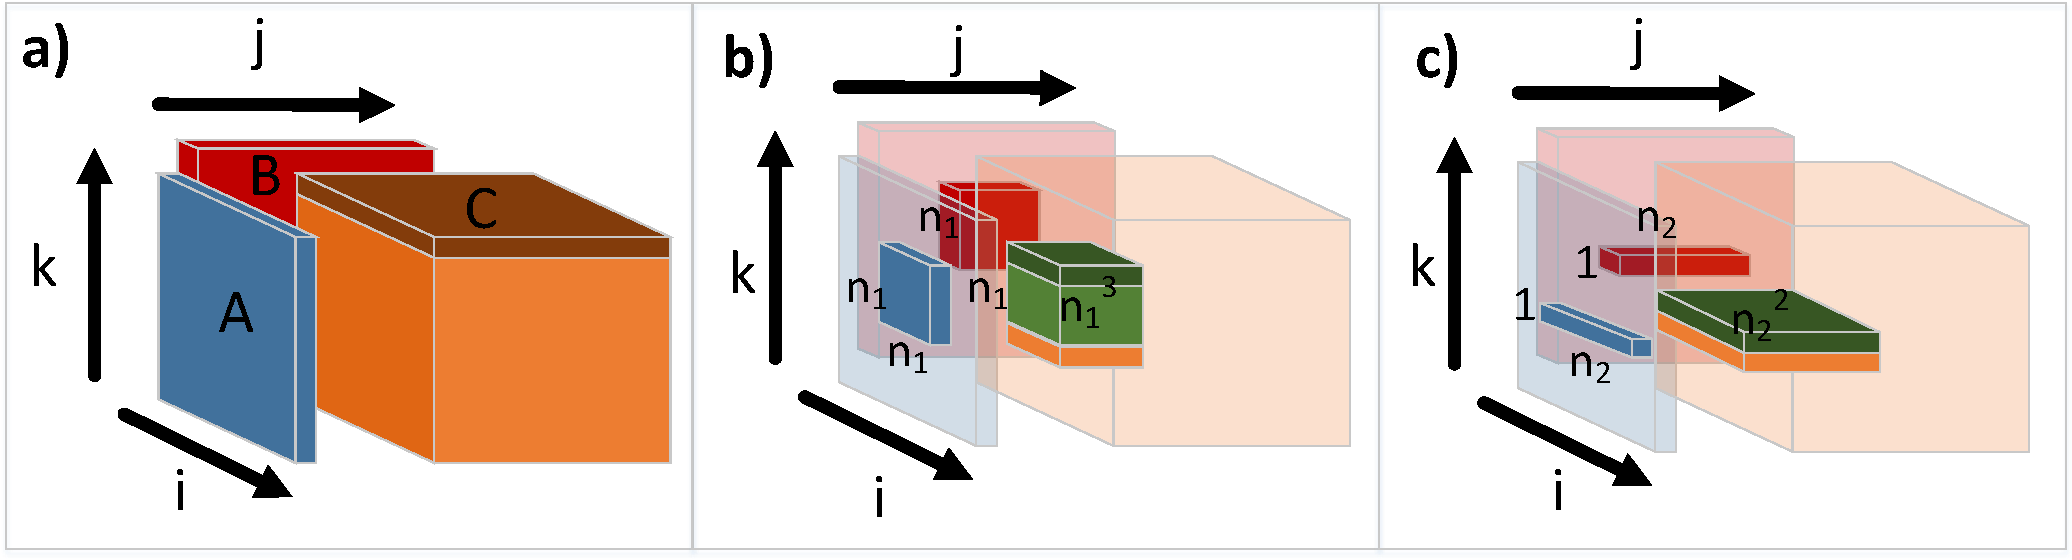
\includegraphics[width=\columnwidth]{figures/mmm_reuse}
%%  \caption{MMM subset shape. a) 
%%    geometric interpretation of $C = A B$ (orange cube represents 
%%    3-dimensional iteration space of partial sums, matrix C is formed by 
%%    reduction over dimension $k$ - represented by dark orange plane). b) 
%%    optimal surface to volume subset shape. Note that in a subsequent 
%%    subset computation only one of the three planes (blue, red or dark 
%%    green) can be reused. c) the optimal subset shapes when 
%%    data reuse is considered. In b) and c) blue, red, and orange surfaces 
%%    form the dominator set, whereas dark green surface is the 
%%    minimum set.}
%%  \label{fig:mmmreuse}
%%\end{figure}
%
%To show why Lemma 2 gives a tighter bound than Lemma 1, consider a CDAG of 
%MMM.  We can draw it in a 3D iteration space $\mathcal{V}$.
%(\cref{sec:iterationSpace}, ~\ref{fig:iterationSpace}). Then,
%an $S$-partition is a decomposition of this space into subcomputations $V_i$ 
%whose
%number of inputs ($|\alpha_i| + |\beta_i| + |\gamma_i|$) is smaller than $S$.
%When a subcomputation is viewed as a subspace in the iteration space $V_i \in 
%\mathcal{V}$, this input constraint may be viewed as a generalization of the 
%Loomis-Whitney inequality~\cite{loomisWhitney}, which relates a cardinality of 
%a 
%finite set in $\mathbb{Z}^t$ with cardinalities of its projections to all $t$ 
%dimensions. This technique was used by Irony et al.~\cite{loomisApplied} to 
%derive first parallel I/O MMM lower bounds.
%
%Assume that each subcomputation forms a cuboid $[a \times b \times c]$ in this
%iteration space (we actually prove it in~\cref{sec:seqScheduling}). Its
%faces form the dominator set.  Now based on Lemma~\ref{eq:redbluebound}, we 
%construct a $2S$-partition with a
%minimal cardinality, deriving subcomputations of a cubic ($a = b = c$) shape
%(Figure~\ref{fig:iterationSpace} b), with a cube side $a = \sqrt{2S/3}$.  Such
%schedule will perform $2a^2 \frac{n^3}{a^3} =
%\sqrt{\frac{3}{2}}\frac{2N^3}{\sqrt{S}}$ I/O operations. 
%
%Now, the question is: what is the size of a maximum reuse $R(S)$? Observe that
%only one of three faces of this cuboid can be reused (used by a subsequent
%subcomputation while still being in fast memory). This observation will help us
%derive in (~\cref{sec:seqScheduling}) a "flat" shape (Figure 
%\ref{fig:iterationSpace}
%c) which performs $\frac{2N^3}{\sqrt{S}}$ I/O operations - an $\sqrt{3/2}$
%improvement.
%
%
%\section{\hspace{-0.5em}Optimal Sequential Matrix Multiplication}
%\label{sec:seqOptimality}
%
%We now proceed to establish a tight sequential I/O lower bound of MMM. Using 
%the 
%mathematical machinery of 
%Lemma~\ref{lma:reuse}, we show a constructive proof of $Q \ge 2MNK/\sqrt{S} + 
%MN$. This result has three main contributions (1) it is an additive 
%improvement 
%over the bound $2mnk/\sqrt{S} - 2S$ by Smith and van de Geijn~\cite{tightMMM} 
%by an
%additive factor of $2S + mn$, (2) the proof is constructive - what immediately 
%follows is a corresponding schedule, (3) generality of a used technique is 
%later used to derive I/O optimal parallel schedule~(\cref{sec:parOptimality}) 
%and may be used in other 
%linear algebra problems.
%%
%%\mac{the} I/O lower bound of MMM \mac{Now I'm confused, is it the
%%new proof that is a new contribution, or the lower bound, or both? If the
%%proof, then WHY does it matter that you have a new proof? What's the deep
%%insight coming from this proof? And then why do you comment on tightening the
%%bound (below), if it's just a proof? And if it's the bound that is the new
%%contribution, then say it (underline it better!) and remove the ``new'' proof
%%adjective. And if it's both, then just make this sound better here} \mac{add
%%here ``, namely''} $Q \ge \frac{mnk}{\sqrt{S}} + mn$ \mac{,} and show a
%%schedule achieving it. This result will be used in
%%Section~\cref{sec:parOptimality} to prove tight bounds for parallel execution
%%and a schedule that is \emph{independent of any combination of problem
%%parameters} \mac{I would make this sentence the last in this paragraph}.
%%%
%%We derive \emph{all} constant terms improving the well-known asymptotic 
%%results
%%due to Hong and Kung~\cite{redblue} and Irony et al.~\cite{IronyMMM}, and
%%tightening the bound $2mnk/\sqrt{S} - 2S$ by Smith and van de Geijn by an
%%additive factor of $2S + mn$ \mac{I think it's better to place this sentence
%%right after the sentence with the lower bound, to immediately justify why this
%%new result matters}.
%%
%%\mac{Just in case, old beginning is below, commented}
%%%   
%%%   We now proceed to establish a key step to our main result. Using the 
%%%   mathematical machinery of Lemma 2, we show a new proof of I/O lower bound 
%%%of 
%%%   MMM $Q \ge \frac{mnk}{\sqrt{S}} + mn$ and show a schedule achieving it. 
%%%This 
%%%   result will be used in Section~\cref{sec:parOptimality} to prove tight 
%%%bounds 
%%%   for parallel execution and a schedule 
%%%   that is \emph{independent of any combination of problem parameters}.
%%%   %
%%%   We derive \emph{all} constant terms improving the well-known asymptotic
%%%   results due to Hong and Kung~\cite{redblue} and Irony et 
%%%al.~\cite{IronyMMM}, 
%%%   and tightening the bound $2mnk/\sqrt{S} - 2S$ by Smith and van de Geijn by
%%%   an additive factor of $2S + mn$.
%%
%%
%%\greg{commented out the whole subsection Top-down vs bottom-up. It is 
%%mentioned 
%%in the intro and not needed here at all.}
%
%%\subsection{Top-Down vs Bottom-Up}
%%
%%\mac{The title is a bit confusing... Maybe we can remove it completely}
%%
%%\mac{No, I would start differently - with stating our approach, underlying 
%%what
%%is the paper contribution! E.g., "We do bottom-top (see Figure X), as opposed 
%%to [all
%%others], [here is briefly why]}
%%%
%%Most of the current state-of-the-art algorithms, like Cannon's~\cite{Cannon},
%%SUMMA~\cite{summa}, 3D SUMMA~\cite{summa3d}, or the 2.5D scheme~\cite{25d}
%%use the "top-down" approach, that is, aim for decomposing the global domain
%%evenly into $p$ processes (Figure \ref{fig:topdown-vs-bottomup}).
%%%
%%To obtain our schedule and prove its optimality, we use "bottom-up" approach,
%%that is, defining the finest-granularity task for a single process and then
%%identifying parallelization opportunities.  
%%%
%%\mac{Man, why do you provide this whole following part on task based
%%programming?  What connection does it have? I would remove it completely, or
%%move to a place where task based stuff is used...} 
%%%
%%Intuitively, the "bottom-up" approach shares similarities with task-based
%%programming~\cite{taskparalelism}, which has also be used in the context of
%%linear algebra~\cite{taskMMM}. The difference, however, is in the
%%\emph{granularity}: A task is a single, I/O optimal, rank-1 \mac{rank-1 was 
%%not
%%defined} update (vector-vector outer product), instead of coarser grained
%%rank-k \mac{rank-k was not defined} updates (matrix-matrix product) in
%%recursive algorithms, like CARMA~\cite{CARMA}.
%%%
%
%%
%%\subsection{Tight MMM Lower Bound}
%%\label{sec:seqScheduling}
%%
%%
%%\greg{commented out the whole beginning}
%%\mac{Bad, you should provide some beginning in this paragraph}
%
%%
%%\mac{This title is too long}
%%
%%\mac{The following sequence is broken - how can algorithms
%%derive their proofs? Moreover, ``derives'' should be ``derive'', right?}
%%%
%%"Top-down" algorithms, discussed in Section \ref{sec:seqOptimality}, 
%%derives
%%their 
%%optimality proofs from maximizing computation to communication (input volume) 
%%ratio.
%%%
%%\mac{At this point, I again think that it's bad because you start with 
%%describing
%%others, and not the stuff in this paper}
%%The key difference between them, as well as the original lower bound lemma 
%%(inequality 
%%\ref{eq:redbluebound}) and the lemma presented in this paper (inequality 
%%\ref{eq:reusebound}) is the explicit notion of reuse. \mac{The following 
%%sentence
%%sounds like a reasonable first sentence in this section...} In this section, 
%%we prove 
%%optimal sequential scheduling, \mac{The following sentence part is broken?} 
%%which later be used to derive parallelization 
%%strategies.
%%%
%%\mac{Why do I care? Underline ``what'' parallelization strategies you will
%%obtain - optimal? near-optimal? faster than others? Make this announcement 
%%(parallelization strategies)
%%sounds more interesting... Also, strategies of what?} 
%%%
%%The crucial insight is that it is independent of matrix dimensions 
%%and machine model (distributed or shared memory).
%%%
%%\mac{What? At this point I'm confused. You always wrote about this stuff 
%%being 
%%independent of
%%problem parameters. But saying it's independent of machine model is extremely 
%%confusing,
%%considering the fact that you devoted so much space to describing I/O, etc 
%%etc...}
%%%
%%\mac{In addition: ``it is independent of matrix dimensions
%%and machine model'' is *not* a crucial insight... this is the advantage of
%%this scheme. Insight is sth deep, some observation about the nature of 
%%something.}
%%%
%%\mac{The following sentence: this is not a place for this... You should 
%%discuss such
%%things in related work. Sure, sometimes, one must discuss such connections 
%%before
%%related work, but make it concrete and to the point. Right now, you just say 
%%`` We do X differently than others''. Why do I care? How does it help me 
%%understand
%%this section better?}
%%%
%%We use different technique than used by Smith and van de Geijn, who proved 
%%sequential lower bound $2mnk/\sqrt{S} - 2S$ and prove a lower bound tighter 
%%\mac{TIghter?
%%Then why are we still better?} by 
%%a constant factor of $2S$ :  $2mnk/\sqrt{S}$. Furthermore, the former result 
%%does not count storing the output, which yields additional $mn$ I/O 
%%operations.
%%\mac{Again, at this point I read 15 lines of text in this *core* and *key* 
%%section
%%that should focus on describing your idea, and still I have no idea... more 
%%than 30\%
%%of this paragraph are some general notes, without obvious connection to the 
%%flow of
%%*this* section, about others' work. How should it help the reader understand 
%%this
%%section better?}
%%
%%\mac{The whole following part is again out of the place... I mean, shouldn't 
%%it be
%%explained in Background? How does it relate to the models from Background?}
%%We use the computation model from Hong and Kung~\cite{redblue}, that is:
%%\begin{enumerate}
%%  \item A machine has a fast memory of size $S$ and a slow memory of infinite 
%%  size,
%%  \item all computations have to be performed inside fast memory, \mac{Huh?
%%  But this sounds like you completely prevent *any* I/O during the execution?
%%  So what's the point of I/O complexity anyway?}
%%  \item at the beginning of computation, all inputs are in slow memory, and 
%%  at the end of computation all the outputs must be stored back to slow 
%%  memory. 
%%\end{enumerate}
%%
%
%\begin{thm}[Sequential Matrix Multiplication I/O lower bound] 
%	%Multiplying matrices of sizes $m \times k$ and $k \times m $ in the 
%	%computation 
%	%model from Definition~\ref{df:redbluegame} requires a minimum number of 
%	%I/O 
%	%operations is $\frac{mnk}{\sqrt{S}} + mn$.
%	Multiplying matrices of sizes $m \times k$ and $k \times m $ requires a 
%	minimum 
%	number of $\frac{mnk}{\sqrt{S}} + mn$ I/O operations.
%	\label{thm:seqlowbounds}
%\end{thm}
%
%\begin{proof}
%	
%	We first discuss a short intuition behind
%	the proof. Next, we provide all details.
%	
%	\macb{Proof Intuition}
%	%
%	Using Lemma~\ref{lma:reuse}, we first establish a valid subset $V_i$ of an
%	$S$-partition that achieves maximum computational intensity $\rho$ and find 
%	its
%	size (the number of vertices). Knowing $\rho$ and that there are $mnk$
%	vertices in the whole MMM CDAG, we find the total
%	I/O cost of the complete execution. Throughout the proof, in addition to
%	full details, we include intuitive interpretations of key steps. To
%	help keep up with the intuition, assume that $V_i$ is a 
%	cuboid~(\cref{sec:iterationSpace}), and that we want to find its optimal 
%	size 
%	under certain conditions.
%	
%	%\greg{your comments are commented out}
%	%  
%	%\mac{It may be a good idea to first have a titled paragraph like here, with
%	%the outline of the proof, followed by the (titled again) rest.}
%	%%
%	%We first derive a size \mac{Did you define precisely ``size of an 
%	%S-partition?}
%	%and shape \mac{``shape of an S-partition'' was clearly not defined before} 
%	%of
%	%an elementary \mac{What is ``elementary'' in this context? Again a 
%	%confusing
%	%word} S-partition subcomputation (subset) \mac{It seems these two words
%	%(subcomputation, subset) mean the same thing? Use only one
%	%consistently} $P$ that achieves 
%	%maximum computational intensity $\rho$ \mac{I would explain briefly WHY 
%	%you 
%	%need
%	%to derive this particular S-partition}. We then show the 
%	%number of I/O operations per $P$ and derive the number of $P$ required to 
%	%perform the whole computation. \mac{Again, I would briefly describe
%	%the general intuition of the whole proof and the most important steps}
%	
%	\macb{Full Proof}
%	%
%	In this proof, we will use the iteration space 
%	$\mathcal{V}$~(\cref{sec:iterationSpace}) to represent the 
%	CDAG of MMM.
%	By Definition~\ref{df:s-partition}, we divide the whole computation into
%	$H(S)$ subcomputations $V_i, i \in \{1,\dots H(S)\}$, such that $Dom(V_i), 
%	Min(V_i) \le 
%	S$. As stated in~(\cref{sec:iterationSpace}), the dominator set of 
%	$V_i$ is $Dom(V_i) =\phi_{ik}(V_i) \cup \phi_{kj}(V_i) \cup \phi_{ij}(V_i) 
%	= 
%	\alpha_i \cup \beta_i \cup \gamma_i$. Because all the read-after-write 
%	(RAW) 
%	dependencies are parallel to the vector~\textbf{k} (Line 5 in 
%	Listing~1), the projection of the minimum set $Min(V_i)$ onto the plane 
%	\textbf{ij} is also equal to $\gamma_i$ : ($\phi_{ij}(Min(V_i)) = 
%	\gamma_i$).
%	
%	\textbf{Intuition:}  $\alpha_i, \beta_i$ and
%	$\gamma_i$ are the faces of our cuboid $V_i$. The ``bottom'' face $\gamma_i$
%	(Figure~\ref{fig:iterationSpace}) is formed by partial results of $C$ from
%	previous subcomputations, and the ``top'' face is formed by partial results
%	evaluated by $V_i$, also forming input for
%	the next subcomputation. Because all the dependencies are facing 
%	``upwards'', 
%	the minimum set (the ``top'' face) is positioned directly above the 
%	required 
%	partial results of $C$, that is $\phi_{ij}(Dom(V_i)) = \phi_{ij}(Min(V_i))$.
%	
%	By the definition of $S$-partition, we have:
%	
%	\begin{gather}
%	\label{eq:dm}
%	|Dom(V_i)| = |\alpha_i| + |\beta_i| + |\gamma_i| \le S \\
%	\nonumber
%	|Min(V_i)| = |\gamma_i| \le S
%	\end{gather}
%	
%	
%	
%	On the other hand, the Loomis-Whitney
%	inequality~\cite{loomisWhitney} bounds the volume of $V_i$: 
%	
%	\begin{equation}
%	\label{eq:lm}
%	V_i \le \sqrt{|\alpha_i| |\beta_i| |\gamma_i|}
%	\end{equation}
%	
%	
%	%\textbf{Intuition:} Loomis-Whitney inequality bounds the volume of our 
%	%cuboid
%	%by the size of its faces.  \mac{I miss here some short text stating this
%	%inequality and explaining how/why (formally) you can actually use it in our
%	%context}
%	
%	Now we proceed to find the upper bound on the maximum reuse size $R(S) = 
%	\max_{j = 1 \dots
%		H(S)}(|V_{R,i}|)$. Consider two subsequent computations, $V_i$ and 
%		$V_{i+1}$.
%	Right after $V_i$, $\alpha_i$, $\beta_i$ and $\gamma_i$ may have red 
%	pebbles on 
%	them (they are in the fast memory). On the other hand the dominator set of 
%	$V_{i+1}$ is $Dom(V_{i+1}) = \alpha_{i+1} \sum \beta_{i+1} \sum 
%	\gamma_{i+1}$.
%	Then, the reuse set $V_{R,i+1}$ is an intersection of those two sets:
%	
%	\begin{gather}
%	\nonumber
%	V_{R,i+1}
%	\subset (\alpha_i \cup \beta_i \cup \gamma_i) \cap (\alpha_{i+1} 
%	\cup 
%	\beta_{i+1} \cup \gamma_{i+1}) \\
%	\label{eq:vri1}
%	= (\alpha_i \cap \alpha_{i+1}) \cup ( 
%	\beta_i \cap 
%	\beta_{i+1}) \cup (\gamma_i \cap \gamma_{i+1})
%	\end{gather}
%	
%	\textbf{Intuition:}
%	Visualizing $V_i$ and $V_{i+1}$ as two cuboids, they can only be positioned 
%	in 
%	the 3D space so that 
%	they share at most one of their sides (either $\alpha_i \cap \alpha_{i+1} 
%	\ne 
%	\emptyset$ or  $\beta_i \cap \beta_{i+1} \ne \emptyset$ or  $\gamma_i \cap 
%	\gamma_{i+1} \ne \emptyset$ ). If we allow other shapes than cuboids, 
%	their shared surface is a sum of its projections into the three planes,  
%	$\alpha_i \cap \alpha_{i+1}$,   $\beta_i \cap \beta_{i+1}$, and $\gamma_i 
%	\cap 
%	\gamma_{i+1}$.
%	
%	
%	Note that $\alpha_i, \beta_i \subset \mathcal{I}$ are inputs of the 
%	computation:
%	therefore,
%	by the Definition~\ref{df:redbluegame}, they start in the slow memory (they 
%	already have blue 
%	pebbles).
%	$\gamma_i$, on the other hand, is the projection of the
%	minimum set $\phi_{ij}(Min(V_i)) = \gamma_i$. Therefore, at the end of 
%	$V_i$, 
%	vertices in $Min(V_i)$ may have only red pebbles
%	placed on them (they may have not been stored back to the slow memory yet). 
%	Furthermore, by the Definition~\ref{df:s-partition}, these 
%	vertices have children that have not been pebbled yet. 
%	They either have to be reused forming the reuse set $V_{R,i+1}$, or
%	stored back, forming $W_{BR,i}$ and requiring the placement of the blue 
%	pebbles. 
%	Because by their definition, $\gamma_i \cap \alpha_i = \gamma_i \cap 
%	\beta_i = 
%	\emptyset$, we have $\gamma_i \cap V_{R,i+1} =  \gamma_i \cap
%	\gamma_{i+1}$ and $W_{BR,i} =  \gamma_i \setminus
%	\gamma_{i+1}$. Then, the number of I/O operations $Q_i$ performed by the 
%	subcomputation $V_i$ (cf. Lemma~\ref{lma:reuse}):
%	
%	\begin{equation}
%	\label{eq:qi}
%	Q_i \ge |Dom(V_i)| - |V_{R,i}| + |W_{BR,i}|
%	\end{equation} 
%	
%	\textbf{Intuition:} The dominator set of each subcomputation consists of 
%	certain
%	elements from input matrices $A$ and $B$, as well as the partial results
%	of $C$. The number of loads
%	required by $V_i$ is the size of the dominator set $Dom(V_i)$ reduced by the
%	elements already loaded (the reuse set $V_{R,i}$). The number of stores is 
%	equal to the
%	number of outputs $|\gamma_i|$  that are not reused in subcomputation 
%	$V_{i+1}$, that is, 
%	not contained in $|\gamma_{i+1}|$.
%	
%	We now proceed to find $\alpha_i, \beta_i$, and $\gamma_i$
%	that maximizes the computational
%	intensity $\rho_i = \rho$ (~\cref{sec:compIntensity}).
%	We can bound $\rho_i$ by inserting Equations~\ref{eq:dm}, \ref{eq:lm}, 
%	~\ref{eq:vri1} and~\ref{eq:qi}:
%	
%	\begin{gather}
%	\nonumber
%	\rho_i = \frac{|V_i|}{|Dom(V_i)| - |V_{R,i}| + |W_{BR,i}|} \\
%	\nonumber
%	\le 
%	\frac{\sqrt{|\alpha_i||\beta_i||\gamma_i|}}{|\alpha_i| + |\beta_i| + 
%		|\gamma_i| - |\gamma_i \cap \gamma_{i+1}| +  |\gamma_i \setminus 
%		\gamma_{i+1}|}
%	\end{gather}
%	
%	We immediately see that to maximize $\rho_i$, we have $\gamma_{i+1} = 
%	\gamma_i$, as it both maximizes $|\gamma_i \cap 
%	\gamma_{i+1}|$ and minimizes $|\gamma_i \setminus \gamma_{i+1}|$.
%	
%	We then formulate it as an 
%	optimization problem:
%	
%	%Inserting Equation~\ref{eq:vri1} to~\ref{eq:qi} we see that to minimize 
%	%$Q_i$ 
%	%we have $\gamma_{i+1} = \gamma_i$, as it both maximizes $|\gamma_i \cap 
%	%\gamma_{i+1}|$ and minimizes $|\gamma_i \setminus \gamma_{i+1}|$, while 
%	%$|Dom(V_i)|$ does not depend on the choice of $\gamma_{i+1}$.
%	%
%	%
%	%W.l.o.g., assume that the subcomputation $V_i$ 
%	%achieves the maximum computational
%	%intensity $\rho_i = \rho$ (~\cref{sec:compIntensity}). To
%	%find $\alpha_i, \beta_i$ and $\gamma_i$, we formulate it as the 
%	%optimization 
%	%problem:
%	
%	
%	
%	%\begin{multline}
%	%\\
%	%\text{maximize } \rho = \frac{|V_i|}{|Dom(V_i)| - |V_{R,i}| + |W_{BR,i}|} 
%	%\\
%	%\text{subject to: } |Dom(V_i)| \le S \\
%	%\end{multline}
%	
%	\begin{multline}
%	\\
%	\text{maximize }
%	\sqrt{\gamma_i}\frac{\sqrt{|\alpha_i| |\beta_i|}}{|\alpha_i| + |\beta_i|}\\
%	\text{subject to: } \\
%	|Dom(V_i)| = |\alpha_i| + |\beta_i| + |\gamma_i| \le S \\
%	|\alpha_i|, |\beta_i|, |\gamma_i| \in \mathcal{Z} 
%	\end{multline}
%	
%	Observe that to maximize $\frac{\sqrt{|\alpha_i| |\beta_i|}}{|\alpha_i| +
%		|\beta_i|}$ we have $|\alpha_i| = |\beta_i|$. Then the solution to this
%	maximization problem gives  $|\alpha_i| = |\beta_i| \rightarrow 0$, 
%	$|\gamma_i|
%	\rightarrow S$. But because $\alpha_i$, $\beta_i$ and $\gamma_i$ are sets 
%	of 
%	vertices, therefore $|\alpha_i|, |\beta_i|, |\gamma_i| \in \mathcal{Z}$.
%	Furthermore, we have $\phi_{kj}(\alpha_i) =
%	\phi_{ik}(\beta_i)$, $\phi_{ij}(\alpha_i) = \phi_{ik}(\gamma_i)$ and
%	$\phi_{ij}(\beta) = \phi_{kj}(\gamma)$. Finally, we get:
%	
%	\begin{multline}
%	\label{eq:seqSolution}
%	\\
%	|\alpha_i| = |\beta_i|= \left \lfloor{\sqrt{S + 1} - 1} \right \rfloor \\
%	|\phi_{kj}(\alpha)| = |\phi_{ik}(\beta)| = 1 \\
%	|\gamma| = |\alpha| |\beta| = \left \lfloor{(\sqrt{S + 1} - 1)^2} \right 
%	\rfloor 
%	\\
%	\end{multline}
%	
%	
%	
%	From now on, to keep the calculations simpler, we use the following 
%	approximation:
%	
%	\begin{equation}
%	\label{eq:approx}
%	\left \lfloor{\sqrt{S + 1} - 1} \right \rfloor \approx \sqrt{S}
%	\end{equation}
%	
%	All the following results may be easily rewritten using the precise formula 
%	and
%	are correct up to this approximation factor.
%	
%	Using the approximation~\ref{eq:approx}, we have $|V_i| = S, R(S) = V_{R,i} 
%	= 
%	|\gamma_i| = S, \rho =
%	\sqrt{S}/2$.
%	Finally,  by Corollary \ref{cor:q}:  
%	$$Q \ge
%	\frac{|V|}{\rho} = \frac{2mnk}{\sqrt{S}}$$ 
%	This is the I/O cost of putting a red pebble at least once on every vertex 
%	in 
%	$\mathcal{V}$. Note however, that we did not put any
%	blue pebbles on the outputs yet (all vertices in $\mathcal{V}$ had only red
%	pebbles placed on them during the execution). By
%	Definition~\ref{df:redbluegame}, we need to place blue pebbles on $mn$ 
%	output
%	vertices, corresponding to the output matrix $C$, resulting in additional 
%	$mn$
%	I/O operations, yielding final bound
%	$$Q \ge \frac{2mnk}{\sqrt{S}} + mn$$ 
%	%
%\end{proof}
%
%\subsection{I/O Optimal Schedule}
%\label{sec:seqScheduling2}
%
%The proof of Theorem~\ref{thm:seqlowbounds} is constructive:
%that is, from it we immediately obtain a schedule achieving it. The optimal
%subcomputation $V_i$ corresponds to $S$ calculated partial products of C. Its
%inputs $\alpha$ and $\beta$ are subsets of a single column of $A$ and a single
%row of $B$, both of length $\sqrt{S}$. This may be viewed as an outer product
%formulation of MMM: each subcomputation is an outer product of two vectors of
%length $\sqrt{S}$, with subsequent subcomputations updating this result
%(Listing~\ref{lst:pseudocode}).
%
%\begin{lstlisting}[float=h, caption=Pseudocode of I/O optimal sequential MMM, 
%label=lst:pseudocode]
%T = $\sqrt{S}$
%for i_1 = 1:m/T
%	for j_1 = 1:n/T
%		for r = 1:k    % k is the outer loop
%			%elementary subcomputation V
%			for i_2 = i_1*T : (i_1+1)*T
%				for j_2 = j_1*T : (j_1+1)*T
%					C(i_2,j_2) = C(i_2,j_2) + A(i_2,r)*B(r,j_2)
%				end for
%			end for 
%		end for
%	end for 
%end for
%\end{lstlisting}
%%
%%We note that an implementation based on this outer
%%schedule is the Goto algorithm~\cite{Goto}. 
%
%%-------------old version starts here----------%
%%\greg{------------old version starts here -----------} 
%%
%%
%%
%%Let's \mac{Let's is too informal} represent the matrix multiplication 
%%operations \mac{What are ``matrix multiplication operations''?
%%again, confusing. Intuitively it may be clear, but this must be precise. The 
%%actual products of matrix elements? the sums? more precision} as the three 
%%dimensional 
%%iteration space \mac{This is much more your domain and not main, but 
%%``iteration space'' also
%%sounds quite vague}. Let $i,j,k$ be dimensions corresponding to matrix sizes 
%%$m,n,k$, that is, matrix $A$ lays on the plane $ik$, matrix $B$ lays on the 
%%plane $kj$ and matrix $C$ lays on the plane $ij$ \mac{This again is somewhat 
%%confusing. What is ``plane'' mathematically here?
%%This is proof, all must be clear. Define plane... But then I know, there are 
%%many
%%of these concepts (as we discussed while hiking), and defining them all
%%would be very tedious... My recommendation - \ul{I suggest you read several
%%proofs from top math conferences related to this type of things, and see how 
%%people deal with this}}.
%%
%%\mac{\ul{Another important comment:} at this point, it becomes clear that
%%the paper lacks some background into the MM stuff. I mean, you need to
%%lay out the setting... All these MM-related concepts such as laying matrices
%%A, B, C onto different ``planes of computation'' must be introduced in
%%Background.}
%%%
%%Assume that the searched subset \mac{I would use some symbol for this subset
%%that maximizes intensity} computes $\mathcal{V}$ partial products $c = c + ab$
%%\mac{what? why $c = c + ab$? Mathematically, unless $ab=0$, it's never true,
%%right?} of $C$ \mac{\ul{First comment:} Also, it's confusing: what are
%%``products of $C$''??}. Then, the projection of $\phi_{ik}(\mathcal{V})$
%%\mac{``Projection'' was never defined (extremely confusing). \ul{Second
%%comment:} Moreover: what is this $\mathcal{V}$? it is also not defined. In the
%%sentence before, it sounds like a number (``$\mathcal{V}$ products''), but 
%%here
%%it sounds more like something more complex than a number? Again confusing.
%%\ul{Third comment}: is it "the projection of" OR "the projection"? It makes a
%%huge difference. Now it sounds like it should be "the projection" (and is
%%wrongly "the projection of"} onto plane $ik$ correspond \mac{``corresponds''
%%instead of ``correspond''?} to the required inputs from $A$.  \mac{Very
%%confusing - WHY does this projection correspond to the input? It will be
%%unclear to the reader... Maybe with the proper background it will clarify?}
%%Let's \mac{Let's is informal - better just "Denote"} denote $A$'s input
%%$\phi_{ik}(\mathcal{V}) = \alpha$ \mac{Symbol for denote should be different
%%from $=$, I would just use a word ``as''}.  Similarly, $\phi_{kj}(\mathcal{V})
%%= \beta$ and $\phi_{ij}(\mathcal{V}) = \gamma$, which correspond to partial
%%results of $C$ being updated \mac{This part of sentence is again extremely
%%confusing. What partial results? Why? You just wrote about some inputs, why
%%suddenly something corresponds to some partial results of $C$?  and what does
%%it mean ``$C$ being updated''? How updated?}. Furthermore, note that $\gamma$
%%is also the output of the subcomputation \mac{what ``subcomputation''?  In the
%%context of S-partitions? Or is it something purely MM-related?  If yes, what
%%exactly? Adding one element to one element of $C$? computing a block of $C$?
%%what?}, as those inputs are updated \mac{How updated? Confusing again...}.
%%
%%To compute $\mathcal{V}$ partial products $c = c + ab$ of $C$ \mac{Same
%%comments as before, it's confusing on that these symbols really mean. \ul{I
%%mean, the point is that to someone who is specializing in MM stuff, this will
%%more or less be somewhat clear}: c = c + ab will mean that you update some
%%element of C with corresponding ab. However, ANY OTHER person will be lost
%%after the FIRST SENTENCE of this section / proof. In addition, even if a
%%reviewer related to MM understands the stuff, it will not help in persuading
%%him/her to accept the paper, because they will notice all these confusing
%%parts}, we need $\alpha$ and $\beta$ elements of matrices $A$ and $B$
%%\mac{What are precisely these elements of matrices?} and $\gamma$ elements of
%%$C$, corresponding to the updated values of $c$ (Figure \ref{fig:mmmreuse})
%%\mac{This sentence before is also confusing with respect}.  Therefore, the
%%input size \mac{What is ``input'' in this current context?} (surface in
%%geometric interpretation \mac{You never defined anything related to the
%%geometric interpretation}) is $\mathcal{I} = |\alpha| + |\beta| + |\gamma|$
%%\mac{This equality is unclear - not obvious why it should be true}. According
%%to the definition of S-partition, $$\mathcal{I} = |\alpha| + |\beta| +
%%|\gamma|\le S$$ \mac{This previous inequality is important - it combines MM 
%%and
%%I/O complexity...  But it's also unclear why this is the case. This must be
%%explained more extensively / appropriately}.  From Loomis-Whitney inequality
%%\cite{loomisWhitney}, we have the upper bound on $$\mathcal{V} \le
%%\sqrt{|\alpha| |\beta| |\gamma|}$$ \mac{I would consider putting 1-2 sentences
%%on the Loomis-Whitney stuff... maybe}.  The upper bound on te \mac{the?} reuse
%%$R(S)$ \mac{At this point, no idea what R(S) is. It was defined, but it gets 
%%so
%%complex at this stage that readers won't know. I suggest to remind somehow 
%%what
%%it is, intuitively. \ul{Another suggestion: MAYBE a solution to the whole
%%problem of the complexity is to, like I guess we already discussed, is to 
%%start
%%early in background with matrix multiplication, and then, at every step of the
%%I/O stuff, provide relations to MM. THis way, people will always get these two
%%next to each other in their minds}} is a largest \mac{The largest?} projection
%%of $\mathcal{V}$ to any surface $\mathcal{P}$ in the $ijk$ space \mac{To an
%%arbitrary one? Or to one of the 3 ``canonical'' ones?}: $$R(S) \le
%%\max_\mathcal{P}(|\phi_\mathcal{P}(V)|)$$ \mac{What is the definition of the 
%%$|
%%\cdot |$ symbol above in the current context?} Furthermore $\alpha$ and 
%%$\beta$
%%are the inputs and do not need to be stored \mac{Really? Why not? AN average
%%reader will think it's not true, because you always must store input 
%%somewhere?
%%Make it precise what it means (no I/O)?}.  $\gamma$, on the other hand, is the
%%set of partial results and either has to be reused or stored, increasing the
%%I/O cost \mac{What is precisely ``I/O cost''? I know, I know, that's all what
%%the paper is about, but I think it might not hurt to clearly state / define at
%%the very beginning some cost function for this thing...}. 
%%
%%Let's \mac{Informal} denote $\alpha_i$ and $\beta_i$ as inputs of $i$-th
%%subcomputation \mac{What is ith subcomputation? How does it relate to the I/O
%%business? Confusing, not clear}, $\gamma_i$ as its input and output, and $R_i$
%%as its reuse (subset of inputs that is already in the fast memory \mac{Why do
%%you suddenly remind HERE what reuse is, and did not do this several lines
%%above?}). Then, $$R_i = (\alpha_i \cap \alpha_{i-1}) \cup (\beta_i \cap
%%\beta_{i-1}) \cup (\gamma_i \cap \gamma_{i-1}) $$ \mac{This series of unions 
%%is
%%unclear} Note that $|\gamma_i \setminus \gamma_{i+1}|$ outputs have to be
%%stored back to the memory \mac{why?}. The I/O cost of $i$-th subcomputation is
%%$$Q_i = |\mathcal{I}| - |R_i| + |\gamma_i \setminus \gamma_{i+1}|$$.
%%
%%The projection plane $\mathcal{P}$ \mac{What is ``projection plane''?}
%%minimizing $Q_i$ \mac{What does it mean ``minimizing'' in the current context?
%%meaning, it's not fully clear what the connection between planes and
%%minimization is} is therefore $\mathcal{P} = ij$, resulting in $\gamma_i =
%%\gamma_{i+1}$\mac{What does this last equality intuitively mean?}. 
%%Intuitively,
%%this is clear that we should reuse partial results of $C$ immediately, instead
%%of storing them back to the memory. Therefore, to obtain the optimal
%%subcomputation, we formulate it as the optimization problem \mac{``Therefore''
%%- it is not clear why ``formulating it as an optimization problem'' is a
%%logical consequence of the previous sentence}:
%%
%%\begin{multline}
%%\\
%%\text{maximize } \rho = \frac{|\mathcal{V}|}{\mathcal{I} - |R|} \le 
%%\frac{\sqrt{|\alpha| |\beta| |\gamma|}}{|\alpha| + |\beta|}\\
%%\text{subject to: } |\alpha| + |\beta| + |\gamma| \le S \\
%%\end{multline}
%%
%%Exploiting the symmetry of the domain \mac{What is ``the symmetry of the
%%domain''?} by plane \mac{What does it mean ``by plane'' in this context?}
%%\textbf{(i + j)k} \mac{Why bold now and not before?}, we have  $|\alpha| =
%%|\beta|$. Now the solution to this problem gives $|\alpha| = |\beta|
%%\rightarrow 0$, $|\gamma| \rightarrow S$ \mac{Unclear how you get these
%%results}.  Restricting the solution to the integer lattice ($\alpha, \beta,
%%\gamma \in \mathbb{Z}$) we get the optimal shape of the subcomputation
%%\mac{Again, this shape of subcomputation should be more clear}:
%%
%%\begin{multline}
%%%\label{eq:seqSolution}
%%\\
%%|\phi_{ij}(\alpha)| = |\phi_{ik}(\alpha)|  = |\phi_{ij}(\beta)| = 
%%|\phi_{kj}(\beta)|= \sqrt{S + 1} - 1 \\
%%|\phi_{kj}(\alpha)| = |\phi_{ik}(\beta)| = 1 \\
%%|\gamma| = |\alpha| |\beta| = (\sqrt{S + 1} - 1)^2 \\
%%\end{multline}
%%
%%This corresponds to a single column of $A$ and row of $B$ of length $\sqrt{S +
%%1} - 1$ and a square subset of $C$ of $(\sqrt{S + 1} - 1)^2$.  \textbf{From 
%%now
%%on, to keep the notation \mac{It's not notation that you keep simpler here,
%%it's calculations?} simpler, we approximate} 
%%\begin{equation}
%%\label{eq:approx}
%%\sqrt{S + 1} - 1 \approx \sqrt{S}
%%\end{equation}
%%All the following results may be easily rewritten using the precise formula 
%%and
%%are correct up to this approximation factor.
%%
%%
%%This result immediately gives $\mathcal{V} = S, R(S) = S, \rho = \sqrt{S}/2$
%%\mac{How do you get these? Completely unclear} and finally, according to
%%corollary \ref{cor:q}:  $Q \ge \frac{|V|}{\rho} = \frac{2mnk}{\sqrt{S}}$. This
%%is only the input cost \mac{Huh? What is the input cost? Why input cost?}, as
%%for now, we assumed that all the outputs were reused. However, $mn$ outputs
%%  have to be stored back to the memory, yielding additional $mn$ I/O 
%%operations
%%  \mac{Unclear sentence}. 
%%
%%%-------------old version ends here----------%
%%\greg{------------old version ends here -----------} 
%



\end{document}




